\documentclass[twoside]{book}

% Packages required by doxygen
\usepackage{fixltx2e}
\usepackage{calc}
\usepackage{doxygen}
\usepackage{graphicx}
\usepackage[utf8]{inputenc}
\usepackage{makeidx}
\usepackage{multicol}
\usepackage{multirow}
\PassOptionsToPackage{warn}{textcomp}
\usepackage{textcomp}
\usepackage[nointegrals]{wasysym}
\usepackage[table]{xcolor}

% NLS support packages
\usepackage[italian]{babel}

% Font selection
\usepackage[T1]{fontenc}
\usepackage{mathptmx}
\usepackage[scaled=.90]{helvet}
\usepackage{courier}
\usepackage{amssymb}
\usepackage{sectsty}
\renewcommand{\familydefault}{\sfdefault}
\allsectionsfont{%
  \fontseries{bc}\selectfont%
  \color{darkgray}%
}
\renewcommand{\DoxyLabelFont}{%
  \fontseries{bc}\selectfont%
  \color{darkgray}%
}
\newcommand{\+}{\discretionary{\mbox{\scriptsize$\hookleftarrow$}}{}{}}

% Page & text layout
\usepackage{geometry}
\geometry{%
  a4paper,%
  top=2.5cm,%
  bottom=2.5cm,%
  left=2.5cm,%
  right=2.5cm%
}
\tolerance=750
\hfuzz=15pt
\hbadness=750
\setlength{\emergencystretch}{15pt}
\setlength{\parindent}{0cm}
\setlength{\parskip}{0.2cm}
\makeatletter
\renewcommand{\paragraph}{%
  \@startsection{paragraph}{4}{0ex}{-1.0ex}{1.0ex}{%
    \normalfont\normalsize\bfseries\SS@parafont%
  }%
}
\renewcommand{\subparagraph}{%
  \@startsection{subparagraph}{5}{0ex}{-1.0ex}{1.0ex}{%
    \normalfont\normalsize\bfseries\SS@subparafont%
  }%
}
\makeatother

% Headers & footers
\usepackage{fancyhdr}
\pagestyle{fancyplain}
\fancyhead[LE]{\fancyplain{}{\bfseries\thepage}}
\fancyhead[CE]{\fancyplain{}{}}
\fancyhead[RE]{\fancyplain{}{\bfseries\leftmark}}
\fancyhead[LO]{\fancyplain{}{\bfseries\rightmark}}
\fancyhead[CO]{\fancyplain{}{}}
\fancyhead[RO]{\fancyplain{}{\bfseries\thepage}}
\fancyfoot[LE]{\fancyplain{}{}}
\fancyfoot[CE]{\fancyplain{}{}}
\fancyfoot[RE]{\fancyplain{}{\bfseries\scriptsize Generato Mar 16 Mag 2017 21\+:25\+:58 per Zynq-\/7000 Driver Pack da Doxygen }}
\fancyfoot[LO]{\fancyplain{}{\bfseries\scriptsize Generato Mar 16 Mag 2017 21\+:25\+:58 per Zynq-\/7000 Driver Pack da Doxygen }}
\fancyfoot[CO]{\fancyplain{}{}}
\fancyfoot[RO]{\fancyplain{}{}}
\renewcommand{\footrulewidth}{0.4pt}
\renewcommand{\chaptermark}[1]{%
  \markboth{#1}{}%
}
\renewcommand{\sectionmark}[1]{%
  \markright{\thesection\ #1}%
}

% Indices & bibliography
\usepackage{natbib}
\usepackage[titles]{tocloft}
\setcounter{tocdepth}{3}
\setcounter{secnumdepth}{5}
\makeindex

% Hyperlinks (required, but should be loaded last)
\usepackage{ifpdf}
\ifpdf
  \usepackage[pdftex,pagebackref=true]{hyperref}
\else
  \usepackage[ps2pdf,pagebackref=true]{hyperref}
\fi
\hypersetup{%
  colorlinks=true,%
  linkcolor=blue,%
  citecolor=blue,%
  unicode%
}

% Custom commands
\newcommand{\clearemptydoublepage}{%
  \newpage{\pagestyle{empty}\cleardoublepage}%
}


%===== C O N T E N T S =====

\begin{document}

% Titlepage & ToC
\hypersetup{pageanchor=false,
             bookmarks=true,
             bookmarksnumbered=true,
             pdfencoding=unicode
            }
\pagenumbering{roman}
\begin{titlepage}
\vspace*{7cm}
\begin{center}%
{\Large Zynq-\/7000 Driver Pack }\\
\vspace*{1cm}
{\large Generato da Doxygen 1.8.8}\\
\vspace*{0.5cm}
{\small Mar 16 Mag 2017 21:25:58}\\
\end{center}
\end{titlepage}
\clearemptydoublepage
\tableofcontents
\clearemptydoublepage
\pagenumbering{arabic}
\hypersetup{pageanchor=true}

%--- Begin generated contents ---
\chapter{Indice dei moduli}
\section{Moduli}
Questo è l'elenco di tutti i moduli\+:\begin{DoxyCompactList}
\item \contentsline{section}{L\+C\+D}{\pageref{group___l_c_d}}{}
\begin{DoxyCompactList}
\item \contentsline{section}{H\+D44780}{\pageref{group___h_d44780}}{}
\end{DoxyCompactList}
\item \contentsline{section}{Zybo}{\pageref{group___zybo}}{}
\begin{DoxyCompactList}
\item \contentsline{section}{Button}{\pageref{group___button}}{}
\item \contentsline{section}{Led}{\pageref{group___led}}{}
\item \contentsline{section}{Switch}{\pageref{group___switch}}{}
\end{DoxyCompactList}
\item \contentsline{section}{G\+P\+I\+O}{\pageref{group___g_p_i_o}}{}
\end{DoxyCompactList}

\chapter{Indice delle strutture dati}
\section{Strutture dati}
Queste sono le strutture dati con una loro breve descrizione\+:\begin{DoxyCompactList}
\item\contentsline{section}{\hyperlink{struct_g_p_i_o__t}{G\+P\+I\+O\+\_\+t} \\*Struttura che astrae un device G\+P\+I\+O }{\pageref{struct_g_p_i_o__t}}{}
\item\contentsline{section}{\hyperlink{struct_h_d44780___l_c_d__t}{H\+D44780\+\_\+\+L\+C\+D\+\_\+t} \\*Struttura opaca che astrae un device Display L\+C\+D con cntroller Hitachi H\+D44780, o compatibile. Un oggetto di tipo \hyperlink{struct_h_d44780___l_c_d__t}{H\+D44780\+\_\+\+L\+C\+D\+\_\+t} rappresenta un device lcd H\+D44780. Il modulo e' pensato per permettere la gestione di piu' display da parte dello stesso processore, agendo su oggetti \hyperlink{struct_h_d44780___l_c_d__t}{H\+D44780\+\_\+\+L\+C\+D\+\_\+t} diversi. Il modulo permette di utilizzare sia l'interfacciamento ad otto bit che quello a quattro bit, inizializzando il device opportunamente, attraverso l'uso delle funzioni H\+D44780\+\_\+\+Init8 e\+H\+D44780\+\_\+\+Init4. Il modulo fornisce anche semplici funzioni per la stampa di un carattere o di una stringa null-\/terminated di caratteri. Si veda la documentazione delle funzioni H\+D44780\+\_\+\+Printc e H\+D44780\+\_\+\+Print. Inoltre sono presenti diverse funzioni di utilita' generica, come quelle per la pulizia del display, per lo spostamento del cursore di un posto in avanti o indietro, alla riga in basso o in alto }{\pageref{struct_h_d44780___l_c_d__t}}{}
\item\contentsline{section}{\hyperlink{struct_zybo_button__t}{Zybo\+Button\+\_\+t} \\*Struttura opaca che astrae l'insieme dei button presenti sulla board Digilent Zybo; }{\pageref{struct_zybo_button__t}}{}
\item\contentsline{section}{\hyperlink{struct_zybo_led__t}{Zybo\+Led\+\_\+t} \\*Struttura opaca che astrae l'insieme dei Led presenti sulla board Digilent Zybo; }{\pageref{struct_zybo_led__t}}{}
\item\contentsline{section}{\hyperlink{struct_zybo_switch__t}{Zybo\+Switch\+\_\+t} \\*Struttura opaca che astrae l'insieme degli switch presenti sulla board Digilent Zybo; }{\pageref{struct_zybo_switch__t}}{}
\end{DoxyCompactList}

\chapter{Indice dei file}
\section{Elenco dei file}
Questo è un elenco di tutti i file con una loro breve descrizione\+:\begin{DoxyCompactList}
\item\contentsline{section}{G\+P\+I\+O/\hyperlink{my_g_p_i_o_8c}{my\+G\+P\+I\+O.\+c} }{\pageref{my_g_p_i_o_8c}}{}
\item\contentsline{section}{G\+P\+I\+O/\hyperlink{my_g_p_i_o_8h}{my\+G\+P\+I\+O.\+h} }{\pageref{my_g_p_i_o_8h}}{}
\item\contentsline{section}{Lcd/\hyperlink{hd44780_8c}{hd44780.\+c} }{\pageref{hd44780_8c}}{}
\item\contentsline{section}{Lcd/\hyperlink{hd44780_8h}{hd44780.\+h} }{\pageref{hd44780_8h}}{}
\item\contentsline{section}{Zybo/\hyperlink{_zybo_8h}{Zybo.\+h} }{\pageref{_zybo_8h}}{}
\item\contentsline{section}{Zybo/\hyperlink{_zybo_button_8c}{Zybo\+Button.\+c} }{\pageref{_zybo_button_8c}}{}
\item\contentsline{section}{Zybo/\hyperlink{_zybo_button_8h}{Zybo\+Button.\+h} }{\pageref{_zybo_button_8h}}{}
\item\contentsline{section}{Zybo/\hyperlink{_zybo_led_8c}{Zybo\+Led.\+c} }{\pageref{_zybo_led_8c}}{}
\item\contentsline{section}{Zybo/\hyperlink{_zybo_led_8h}{Zybo\+Led.\+h} }{\pageref{_zybo_led_8h}}{}
\item\contentsline{section}{Zybo/\hyperlink{_zybo_switch_8c}{Zybo\+Switch.\+c} }{\pageref{_zybo_switch_8c}}{}
\item\contentsline{section}{Zybo/\hyperlink{_zybo_switch_8h}{Zybo\+Switch.\+h} }{\pageref{_zybo_switch_8h}}{}
\end{DoxyCompactList}

\chapter{Documentazione dei moduli}
\hypertarget{group___g_p_i_o}{\section{G\+P\+I\+O}
\label{group___g_p_i_o}\index{G\+P\+I\+O@{G\+P\+I\+O}}
}
\subsection*{Strutture dati}
\begin{DoxyCompactItemize}
\item 
struct \hyperlink{struct_g_p_i_o__t}{G\+P\+I\+O\+\_\+t}
\begin{DoxyCompactList}\small\item\em Struttura che astrae un device G\+P\+I\+O. \end{DoxyCompactList}\end{DoxyCompactItemize}
\subsection*{Definizioni}
\begin{DoxyCompactItemize}
\item 
\#define \hyperlink{group___g_p_i_o_ga8ac4b8e7e6313a8b139ef0e9f9781a0b}{G\+P\+I\+O\+\_\+pin}(i)~((uint32\+\_\+t)(1$<$$<$i))
\begin{DoxyCompactList}\small\item\em Metodo alternativo per la specifica di uno dei pin di un device G\+P\+I\+O. \end{DoxyCompactList}\end{DoxyCompactItemize}
\subsection*{Tipi enumerati (enum)}
\begin{DoxyCompactItemize}
\item 
enum \hyperlink{group___g_p_i_o_ga6d5aef8a8a54ee2f602d47252ff66595}{G\+P\+I\+O\+\_\+mask} \{ \\*
\hyperlink{group___g_p_i_o_gga6d5aef8a8a54ee2f602d47252ff66595adcbdf41a3086c14917c16aa16fe8dce0}{G\+P\+I\+O\+\_\+pin0} = 0x1, 
\hyperlink{group___g_p_i_o_gga6d5aef8a8a54ee2f602d47252ff66595a47f866a19d9ff54b424a644e879ab137}{G\+P\+I\+O\+\_\+pin1} = 0x2, 
\hyperlink{group___g_p_i_o_gga6d5aef8a8a54ee2f602d47252ff66595af020e3ce7822bbfad6c6c259bba650f8}{G\+P\+I\+O\+\_\+pin2} = 0x4, 
\hyperlink{group___g_p_i_o_gga6d5aef8a8a54ee2f602d47252ff66595ab5034fbdfc700bfe777088325fa2a448}{G\+P\+I\+O\+\_\+pin3} = 0x8, 
\\*
\hyperlink{group___g_p_i_o_gga6d5aef8a8a54ee2f602d47252ff66595a178596b752aa47edc06017af21862b10}{G\+P\+I\+O\+\_\+pin4} = 0x10, 
\hyperlink{group___g_p_i_o_gga6d5aef8a8a54ee2f602d47252ff66595aea86e18245853475d93732bda835a658}{G\+P\+I\+O\+\_\+pin5} = 0x20, 
\hyperlink{group___g_p_i_o_gga6d5aef8a8a54ee2f602d47252ff66595a29e82f4b193ce85e5d36546030dd8cdb}{G\+P\+I\+O\+\_\+pin6} = 0x40, 
\hyperlink{group___g_p_i_o_gga6d5aef8a8a54ee2f602d47252ff66595a593a4b6c0c46ac236fb50fbbba6eaa94}{G\+P\+I\+O\+\_\+pin7} = 0x80, 
\\*
\hyperlink{group___g_p_i_o_gga6d5aef8a8a54ee2f602d47252ff66595a25b17f4e7b1cbf2c8cd09f7049bf8e3c}{G\+P\+I\+O\+\_\+pin8} = 0x100, 
\hyperlink{group___g_p_i_o_gga6d5aef8a8a54ee2f602d47252ff66595a6b95a92fcb5f5a07947ee0eb0f0b9745}{G\+P\+I\+O\+\_\+pin9} = 0x200, 
\hyperlink{group___g_p_i_o_gga6d5aef8a8a54ee2f602d47252ff66595ac16a97d0cb0ab4064462b8e90f431444}{G\+P\+I\+O\+\_\+pin10} = 0x400, 
\hyperlink{group___g_p_i_o_gga6d5aef8a8a54ee2f602d47252ff66595a30f4930e20283fc8bb8897c21bbef6fe}{G\+P\+I\+O\+\_\+pin11} = 0x800, 
\\*
\hyperlink{group___g_p_i_o_gga6d5aef8a8a54ee2f602d47252ff66595af38edbc7a6b5ad7707b45f633879b5a6}{G\+P\+I\+O\+\_\+pin12} = 0x1000, 
\hyperlink{group___g_p_i_o_gga6d5aef8a8a54ee2f602d47252ff66595a7238a678f95a665e82c974cd6e64063b}{G\+P\+I\+O\+\_\+pin13} = 0x2000, 
\hyperlink{group___g_p_i_o_gga6d5aef8a8a54ee2f602d47252ff66595a6d0450f7184d9e30f292609fdb702021}{G\+P\+I\+O\+\_\+pin14} = 0x4000, 
\hyperlink{group___g_p_i_o_gga6d5aef8a8a54ee2f602d47252ff66595a2331cdf16345b682aa5a4aae88b7bfd7}{G\+P\+I\+O\+\_\+pin15} = 0x8000, 
\\*
\hyperlink{group___g_p_i_o_gga6d5aef8a8a54ee2f602d47252ff66595a47e8e2e95a483b8804336ebe8006bbdd}{G\+P\+I\+O\+\_\+pin16} = 0x10000, 
\hyperlink{group___g_p_i_o_gga6d5aef8a8a54ee2f602d47252ff66595afd25054cc3f6057842f12e9b461e04c5}{G\+P\+I\+O\+\_\+pin17} = 0x20000, 
\hyperlink{group___g_p_i_o_gga6d5aef8a8a54ee2f602d47252ff66595a0695e489ab495b018a134b1f3d654b03}{G\+P\+I\+O\+\_\+pin18} = 0x40000, 
\hyperlink{group___g_p_i_o_gga6d5aef8a8a54ee2f602d47252ff66595a951a5bd12a5ce5079380b66814bc7d4b}{G\+P\+I\+O\+\_\+pin19} = 0x80000, 
\\*
\hyperlink{group___g_p_i_o_gga6d5aef8a8a54ee2f602d47252ff66595a4cac847517ef83df4ec954d0d1937a21}{G\+P\+I\+O\+\_\+pin20} = 0x100000, 
\hyperlink{group___g_p_i_o_gga6d5aef8a8a54ee2f602d47252ff66595ab53658c53d924fd4310b948e6f2ac9a6}{G\+P\+I\+O\+\_\+pin21} = 0x200000, 
\hyperlink{group___g_p_i_o_gga6d5aef8a8a54ee2f602d47252ff66595ad72f6d42b4b0af56c73db6e50765f899}{G\+P\+I\+O\+\_\+pin22} = 0x400000, 
\hyperlink{group___g_p_i_o_gga6d5aef8a8a54ee2f602d47252ff66595a325ca3d5d92005391a0b125ead02af7b}{G\+P\+I\+O\+\_\+pin23} = 0x800000, 
\\*
\hyperlink{group___g_p_i_o_gga6d5aef8a8a54ee2f602d47252ff66595a4b85e0412ff080dfe5f10aeb981dad8f}{G\+P\+I\+O\+\_\+pin24} = 0x1000000, 
\hyperlink{group___g_p_i_o_gga6d5aef8a8a54ee2f602d47252ff66595ac5221e21fc0c958892c6238838b637ed}{G\+P\+I\+O\+\_\+pin25} = 0x2000000, 
\hyperlink{group___g_p_i_o_gga6d5aef8a8a54ee2f602d47252ff66595a6945a183851232023f40f47222c3dc77}{G\+P\+I\+O\+\_\+pin26} = 0x4000000, 
\hyperlink{group___g_p_i_o_gga6d5aef8a8a54ee2f602d47252ff66595a39d4771a24a35c485af5db41e458dfd5}{G\+P\+I\+O\+\_\+pin27} = 0x8000000, 
\\*
\hyperlink{group___g_p_i_o_gga6d5aef8a8a54ee2f602d47252ff66595a3ed32d8f1442759cabff7abda8dd9cdb}{G\+P\+I\+O\+\_\+pin28} = 0x10000000, 
\hyperlink{group___g_p_i_o_gga6d5aef8a8a54ee2f602d47252ff66595a751529bf657ad303e5e5c67a703138fe}{G\+P\+I\+O\+\_\+pin29} = 0x20000000, 
\hyperlink{group___g_p_i_o_gga6d5aef8a8a54ee2f602d47252ff66595a50add0846388b745f32ac8834f93de70}{G\+P\+I\+O\+\_\+pin30} = 0x40000000, 
\hyperlink{group___g_p_i_o_gga6d5aef8a8a54ee2f602d47252ff66595ab9d0bda88540c4e7ad5610009cd64d70}{G\+P\+I\+O\+\_\+pin31} = 0x80000000, 
\\*
\hyperlink{group___g_p_i_o_gga6d5aef8a8a54ee2f602d47252ff66595a8f89521ea70b3aed4a18c33a099b98d0}{G\+P\+I\+O\+\_\+byte0} = 0x000000ff, 
\hyperlink{group___g_p_i_o_gga6d5aef8a8a54ee2f602d47252ff66595a2a36eaac21d68a35dd3b3d1f790b4431}{G\+P\+I\+O\+\_\+byte1} = 0x0000ff00, 
\hyperlink{group___g_p_i_o_gga6d5aef8a8a54ee2f602d47252ff66595acf385bd78e3d36725f9d82955fce5fcf}{G\+P\+I\+O\+\_\+byte2} = 0x00ff0000, 
\hyperlink{group___g_p_i_o_gga6d5aef8a8a54ee2f602d47252ff66595adf78991a114e960df39d947c450de88c}{G\+P\+I\+O\+\_\+byte3} = 0xff000000
 \}
\begin{DoxyCompactList}\small\item\em Maschere di selezione dei pin di un device G\+P\+I\+O. \end{DoxyCompactList}\item 
enum \hyperlink{group___g_p_i_o_ga894e6ae857ed4a9aedd04fff44a6770e}{G\+P\+I\+O\+\_\+mode} \{ \hyperlink{group___g_p_i_o_gga894e6ae857ed4a9aedd04fff44a6770ea3db3c7d228d9b87cc125c8974241c800}{G\+P\+I\+O\+\_\+read}, 
\hyperlink{group___g_p_i_o_gga894e6ae857ed4a9aedd04fff44a6770eab1b932c1d800b09eb45b7ff5750bf73c}{G\+P\+I\+O\+\_\+write}
 \}
\begin{DoxyCompactList}\small\item\em G\+P\+I\+O\+\_\+mode, modalita' di funzionamento (lettura/scrittura) di un device G\+P\+I\+O. \end{DoxyCompactList}\item 
enum \hyperlink{group___g_p_i_o_ga495d9a7aa735fe416a3f110337c54967}{G\+P\+I\+O\+\_\+value} \{ \hyperlink{group___g_p_i_o_gga495d9a7aa735fe416a3f110337c54967a93cbe0e318453de590a9cb0030a840fa}{G\+P\+I\+O\+\_\+reset}, 
\hyperlink{group___g_p_i_o_gga495d9a7aa735fe416a3f110337c54967a39769e54aa8c4b6fbad0ef4ae88b5c44}{G\+P\+I\+O\+\_\+set}
 \}
\begin{DoxyCompactList}\small\item\em G\+P\+I\+O\+\_\+value, valore di un G\+P\+I\+O. \end{DoxyCompactList}\end{DoxyCompactItemize}
\subsection*{Funzioni}
\begin{DoxyCompactItemize}
\item 
void \hyperlink{group___g_p_i_o_gad3d8f07163fbe858774e769eb6d755db}{G\+P\+I\+O\+\_\+init} (\hyperlink{struct_g_p_i_o__t}{G\+P\+I\+O\+\_\+t} $\ast$gpio, uint32\+\_\+t $\ast$base\+\_\+address, uint8\+\_\+t width, uint8\+\_\+t enable\+\_\+offset, uint8\+\_\+t write\+\_\+offset, uint8\+\_\+t read\+\_\+offset)
\begin{DoxyCompactList}\small\item\em Inizializza un device G\+P\+I\+O. \end{DoxyCompactList}\item 
void \hyperlink{group___g_p_i_o_ga3f18ccfbb70d89cc7e2b06712dd82eb7}{G\+P\+I\+O\+\_\+set\+Mode} (\hyperlink{struct_g_p_i_o__t}{G\+P\+I\+O\+\_\+t} $\ast$gpio, \hyperlink{group___g_p_i_o_ga6d5aef8a8a54ee2f602d47252ff66595}{G\+P\+I\+O\+\_\+mask} mask, \hyperlink{group___g_p_i_o_ga894e6ae857ed4a9aedd04fff44a6770e}{G\+P\+I\+O\+\_\+mode} mode)
\begin{DoxyCompactList}\small\item\em Permette di settare la modalita' lettura/scrittura dei pin di un device G\+P\+I\+O;. \end{DoxyCompactList}\item 
void \hyperlink{group___g_p_i_o_ga86b232ed74eacf9aa723cb1d7917a156}{G\+P\+I\+O\+\_\+set\+Value} (\hyperlink{struct_g_p_i_o__t}{G\+P\+I\+O\+\_\+t} $\ast$gpio, \hyperlink{group___g_p_i_o_ga6d5aef8a8a54ee2f602d47252ff66595}{G\+P\+I\+O\+\_\+mask} mask, \hyperlink{group___g_p_i_o_ga495d9a7aa735fe416a3f110337c54967}{G\+P\+I\+O\+\_\+value} value)
\begin{DoxyCompactList}\small\item\em Permette di settare il valore dei pin di un device G\+P\+I\+O, se configurati come output. \end{DoxyCompactList}\item 
void \hyperlink{group___g_p_i_o_ga2f516854e98cd048d4d1ee6f86261f8c}{G\+P\+I\+O\+\_\+toggle} (\hyperlink{struct_g_p_i_o__t}{G\+P\+I\+O\+\_\+t} $\ast$gpio, \hyperlink{group___g_p_i_o_ga6d5aef8a8a54ee2f602d47252ff66595}{G\+P\+I\+O\+\_\+mask} mask)
\begin{DoxyCompactList}\small\item\em Permette di invertire il valore dei pin di un device G\+P\+I\+O, se configurati come output. \end{DoxyCompactList}\item 
\hyperlink{group___g_p_i_o_ga495d9a7aa735fe416a3f110337c54967}{G\+P\+I\+O\+\_\+value} \hyperlink{group___g_p_i_o_gaf388b01cd7459baae5c03c744f611724}{G\+P\+I\+O\+\_\+get\+Value} (\hyperlink{struct_g_p_i_o__t}{G\+P\+I\+O\+\_\+t} $\ast$gpio, \hyperlink{group___g_p_i_o_ga6d5aef8a8a54ee2f602d47252ff66595}{G\+P\+I\+O\+\_\+mask} mask)
\begin{DoxyCompactList}\small\item\em Permette di leggere il valore dei pin di un device G\+P\+I\+O;. \end{DoxyCompactList}\end{DoxyCompactItemize}


\subsection{Descrizione dettagliata}
Il modulo definisce un driver O\+O-\/like per l'utilizzo di una periferica G\+P\+I\+O custom. 

\subsection{Documentazione delle definizioni}
\hypertarget{group___g_p_i_o_ga8ac4b8e7e6313a8b139ef0e9f9781a0b}{\index{G\+P\+I\+O@{G\+P\+I\+O}!G\+P\+I\+O\+\_\+pin@{G\+P\+I\+O\+\_\+pin}}
\index{G\+P\+I\+O\+\_\+pin@{G\+P\+I\+O\+\_\+pin}!G\+P\+I\+O@{G\+P\+I\+O}}
\subsubsection[{G\+P\+I\+O\+\_\+pin}]{\setlength{\rightskip}{0pt plus 5cm}\#define G\+P\+I\+O\+\_\+pin(
\begin{DoxyParamCaption}
\item[{}]{i}
\end{DoxyParamCaption}
)~((uint32\+\_\+t)(1$<$$<$i))}}\label{group___g_p_i_o_ga8ac4b8e7e6313a8b139ef0e9f9781a0b}


Metodo alternativo per la specifica di uno dei pin di un device G\+P\+I\+O. 


\begin{DoxyParams}[1]{Parametri}
\mbox{\tt in}  & {\em i} & indice del bit da selezionare, da 0 (bit meno significativo) a 31 (bit piu' significativo) \\
\hline
\end{DoxyParams}
\begin{DoxyReturn}{Restituisce}
maschera di selezione del pin i-\/esimo 
\end{DoxyReturn}


\subsection{Documentazione dei tipi enumerati}
\hypertarget{group___g_p_i_o_ga6d5aef8a8a54ee2f602d47252ff66595}{\index{G\+P\+I\+O@{G\+P\+I\+O}!G\+P\+I\+O\+\_\+mask@{G\+P\+I\+O\+\_\+mask}}
\index{G\+P\+I\+O\+\_\+mask@{G\+P\+I\+O\+\_\+mask}!G\+P\+I\+O@{G\+P\+I\+O}}
\subsubsection[{G\+P\+I\+O\+\_\+mask}]{\setlength{\rightskip}{0pt plus 5cm}enum {\bf G\+P\+I\+O\+\_\+mask}}}\label{group___g_p_i_o_ga6d5aef8a8a54ee2f602d47252ff66595}


Maschere di selezione dei pin di un device G\+P\+I\+O. 

\begin{Desc}
\item[Valori del tipo enumerato]\par
\begin{description}
\index{G\+P\+I\+O\+\_\+pin0@{G\+P\+I\+O\+\_\+pin0}!G\+P\+I\+O@{G\+P\+I\+O}}\index{G\+P\+I\+O@{G\+P\+I\+O}!G\+P\+I\+O\+\_\+pin0@{G\+P\+I\+O\+\_\+pin0}}\item[{\em 
\hypertarget{group___g_p_i_o_gga6d5aef8a8a54ee2f602d47252ff66595adcbdf41a3086c14917c16aa16fe8dce0}{G\+P\+I\+O\+\_\+pin0}\label{group___g_p_i_o_gga6d5aef8a8a54ee2f602d47252ff66595adcbdf41a3086c14917c16aa16fe8dce0}
}]G\+P\+I\+O pin0 maschera di selezione del pin 0 di un device G\+P\+I\+O. \index{G\+P\+I\+O\+\_\+pin1@{G\+P\+I\+O\+\_\+pin1}!G\+P\+I\+O@{G\+P\+I\+O}}\index{G\+P\+I\+O@{G\+P\+I\+O}!G\+P\+I\+O\+\_\+pin1@{G\+P\+I\+O\+\_\+pin1}}\item[{\em 
\hypertarget{group___g_p_i_o_gga6d5aef8a8a54ee2f602d47252ff66595a47f866a19d9ff54b424a644e879ab137}{G\+P\+I\+O\+\_\+pin1}\label{group___g_p_i_o_gga6d5aef8a8a54ee2f602d47252ff66595a47f866a19d9ff54b424a644e879ab137}
}]G\+P\+I\+O pin1 maschera di selezione del pin 1 di un device G\+P\+I\+O. \index{G\+P\+I\+O\+\_\+pin2@{G\+P\+I\+O\+\_\+pin2}!G\+P\+I\+O@{G\+P\+I\+O}}\index{G\+P\+I\+O@{G\+P\+I\+O}!G\+P\+I\+O\+\_\+pin2@{G\+P\+I\+O\+\_\+pin2}}\item[{\em 
\hypertarget{group___g_p_i_o_gga6d5aef8a8a54ee2f602d47252ff66595af020e3ce7822bbfad6c6c259bba650f8}{G\+P\+I\+O\+\_\+pin2}\label{group___g_p_i_o_gga6d5aef8a8a54ee2f602d47252ff66595af020e3ce7822bbfad6c6c259bba650f8}
}]G\+P\+I\+O pin2 maschera di selezione del pin 2 di un device G\+P\+I\+O. \index{G\+P\+I\+O\+\_\+pin3@{G\+P\+I\+O\+\_\+pin3}!G\+P\+I\+O@{G\+P\+I\+O}}\index{G\+P\+I\+O@{G\+P\+I\+O}!G\+P\+I\+O\+\_\+pin3@{G\+P\+I\+O\+\_\+pin3}}\item[{\em 
\hypertarget{group___g_p_i_o_gga6d5aef8a8a54ee2f602d47252ff66595ab5034fbdfc700bfe777088325fa2a448}{G\+P\+I\+O\+\_\+pin3}\label{group___g_p_i_o_gga6d5aef8a8a54ee2f602d47252ff66595ab5034fbdfc700bfe777088325fa2a448}
}]G\+P\+I\+O pin3. \index{G\+P\+I\+O\+\_\+pin4@{G\+P\+I\+O\+\_\+pin4}!G\+P\+I\+O@{G\+P\+I\+O}}\index{G\+P\+I\+O@{G\+P\+I\+O}!G\+P\+I\+O\+\_\+pin4@{G\+P\+I\+O\+\_\+pin4}}\item[{\em 
\hypertarget{group___g_p_i_o_gga6d5aef8a8a54ee2f602d47252ff66595a178596b752aa47edc06017af21862b10}{G\+P\+I\+O\+\_\+pin4}\label{group___g_p_i_o_gga6d5aef8a8a54ee2f602d47252ff66595a178596b752aa47edc06017af21862b10}
}]G\+P\+I\+O pin4. \index{G\+P\+I\+O\+\_\+pin5@{G\+P\+I\+O\+\_\+pin5}!G\+P\+I\+O@{G\+P\+I\+O}}\index{G\+P\+I\+O@{G\+P\+I\+O}!G\+P\+I\+O\+\_\+pin5@{G\+P\+I\+O\+\_\+pin5}}\item[{\em 
\hypertarget{group___g_p_i_o_gga6d5aef8a8a54ee2f602d47252ff66595aea86e18245853475d93732bda835a658}{G\+P\+I\+O\+\_\+pin5}\label{group___g_p_i_o_gga6d5aef8a8a54ee2f602d47252ff66595aea86e18245853475d93732bda835a658}
}]G\+P\+I\+O pin5. \index{G\+P\+I\+O\+\_\+pin6@{G\+P\+I\+O\+\_\+pin6}!G\+P\+I\+O@{G\+P\+I\+O}}\index{G\+P\+I\+O@{G\+P\+I\+O}!G\+P\+I\+O\+\_\+pin6@{G\+P\+I\+O\+\_\+pin6}}\item[{\em 
\hypertarget{group___g_p_i_o_gga6d5aef8a8a54ee2f602d47252ff66595a29e82f4b193ce85e5d36546030dd8cdb}{G\+P\+I\+O\+\_\+pin6}\label{group___g_p_i_o_gga6d5aef8a8a54ee2f602d47252ff66595a29e82f4b193ce85e5d36546030dd8cdb}
}]G\+P\+I\+O pin6. \index{G\+P\+I\+O\+\_\+pin7@{G\+P\+I\+O\+\_\+pin7}!G\+P\+I\+O@{G\+P\+I\+O}}\index{G\+P\+I\+O@{G\+P\+I\+O}!G\+P\+I\+O\+\_\+pin7@{G\+P\+I\+O\+\_\+pin7}}\item[{\em 
\hypertarget{group___g_p_i_o_gga6d5aef8a8a54ee2f602d47252ff66595a593a4b6c0c46ac236fb50fbbba6eaa94}{G\+P\+I\+O\+\_\+pin7}\label{group___g_p_i_o_gga6d5aef8a8a54ee2f602d47252ff66595a593a4b6c0c46ac236fb50fbbba6eaa94}
}]G\+P\+I\+O pin7. \index{G\+P\+I\+O\+\_\+pin8@{G\+P\+I\+O\+\_\+pin8}!G\+P\+I\+O@{G\+P\+I\+O}}\index{G\+P\+I\+O@{G\+P\+I\+O}!G\+P\+I\+O\+\_\+pin8@{G\+P\+I\+O\+\_\+pin8}}\item[{\em 
\hypertarget{group___g_p_i_o_gga6d5aef8a8a54ee2f602d47252ff66595a25b17f4e7b1cbf2c8cd09f7049bf8e3c}{G\+P\+I\+O\+\_\+pin8}\label{group___g_p_i_o_gga6d5aef8a8a54ee2f602d47252ff66595a25b17f4e7b1cbf2c8cd09f7049bf8e3c}
}]G\+P\+I\+O pin8. \index{G\+P\+I\+O\+\_\+pin9@{G\+P\+I\+O\+\_\+pin9}!G\+P\+I\+O@{G\+P\+I\+O}}\index{G\+P\+I\+O@{G\+P\+I\+O}!G\+P\+I\+O\+\_\+pin9@{G\+P\+I\+O\+\_\+pin9}}\item[{\em 
\hypertarget{group___g_p_i_o_gga6d5aef8a8a54ee2f602d47252ff66595a6b95a92fcb5f5a07947ee0eb0f0b9745}{G\+P\+I\+O\+\_\+pin9}\label{group___g_p_i_o_gga6d5aef8a8a54ee2f602d47252ff66595a6b95a92fcb5f5a07947ee0eb0f0b9745}
}]G\+P\+I\+O pin9. \index{G\+P\+I\+O\+\_\+pin10@{G\+P\+I\+O\+\_\+pin10}!G\+P\+I\+O@{G\+P\+I\+O}}\index{G\+P\+I\+O@{G\+P\+I\+O}!G\+P\+I\+O\+\_\+pin10@{G\+P\+I\+O\+\_\+pin10}}\item[{\em 
\hypertarget{group___g_p_i_o_gga6d5aef8a8a54ee2f602d47252ff66595ac16a97d0cb0ab4064462b8e90f431444}{G\+P\+I\+O\+\_\+pin10}\label{group___g_p_i_o_gga6d5aef8a8a54ee2f602d47252ff66595ac16a97d0cb0ab4064462b8e90f431444}
}]G\+P\+I\+O pin10. \index{G\+P\+I\+O\+\_\+pin11@{G\+P\+I\+O\+\_\+pin11}!G\+P\+I\+O@{G\+P\+I\+O}}\index{G\+P\+I\+O@{G\+P\+I\+O}!G\+P\+I\+O\+\_\+pin11@{G\+P\+I\+O\+\_\+pin11}}\item[{\em 
\hypertarget{group___g_p_i_o_gga6d5aef8a8a54ee2f602d47252ff66595a30f4930e20283fc8bb8897c21bbef6fe}{G\+P\+I\+O\+\_\+pin11}\label{group___g_p_i_o_gga6d5aef8a8a54ee2f602d47252ff66595a30f4930e20283fc8bb8897c21bbef6fe}
}]G\+P\+I\+O pin11. \index{G\+P\+I\+O\+\_\+pin12@{G\+P\+I\+O\+\_\+pin12}!G\+P\+I\+O@{G\+P\+I\+O}}\index{G\+P\+I\+O@{G\+P\+I\+O}!G\+P\+I\+O\+\_\+pin12@{G\+P\+I\+O\+\_\+pin12}}\item[{\em 
\hypertarget{group___g_p_i_o_gga6d5aef8a8a54ee2f602d47252ff66595af38edbc7a6b5ad7707b45f633879b5a6}{G\+P\+I\+O\+\_\+pin12}\label{group___g_p_i_o_gga6d5aef8a8a54ee2f602d47252ff66595af38edbc7a6b5ad7707b45f633879b5a6}
}]G\+P\+I\+O pin12. \index{G\+P\+I\+O\+\_\+pin13@{G\+P\+I\+O\+\_\+pin13}!G\+P\+I\+O@{G\+P\+I\+O}}\index{G\+P\+I\+O@{G\+P\+I\+O}!G\+P\+I\+O\+\_\+pin13@{G\+P\+I\+O\+\_\+pin13}}\item[{\em 
\hypertarget{group___g_p_i_o_gga6d5aef8a8a54ee2f602d47252ff66595a7238a678f95a665e82c974cd6e64063b}{G\+P\+I\+O\+\_\+pin13}\label{group___g_p_i_o_gga6d5aef8a8a54ee2f602d47252ff66595a7238a678f95a665e82c974cd6e64063b}
}]G\+P\+I\+O pin13. \index{G\+P\+I\+O\+\_\+pin14@{G\+P\+I\+O\+\_\+pin14}!G\+P\+I\+O@{G\+P\+I\+O}}\index{G\+P\+I\+O@{G\+P\+I\+O}!G\+P\+I\+O\+\_\+pin14@{G\+P\+I\+O\+\_\+pin14}}\item[{\em 
\hypertarget{group___g_p_i_o_gga6d5aef8a8a54ee2f602d47252ff66595a6d0450f7184d9e30f292609fdb702021}{G\+P\+I\+O\+\_\+pin14}\label{group___g_p_i_o_gga6d5aef8a8a54ee2f602d47252ff66595a6d0450f7184d9e30f292609fdb702021}
}]G\+P\+I\+O pin14. \index{G\+P\+I\+O\+\_\+pin15@{G\+P\+I\+O\+\_\+pin15}!G\+P\+I\+O@{G\+P\+I\+O}}\index{G\+P\+I\+O@{G\+P\+I\+O}!G\+P\+I\+O\+\_\+pin15@{G\+P\+I\+O\+\_\+pin15}}\item[{\em 
\hypertarget{group___g_p_i_o_gga6d5aef8a8a54ee2f602d47252ff66595a2331cdf16345b682aa5a4aae88b7bfd7}{G\+P\+I\+O\+\_\+pin15}\label{group___g_p_i_o_gga6d5aef8a8a54ee2f602d47252ff66595a2331cdf16345b682aa5a4aae88b7bfd7}
}]G\+P\+I\+O pin15. \index{G\+P\+I\+O\+\_\+pin16@{G\+P\+I\+O\+\_\+pin16}!G\+P\+I\+O@{G\+P\+I\+O}}\index{G\+P\+I\+O@{G\+P\+I\+O}!G\+P\+I\+O\+\_\+pin16@{G\+P\+I\+O\+\_\+pin16}}\item[{\em 
\hypertarget{group___g_p_i_o_gga6d5aef8a8a54ee2f602d47252ff66595a47e8e2e95a483b8804336ebe8006bbdd}{G\+P\+I\+O\+\_\+pin16}\label{group___g_p_i_o_gga6d5aef8a8a54ee2f602d47252ff66595a47e8e2e95a483b8804336ebe8006bbdd}
}]G\+P\+I\+O pin16. \index{G\+P\+I\+O\+\_\+pin17@{G\+P\+I\+O\+\_\+pin17}!G\+P\+I\+O@{G\+P\+I\+O}}\index{G\+P\+I\+O@{G\+P\+I\+O}!G\+P\+I\+O\+\_\+pin17@{G\+P\+I\+O\+\_\+pin17}}\item[{\em 
\hypertarget{group___g_p_i_o_gga6d5aef8a8a54ee2f602d47252ff66595afd25054cc3f6057842f12e9b461e04c5}{G\+P\+I\+O\+\_\+pin17}\label{group___g_p_i_o_gga6d5aef8a8a54ee2f602d47252ff66595afd25054cc3f6057842f12e9b461e04c5}
}]G\+P\+I\+O pin17. \index{G\+P\+I\+O\+\_\+pin18@{G\+P\+I\+O\+\_\+pin18}!G\+P\+I\+O@{G\+P\+I\+O}}\index{G\+P\+I\+O@{G\+P\+I\+O}!G\+P\+I\+O\+\_\+pin18@{G\+P\+I\+O\+\_\+pin18}}\item[{\em 
\hypertarget{group___g_p_i_o_gga6d5aef8a8a54ee2f602d47252ff66595a0695e489ab495b018a134b1f3d654b03}{G\+P\+I\+O\+\_\+pin18}\label{group___g_p_i_o_gga6d5aef8a8a54ee2f602d47252ff66595a0695e489ab495b018a134b1f3d654b03}
}]G\+P\+I\+O pin18. \index{G\+P\+I\+O\+\_\+pin19@{G\+P\+I\+O\+\_\+pin19}!G\+P\+I\+O@{G\+P\+I\+O}}\index{G\+P\+I\+O@{G\+P\+I\+O}!G\+P\+I\+O\+\_\+pin19@{G\+P\+I\+O\+\_\+pin19}}\item[{\em 
\hypertarget{group___g_p_i_o_gga6d5aef8a8a54ee2f602d47252ff66595a951a5bd12a5ce5079380b66814bc7d4b}{G\+P\+I\+O\+\_\+pin19}\label{group___g_p_i_o_gga6d5aef8a8a54ee2f602d47252ff66595a951a5bd12a5ce5079380b66814bc7d4b}
}]G\+P\+I\+O pin19. \index{G\+P\+I\+O\+\_\+pin20@{G\+P\+I\+O\+\_\+pin20}!G\+P\+I\+O@{G\+P\+I\+O}}\index{G\+P\+I\+O@{G\+P\+I\+O}!G\+P\+I\+O\+\_\+pin20@{G\+P\+I\+O\+\_\+pin20}}\item[{\em 
\hypertarget{group___g_p_i_o_gga6d5aef8a8a54ee2f602d47252ff66595a4cac847517ef83df4ec954d0d1937a21}{G\+P\+I\+O\+\_\+pin20}\label{group___g_p_i_o_gga6d5aef8a8a54ee2f602d47252ff66595a4cac847517ef83df4ec954d0d1937a21}
}]G\+P\+I\+O pin20. \index{G\+P\+I\+O\+\_\+pin21@{G\+P\+I\+O\+\_\+pin21}!G\+P\+I\+O@{G\+P\+I\+O}}\index{G\+P\+I\+O@{G\+P\+I\+O}!G\+P\+I\+O\+\_\+pin21@{G\+P\+I\+O\+\_\+pin21}}\item[{\em 
\hypertarget{group___g_p_i_o_gga6d5aef8a8a54ee2f602d47252ff66595ab53658c53d924fd4310b948e6f2ac9a6}{G\+P\+I\+O\+\_\+pin21}\label{group___g_p_i_o_gga6d5aef8a8a54ee2f602d47252ff66595ab53658c53d924fd4310b948e6f2ac9a6}
}]G\+P\+I\+O pin21. \index{G\+P\+I\+O\+\_\+pin22@{G\+P\+I\+O\+\_\+pin22}!G\+P\+I\+O@{G\+P\+I\+O}}\index{G\+P\+I\+O@{G\+P\+I\+O}!G\+P\+I\+O\+\_\+pin22@{G\+P\+I\+O\+\_\+pin22}}\item[{\em 
\hypertarget{group___g_p_i_o_gga6d5aef8a8a54ee2f602d47252ff66595ad72f6d42b4b0af56c73db6e50765f899}{G\+P\+I\+O\+\_\+pin22}\label{group___g_p_i_o_gga6d5aef8a8a54ee2f602d47252ff66595ad72f6d42b4b0af56c73db6e50765f899}
}]G\+P\+I\+O pin22. \index{G\+P\+I\+O\+\_\+pin23@{G\+P\+I\+O\+\_\+pin23}!G\+P\+I\+O@{G\+P\+I\+O}}\index{G\+P\+I\+O@{G\+P\+I\+O}!G\+P\+I\+O\+\_\+pin23@{G\+P\+I\+O\+\_\+pin23}}\item[{\em 
\hypertarget{group___g_p_i_o_gga6d5aef8a8a54ee2f602d47252ff66595a325ca3d5d92005391a0b125ead02af7b}{G\+P\+I\+O\+\_\+pin23}\label{group___g_p_i_o_gga6d5aef8a8a54ee2f602d47252ff66595a325ca3d5d92005391a0b125ead02af7b}
}]G\+P\+I\+O pin23. \index{G\+P\+I\+O\+\_\+pin24@{G\+P\+I\+O\+\_\+pin24}!G\+P\+I\+O@{G\+P\+I\+O}}\index{G\+P\+I\+O@{G\+P\+I\+O}!G\+P\+I\+O\+\_\+pin24@{G\+P\+I\+O\+\_\+pin24}}\item[{\em 
\hypertarget{group___g_p_i_o_gga6d5aef8a8a54ee2f602d47252ff66595a4b85e0412ff080dfe5f10aeb981dad8f}{G\+P\+I\+O\+\_\+pin24}\label{group___g_p_i_o_gga6d5aef8a8a54ee2f602d47252ff66595a4b85e0412ff080dfe5f10aeb981dad8f}
}]G\+P\+I\+O pin24. \index{G\+P\+I\+O\+\_\+pin25@{G\+P\+I\+O\+\_\+pin25}!G\+P\+I\+O@{G\+P\+I\+O}}\index{G\+P\+I\+O@{G\+P\+I\+O}!G\+P\+I\+O\+\_\+pin25@{G\+P\+I\+O\+\_\+pin25}}\item[{\em 
\hypertarget{group___g_p_i_o_gga6d5aef8a8a54ee2f602d47252ff66595ac5221e21fc0c958892c6238838b637ed}{G\+P\+I\+O\+\_\+pin25}\label{group___g_p_i_o_gga6d5aef8a8a54ee2f602d47252ff66595ac5221e21fc0c958892c6238838b637ed}
}]G\+P\+I\+O pin25. \index{G\+P\+I\+O\+\_\+pin26@{G\+P\+I\+O\+\_\+pin26}!G\+P\+I\+O@{G\+P\+I\+O}}\index{G\+P\+I\+O@{G\+P\+I\+O}!G\+P\+I\+O\+\_\+pin26@{G\+P\+I\+O\+\_\+pin26}}\item[{\em 
\hypertarget{group___g_p_i_o_gga6d5aef8a8a54ee2f602d47252ff66595a6945a183851232023f40f47222c3dc77}{G\+P\+I\+O\+\_\+pin26}\label{group___g_p_i_o_gga6d5aef8a8a54ee2f602d47252ff66595a6945a183851232023f40f47222c3dc77}
}]G\+P\+I\+O pin26. \index{G\+P\+I\+O\+\_\+pin27@{G\+P\+I\+O\+\_\+pin27}!G\+P\+I\+O@{G\+P\+I\+O}}\index{G\+P\+I\+O@{G\+P\+I\+O}!G\+P\+I\+O\+\_\+pin27@{G\+P\+I\+O\+\_\+pin27}}\item[{\em 
\hypertarget{group___g_p_i_o_gga6d5aef8a8a54ee2f602d47252ff66595a39d4771a24a35c485af5db41e458dfd5}{G\+P\+I\+O\+\_\+pin27}\label{group___g_p_i_o_gga6d5aef8a8a54ee2f602d47252ff66595a39d4771a24a35c485af5db41e458dfd5}
}]G\+P\+I\+O pin27. \index{G\+P\+I\+O\+\_\+pin28@{G\+P\+I\+O\+\_\+pin28}!G\+P\+I\+O@{G\+P\+I\+O}}\index{G\+P\+I\+O@{G\+P\+I\+O}!G\+P\+I\+O\+\_\+pin28@{G\+P\+I\+O\+\_\+pin28}}\item[{\em 
\hypertarget{group___g_p_i_o_gga6d5aef8a8a54ee2f602d47252ff66595a3ed32d8f1442759cabff7abda8dd9cdb}{G\+P\+I\+O\+\_\+pin28}\label{group___g_p_i_o_gga6d5aef8a8a54ee2f602d47252ff66595a3ed32d8f1442759cabff7abda8dd9cdb}
}]G\+P\+I\+O pin28. \index{G\+P\+I\+O\+\_\+pin29@{G\+P\+I\+O\+\_\+pin29}!G\+P\+I\+O@{G\+P\+I\+O}}\index{G\+P\+I\+O@{G\+P\+I\+O}!G\+P\+I\+O\+\_\+pin29@{G\+P\+I\+O\+\_\+pin29}}\item[{\em 
\hypertarget{group___g_p_i_o_gga6d5aef8a8a54ee2f602d47252ff66595a751529bf657ad303e5e5c67a703138fe}{G\+P\+I\+O\+\_\+pin29}\label{group___g_p_i_o_gga6d5aef8a8a54ee2f602d47252ff66595a751529bf657ad303e5e5c67a703138fe}
}]G\+P\+I\+O pin29. \index{G\+P\+I\+O\+\_\+pin30@{G\+P\+I\+O\+\_\+pin30}!G\+P\+I\+O@{G\+P\+I\+O}}\index{G\+P\+I\+O@{G\+P\+I\+O}!G\+P\+I\+O\+\_\+pin30@{G\+P\+I\+O\+\_\+pin30}}\item[{\em 
\hypertarget{group___g_p_i_o_gga6d5aef8a8a54ee2f602d47252ff66595a50add0846388b745f32ac8834f93de70}{G\+P\+I\+O\+\_\+pin30}\label{group___g_p_i_o_gga6d5aef8a8a54ee2f602d47252ff66595a50add0846388b745f32ac8834f93de70}
}]G\+P\+I\+O pin30. \index{G\+P\+I\+O\+\_\+pin31@{G\+P\+I\+O\+\_\+pin31}!G\+P\+I\+O@{G\+P\+I\+O}}\index{G\+P\+I\+O@{G\+P\+I\+O}!G\+P\+I\+O\+\_\+pin31@{G\+P\+I\+O\+\_\+pin31}}\item[{\em 
\hypertarget{group___g_p_i_o_gga6d5aef8a8a54ee2f602d47252ff66595ab9d0bda88540c4e7ad5610009cd64d70}{G\+P\+I\+O\+\_\+pin31}\label{group___g_p_i_o_gga6d5aef8a8a54ee2f602d47252ff66595ab9d0bda88540c4e7ad5610009cd64d70}
}]G\+P\+I\+O pin31 maschera di selezione del pin 31 di un device G\+P\+I\+O. \index{G\+P\+I\+O\+\_\+byte0@{G\+P\+I\+O\+\_\+byte0}!G\+P\+I\+O@{G\+P\+I\+O}}\index{G\+P\+I\+O@{G\+P\+I\+O}!G\+P\+I\+O\+\_\+byte0@{G\+P\+I\+O\+\_\+byte0}}\item[{\em 
\hypertarget{group___g_p_i_o_gga6d5aef8a8a54ee2f602d47252ff66595a8f89521ea70b3aed4a18c33a099b98d0}{G\+P\+I\+O\+\_\+byte0}\label{group___g_p_i_o_gga6d5aef8a8a54ee2f602d47252ff66595a8f89521ea70b3aed4a18c33a099b98d0}
}]G\+P\+I\+O byte0 maschera di selezione de\+I pin 0-\/7 di un device G\+P\+I\+O. \index{G\+P\+I\+O\+\_\+byte1@{G\+P\+I\+O\+\_\+byte1}!G\+P\+I\+O@{G\+P\+I\+O}}\index{G\+P\+I\+O@{G\+P\+I\+O}!G\+P\+I\+O\+\_\+byte1@{G\+P\+I\+O\+\_\+byte1}}\item[{\em 
\hypertarget{group___g_p_i_o_gga6d5aef8a8a54ee2f602d47252ff66595a2a36eaac21d68a35dd3b3d1f790b4431}{G\+P\+I\+O\+\_\+byte1}\label{group___g_p_i_o_gga6d5aef8a8a54ee2f602d47252ff66595a2a36eaac21d68a35dd3b3d1f790b4431}
}]G\+P\+I\+O byte1 maschera di selezione de\+I pin 8-\/15 di un device G\+P\+I\+O. \index{G\+P\+I\+O\+\_\+byte2@{G\+P\+I\+O\+\_\+byte2}!G\+P\+I\+O@{G\+P\+I\+O}}\index{G\+P\+I\+O@{G\+P\+I\+O}!G\+P\+I\+O\+\_\+byte2@{G\+P\+I\+O\+\_\+byte2}}\item[{\em 
\hypertarget{group___g_p_i_o_gga6d5aef8a8a54ee2f602d47252ff66595acf385bd78e3d36725f9d82955fce5fcf}{G\+P\+I\+O\+\_\+byte2}\label{group___g_p_i_o_gga6d5aef8a8a54ee2f602d47252ff66595acf385bd78e3d36725f9d82955fce5fcf}
}]G\+P\+I\+O byte2 maschera di selezione de\+I pin 16-\/23 di un device G\+P\+I\+O. \index{G\+P\+I\+O\+\_\+byte3@{G\+P\+I\+O\+\_\+byte3}!G\+P\+I\+O@{G\+P\+I\+O}}\index{G\+P\+I\+O@{G\+P\+I\+O}!G\+P\+I\+O\+\_\+byte3@{G\+P\+I\+O\+\_\+byte3}}\item[{\em 
\hypertarget{group___g_p_i_o_gga6d5aef8a8a54ee2f602d47252ff66595adf78991a114e960df39d947c450de88c}{G\+P\+I\+O\+\_\+byte3}\label{group___g_p_i_o_gga6d5aef8a8a54ee2f602d47252ff66595adf78991a114e960df39d947c450de88c}
}]G\+P\+I\+O byte3 maschera di selezione de\+I pin 24-\/31 di un device G\+P\+I\+O. \end{description}
\end{Desc}
\hypertarget{group___g_p_i_o_ga894e6ae857ed4a9aedd04fff44a6770e}{\index{G\+P\+I\+O@{G\+P\+I\+O}!G\+P\+I\+O\+\_\+mode@{G\+P\+I\+O\+\_\+mode}}
\index{G\+P\+I\+O\+\_\+mode@{G\+P\+I\+O\+\_\+mode}!G\+P\+I\+O@{G\+P\+I\+O}}
\subsubsection[{G\+P\+I\+O\+\_\+mode}]{\setlength{\rightskip}{0pt plus 5cm}enum {\bf G\+P\+I\+O\+\_\+mode}}}\label{group___g_p_i_o_ga894e6ae857ed4a9aedd04fff44a6770e}


G\+P\+I\+O\+\_\+mode, modalita' di funzionamento (lettura/scrittura) di un device G\+P\+I\+O. 

\begin{Desc}
\item[Valori del tipo enumerato]\par
\begin{description}
\index{G\+P\+I\+O\+\_\+read@{G\+P\+I\+O\+\_\+read}!G\+P\+I\+O@{G\+P\+I\+O}}\index{G\+P\+I\+O@{G\+P\+I\+O}!G\+P\+I\+O\+\_\+read@{G\+P\+I\+O\+\_\+read}}\item[{\em 
\hypertarget{group___g_p_i_o_gga894e6ae857ed4a9aedd04fff44a6770ea3db3c7d228d9b87cc125c8974241c800}{G\+P\+I\+O\+\_\+read}\label{group___g_p_i_o_gga894e6ae857ed4a9aedd04fff44a6770ea3db3c7d228d9b87cc125c8974241c800}
}]G\+P\+I\+O\+\_\+read modalita' lettura. \index{G\+P\+I\+O\+\_\+write@{G\+P\+I\+O\+\_\+write}!G\+P\+I\+O@{G\+P\+I\+O}}\index{G\+P\+I\+O@{G\+P\+I\+O}!G\+P\+I\+O\+\_\+write@{G\+P\+I\+O\+\_\+write}}\item[{\em 
\hypertarget{group___g_p_i_o_gga894e6ae857ed4a9aedd04fff44a6770eab1b932c1d800b09eb45b7ff5750bf73c}{G\+P\+I\+O\+\_\+write}\label{group___g_p_i_o_gga894e6ae857ed4a9aedd04fff44a6770eab1b932c1d800b09eb45b7ff5750bf73c}
}]G\+P\+I\+O\+\_\+write modalita' scrittura. \end{description}
\end{Desc}
\hypertarget{group___g_p_i_o_ga495d9a7aa735fe416a3f110337c54967}{\index{G\+P\+I\+O@{G\+P\+I\+O}!G\+P\+I\+O\+\_\+value@{G\+P\+I\+O\+\_\+value}}
\index{G\+P\+I\+O\+\_\+value@{G\+P\+I\+O\+\_\+value}!G\+P\+I\+O@{G\+P\+I\+O}}
\subsubsection[{G\+P\+I\+O\+\_\+value}]{\setlength{\rightskip}{0pt plus 5cm}enum {\bf G\+P\+I\+O\+\_\+value}}}\label{group___g_p_i_o_ga495d9a7aa735fe416a3f110337c54967}


G\+P\+I\+O\+\_\+value, valore di un G\+P\+I\+O. 

\begin{Desc}
\item[Valori del tipo enumerato]\par
\begin{description}
\index{G\+P\+I\+O\+\_\+reset@{G\+P\+I\+O\+\_\+reset}!G\+P\+I\+O@{G\+P\+I\+O}}\index{G\+P\+I\+O@{G\+P\+I\+O}!G\+P\+I\+O\+\_\+reset@{G\+P\+I\+O\+\_\+reset}}\item[{\em 
\hypertarget{group___g_p_i_o_gga495d9a7aa735fe416a3f110337c54967a93cbe0e318453de590a9cb0030a840fa}{G\+P\+I\+O\+\_\+reset}\label{group___g_p_i_o_gga495d9a7aa735fe416a3f110337c54967a93cbe0e318453de590a9cb0030a840fa}
}]G\+P\+I\+O\+\_\+reset, corrisponde al valore logico '0'. \index{G\+P\+I\+O\+\_\+set@{G\+P\+I\+O\+\_\+set}!G\+P\+I\+O@{G\+P\+I\+O}}\index{G\+P\+I\+O@{G\+P\+I\+O}!G\+P\+I\+O\+\_\+set@{G\+P\+I\+O\+\_\+set}}\item[{\em 
\hypertarget{group___g_p_i_o_gga495d9a7aa735fe416a3f110337c54967a39769e54aa8c4b6fbad0ef4ae88b5c44}{G\+P\+I\+O\+\_\+set}\label{group___g_p_i_o_gga495d9a7aa735fe416a3f110337c54967a39769e54aa8c4b6fbad0ef4ae88b5c44}
}]G\+P\+I\+O\+\_\+set, corrisponde al valore logico '1'. \end{description}
\end{Desc}


\subsection{Documentazione delle funzioni}
\hypertarget{group___g_p_i_o_gaf388b01cd7459baae5c03c744f611724}{\index{G\+P\+I\+O@{G\+P\+I\+O}!G\+P\+I\+O\+\_\+get\+Value@{G\+P\+I\+O\+\_\+get\+Value}}
\index{G\+P\+I\+O\+\_\+get\+Value@{G\+P\+I\+O\+\_\+get\+Value}!G\+P\+I\+O@{G\+P\+I\+O}}
\subsubsection[{G\+P\+I\+O\+\_\+get\+Value}]{\setlength{\rightskip}{0pt plus 5cm}{\bf G\+P\+I\+O\+\_\+value} G\+P\+I\+O\+\_\+get\+Value (
\begin{DoxyParamCaption}
\item[{{\bf G\+P\+I\+O\+\_\+t} $\ast$}]{gpio, }
\item[{{\bf G\+P\+I\+O\+\_\+mask}}]{mask}
\end{DoxyParamCaption}
)}}\label{group___g_p_i_o_gaf388b01cd7459baae5c03c744f611724}


Permette di leggere il valore dei pin di un device G\+P\+I\+O;. 


\begin{DoxyCode}
1 // legge il valore del pin 0 di un device GPIO.
2 GPIO\_value value = gpio\_getValue(gpio, GPIO\_pin0);
3 
4 // legge il valore del pin 0, 3 e 5 di un device GPIO.
5 // Verra' restituita la OR tra i valori dei pin
6 GPIO\_value value = gpio\_getValue(gpio, GPIO\_pin0 | GPIO\_pin3 | GPIO\_pin5);
\end{DoxyCode}



\begin{DoxyParams}[1]{Parametri}
\mbox{\tt in}  & {\em gpio} & puntatore a \hyperlink{struct_g_p_i_o__t}{G\+P\+I\+O\+\_\+t}, che astrae un device G\+P\+I\+O; \\
\hline
\mbox{\tt in}  & {\em mask} & maschera dei pin su cui agire;\\
\hline
\end{DoxyParams}
\begin{DoxyReturn}{Restituisce}
restituisce la O\+R dei pin letti 
\end{DoxyReturn}

\begin{DoxyRetVals}{Valori di ritorno}
{\em G\+P\+I\+O\+\_\+set} & se uno dei pin letti e' G\+P\+I\+O\+\_\+set, \\
\hline
{\em G\+P\+I\+O\+\_\+reset} & se T\+U\+T\+T\+I i pin sono G\+P\+I\+O\+\_\+reset\\
\hline
\end{DoxyRetVals}
\begin{DoxyWarning}{Avvertimento}
Usa la macro assert per verificare che gpio non sia un puntatore nullo 
\end{DoxyWarning}
\hypertarget{group___g_p_i_o_gad3d8f07163fbe858774e769eb6d755db}{\index{G\+P\+I\+O@{G\+P\+I\+O}!G\+P\+I\+O\+\_\+init@{G\+P\+I\+O\+\_\+init}}
\index{G\+P\+I\+O\+\_\+init@{G\+P\+I\+O\+\_\+init}!G\+P\+I\+O@{G\+P\+I\+O}}
\subsubsection[{G\+P\+I\+O\+\_\+init}]{\setlength{\rightskip}{0pt plus 5cm}void G\+P\+I\+O\+\_\+init (
\begin{DoxyParamCaption}
\item[{{\bf G\+P\+I\+O\+\_\+t} $\ast$}]{gpio, }
\item[{uint32\+\_\+t $\ast$}]{base\+\_\+address, }
\item[{uint8\+\_\+t}]{width, }
\item[{uint8\+\_\+t}]{enable\+\_\+offset, }
\item[{uint8\+\_\+t}]{write\+\_\+offset, }
\item[{uint8\+\_\+t}]{read\+\_\+offset}
\end{DoxyParamCaption}
)}}\label{group___g_p_i_o_gad3d8f07163fbe858774e769eb6d755db}


Inizializza un device G\+P\+I\+O. 

Inizializza una struttura di tipo \hyperlink{struct_g_p_i_o__t}{G\+P\+I\+O\+\_\+t}, che astrae u device G\+P\+I\+O, controllando che l'inizializzazione vada a buon fine, effettuando diversi test sui parametri di inizializzazione e restituendo un codice di errore.


\begin{DoxyParams}[1]{Parametri}
\mbox{\tt in,out}  & {\em gpio} & puntatore a \hyperlink{struct_g_p_i_o__t}{G\+P\+I\+O\+\_\+t}, che astrae un device G\+P\+I\+O; \\
\hline
\mbox{\tt in}  & {\em base\+\_\+address} & indirizzo di memoria a cui e' mappato il device G\+P\+I\+O; \\
\hline
\mbox{\tt in}  & {\em width} & numero di pin di ingresso/uscita del device G\+P\+I\+O; Deve essere un numero compreso tra 1 e 32; \\
\hline
\mbox{\tt in}  & {\em enable\+\_\+offset} & offset in byte del registro \char`\"{}enable\char`\"{} del device G\+P\+I\+O; il registro permette di impostare la modalita' di funzionamento del device G\+P\+I\+O; \\
\hline
\mbox{\tt in}  & {\em write\+\_\+offset} & offset in byte del registro \char`\"{}write\char`\"{} del device G\+P\+I\+O; il registro permette di scrivere sui pin del device G\+P\+I\+O; \\
\hline
\mbox{\tt in}  & {\em read\+\_\+offset} & offset in byte del registro \char`\"{}read\char`\"{} del device G\+P\+I\+O; il registro permette di leggere dai pin del device G\+P\+I\+O;\\
\hline
\end{DoxyParams}

\begin{DoxyCode}
1 GPIO\_t gpio;
2 GPIO\_init(&gpio, BASE\_ADDRESS, WIDTH, EN\_OFFSET; WR\_OFFSET, RD\_OFFSET);
\end{DoxyCode}


\begin{DoxyWarning}{Avvertimento}
Usa la macro assert per verificare che gpio non sia un puntatore nullo e che gli offset siano tutti differenti 
\end{DoxyWarning}
\hypertarget{group___g_p_i_o_ga3f18ccfbb70d89cc7e2b06712dd82eb7}{\index{G\+P\+I\+O@{G\+P\+I\+O}!G\+P\+I\+O\+\_\+set\+Mode@{G\+P\+I\+O\+\_\+set\+Mode}}
\index{G\+P\+I\+O\+\_\+set\+Mode@{G\+P\+I\+O\+\_\+set\+Mode}!G\+P\+I\+O@{G\+P\+I\+O}}
\subsubsection[{G\+P\+I\+O\+\_\+set\+Mode}]{\setlength{\rightskip}{0pt plus 5cm}void G\+P\+I\+O\+\_\+set\+Mode (
\begin{DoxyParamCaption}
\item[{{\bf G\+P\+I\+O\+\_\+t} $\ast$}]{gpio, }
\item[{{\bf G\+P\+I\+O\+\_\+mask}}]{mask, }
\item[{{\bf G\+P\+I\+O\+\_\+mode}}]{mode}
\end{DoxyParamCaption}
)}}\label{group___g_p_i_o_ga3f18ccfbb70d89cc7e2b06712dd82eb7}


Permette di settare la modalita' lettura/scrittura dei pin di un device G\+P\+I\+O;. 


\begin{DoxyCode}
1 // setta i pin 0 ed 1 di un device GPIO come pin di uscita, gli altri restano invariati
2 GPIO\_setMode(gpio, GPIO\_pin0 | GPIO\_pin1, GPIO\_write);
3 
4 // setta i pin 19, 20 e 21 di un device GPIO come pin di ingresso, gli altri restano invariati
5 GPIO\_setMode(gpio, GPIO\_pin19 | GPIO\_pin20 | GPIO\_pin21, GPIO\_read);
\end{DoxyCode}



\begin{DoxyParams}[1]{Parametri}
\mbox{\tt in}  & {\em gpio} & puntatore a \hyperlink{struct_g_p_i_o__t}{G\+P\+I\+O\+\_\+t}, che astrae un device G\+P\+I\+O; \\
\hline
\mbox{\tt in}  & {\em mask} & maschera dei pin su cui agire; \\
\hline
\mbox{\tt in}  & {\em mode} & modalita' di funzionamento dei pin;\\
\hline
\end{DoxyParams}
\begin{DoxyWarning}{Avvertimento}
Usa la macro assert per verificare che gpio non sia un puntatore nullo 
\end{DoxyWarning}
\hypertarget{group___g_p_i_o_ga86b232ed74eacf9aa723cb1d7917a156}{\index{G\+P\+I\+O@{G\+P\+I\+O}!G\+P\+I\+O\+\_\+set\+Value@{G\+P\+I\+O\+\_\+set\+Value}}
\index{G\+P\+I\+O\+\_\+set\+Value@{G\+P\+I\+O\+\_\+set\+Value}!G\+P\+I\+O@{G\+P\+I\+O}}
\subsubsection[{G\+P\+I\+O\+\_\+set\+Value}]{\setlength{\rightskip}{0pt plus 5cm}void G\+P\+I\+O\+\_\+set\+Value (
\begin{DoxyParamCaption}
\item[{{\bf G\+P\+I\+O\+\_\+t} $\ast$}]{gpio, }
\item[{{\bf G\+P\+I\+O\+\_\+mask}}]{mask, }
\item[{{\bf G\+P\+I\+O\+\_\+value}}]{value}
\end{DoxyParamCaption}
)}}\label{group___g_p_i_o_ga86b232ed74eacf9aa723cb1d7917a156}


Permette di settare il valore dei pin di un device G\+P\+I\+O, se configurati come output. 


\begin{DoxyCode}
1 // setta i pin 0 ed 1 di un device GPIO a livello logico '1', gli altri restano invariati
2 GPIO\_setValue(gpio, GPIO\_pin0 | GPIO\_pin1, GPIO\_set);
3 
4 // setta i pin 19, 20 e 21 di un device GPIO a livello logico '0', gli altri restano invariati
5 GPIO\_setValue(gpio, GPIO\_pin19 | GPIO\_pin20 | GPIO\_pin21, GPIO\_reset);
\end{DoxyCode}



\begin{DoxyParams}[1]{Parametri}
\mbox{\tt in}  & {\em gpio} & puntatore a \hyperlink{struct_g_p_i_o__t}{G\+P\+I\+O\+\_\+t}, che astrae un device G\+P\+I\+O; \\
\hline
\mbox{\tt in}  & {\em mask} & maschera dei pin su cui agire; \\
\hline
\mbox{\tt in}  & {\em value} & valore dei pin\\
\hline
\end{DoxyParams}
\begin{DoxyWarning}{Avvertimento}
Usa la macro assert per verificare che gpio non sia un puntatore nullo 
\end{DoxyWarning}
\hypertarget{group___g_p_i_o_ga2f516854e98cd048d4d1ee6f86261f8c}{\index{G\+P\+I\+O@{G\+P\+I\+O}!G\+P\+I\+O\+\_\+toggle@{G\+P\+I\+O\+\_\+toggle}}
\index{G\+P\+I\+O\+\_\+toggle@{G\+P\+I\+O\+\_\+toggle}!G\+P\+I\+O@{G\+P\+I\+O}}
\subsubsection[{G\+P\+I\+O\+\_\+toggle}]{\setlength{\rightskip}{0pt plus 5cm}void G\+P\+I\+O\+\_\+toggle (
\begin{DoxyParamCaption}
\item[{{\bf G\+P\+I\+O\+\_\+t} $\ast$}]{gpio, }
\item[{{\bf G\+P\+I\+O\+\_\+mask}}]{mask}
\end{DoxyParamCaption}
)}}\label{group___g_p_i_o_ga2f516854e98cd048d4d1ee6f86261f8c}


Permette di invertire il valore dei pin di un device G\+P\+I\+O, se configurati come output. 


\begin{DoxyCode}
1 // inverte i pin 0 ed 1 di un device GPIO a livello logico '1', gli altri restano invariati
2 GPIO\_toggle(gpio, GPIO\_pin0 | GPIO\_pin1);
\end{DoxyCode}



\begin{DoxyParams}[1]{Parametri}
\mbox{\tt in}  & {\em gpio} & puntatore a \hyperlink{struct_g_p_i_o__t}{G\+P\+I\+O\+\_\+t}, che astrae un device G\+P\+I\+O; \\
\hline
\mbox{\tt in}  & {\em mask} & maschera dei pin su cui agire;\\
\hline
\end{DoxyParams}
\begin{DoxyWarning}{Avvertimento}
Usa la macro assert per verificare che gpio non sia un puntatore nullo 
\end{DoxyWarning}

\hypertarget{group___l_c_d}{\section{L\+C\+D}
\label{group___l_c_d}\index{L\+C\+D@{L\+C\+D}}
}
\subsection*{Strutture dati}
\begin{DoxyCompactItemize}
\item 
struct \hyperlink{struct_h_d44780___l_c_d__t}{H\+D44780\+\_\+\+L\+C\+D\+\_\+t}
\begin{DoxyCompactList}\small\item\em Struttura opaca che astrae un device Display L\+C\+D con cntroller Hitachi H\+D44780, o compatibile. Un oggetto di tipo \hyperlink{struct_h_d44780___l_c_d__t}{H\+D44780\+\_\+\+L\+C\+D\+\_\+t} rappresenta un device lcd H\+D44780. Il modulo e' pensato per permettere la gestione di piu' display da parte dello stesso processore, agendo su oggetti \hyperlink{struct_h_d44780___l_c_d__t}{H\+D44780\+\_\+\+L\+C\+D\+\_\+t} diversi. Il modulo permette di utilizzare sia l'interfacciamento ad otto bit che quello a quattro bit, inizializzando il device opportunamente, attraverso l'uso delle funzioni H\+D44780\+\_\+\+Init8 e\+H\+D44780\+\_\+\+Init4. Il modulo fornisce anche semplici funzioni per la stampa di un carattere o di una stringa null-\/terminated di caratteri. Si veda la documentazione delle funzioni H\+D44780\+\_\+\+Printc e H\+D44780\+\_\+\+Print. Inoltre sono presenti diverse funzioni di utilita' generica, come quelle per la pulizia del display, per lo spostamento del cursore di un posto in avanti o indietro, alla riga in basso o in alto. \end{DoxyCompactList}\end{DoxyCompactItemize}
\subsection*{Tipi enumerati (enum)}
\begin{DoxyCompactItemize}
\item 
enum \hyperlink{group___l_c_d_gaaaea8b73e24f7658da4118f6b01b45f0}{H\+D44780\+\_\+\+Interface\+Mode\+\_\+t} \{ \hyperlink{group___l_c_d_ggaaaea8b73e24f7658da4118f6b01b45f0a45bf6ce7ec7c951f692bdce9f0f485c6}{H\+D44780\+\_\+\+I\+N\+T\+E\+R\+F\+A\+C\+E\+\_\+4bit}, 
\hyperlink{group___l_c_d_ggaaaea8b73e24f7658da4118f6b01b45f0a24da9b234f9358c14184fe21f3c47de5}{H\+D44780\+\_\+\+I\+N\+T\+E\+R\+F\+A\+C\+E\+\_\+8bit}
 \}
\item 
enum \hyperlink{group___l_c_d_gaf46f4db4f981d3a1088804a6d6980d30}{H\+D44780\+\_\+\+Direction\+\_\+t} \{ \hyperlink{group___l_c_d_ggaf46f4db4f981d3a1088804a6d6980d30aa4d704398d4edd1e0dec8dbb55f90292}{H\+D44780\+\_\+\+Cursor\+Left}, 
\hyperlink{group___l_c_d_ggaf46f4db4f981d3a1088804a6d6980d30a26006ced693b6bab28c6e30bfdb8c399}{H\+D44780\+\_\+\+Cursor\+Right}
 \}
\begin{DoxyCompactList}\small\item\em Direzioni di spostamento del cursore. \end{DoxyCompactList}\end{DoxyCompactItemize}
\subsection*{Funzioni}
\begin{DoxyCompactItemize}
\item 
void \hyperlink{group___l_c_d_ga2df14171c71a8afda59e3ae1733c5469}{H\+D44780\+\_\+\+Init8} (\hyperlink{struct_h_d44780___l_c_d__t}{H\+D44780\+\_\+\+L\+C\+D\+\_\+t} $\ast$lcd, \hyperlink{struct_g_p_i_o__t}{G\+P\+I\+O\+\_\+t} $\ast$gpio, \hyperlink{group___g_p_i_o_ga6d5aef8a8a54ee2f602d47252ff66595}{G\+P\+I\+O\+\_\+mask} R\+S, \hyperlink{group___g_p_i_o_ga6d5aef8a8a54ee2f602d47252ff66595}{G\+P\+I\+O\+\_\+mask} R\+W, \hyperlink{group___g_p_i_o_ga6d5aef8a8a54ee2f602d47252ff66595}{G\+P\+I\+O\+\_\+mask} E, \hyperlink{group___g_p_i_o_ga6d5aef8a8a54ee2f602d47252ff66595}{G\+P\+I\+O\+\_\+mask} Data7, \hyperlink{group___g_p_i_o_ga6d5aef8a8a54ee2f602d47252ff66595}{G\+P\+I\+O\+\_\+mask} Data6, \hyperlink{group___g_p_i_o_ga6d5aef8a8a54ee2f602d47252ff66595}{G\+P\+I\+O\+\_\+mask} Data5, \hyperlink{group___g_p_i_o_ga6d5aef8a8a54ee2f602d47252ff66595}{G\+P\+I\+O\+\_\+mask} Data4, \hyperlink{group___g_p_i_o_ga6d5aef8a8a54ee2f602d47252ff66595}{G\+P\+I\+O\+\_\+mask} Data3, \hyperlink{group___g_p_i_o_ga6d5aef8a8a54ee2f602d47252ff66595}{G\+P\+I\+O\+\_\+mask} Data2, \hyperlink{group___g_p_i_o_ga6d5aef8a8a54ee2f602d47252ff66595}{G\+P\+I\+O\+\_\+mask} Data1, \hyperlink{group___g_p_i_o_ga6d5aef8a8a54ee2f602d47252ff66595}{G\+P\+I\+O\+\_\+mask} Data0)
\begin{DoxyCompactList}\small\item\em Inizializza un display lcd H\+D44780 con interfacciamento ad 8 bit. \end{DoxyCompactList}\item 
void \hyperlink{group___l_c_d_gad8f777df204bc630b77924e0a96e5673}{H\+D44780\+\_\+\+Init4} (\hyperlink{struct_h_d44780___l_c_d__t}{H\+D44780\+\_\+\+L\+C\+D\+\_\+t} $\ast$lcd, \hyperlink{struct_g_p_i_o__t}{G\+P\+I\+O\+\_\+t} $\ast$gpio, \hyperlink{group___g_p_i_o_ga6d5aef8a8a54ee2f602d47252ff66595}{G\+P\+I\+O\+\_\+mask} R\+S, \hyperlink{group___g_p_i_o_ga6d5aef8a8a54ee2f602d47252ff66595}{G\+P\+I\+O\+\_\+mask} R\+W, \hyperlink{group___g_p_i_o_ga6d5aef8a8a54ee2f602d47252ff66595}{G\+P\+I\+O\+\_\+mask} E, \hyperlink{group___g_p_i_o_ga6d5aef8a8a54ee2f602d47252ff66595}{G\+P\+I\+O\+\_\+mask} Data7, \hyperlink{group___g_p_i_o_ga6d5aef8a8a54ee2f602d47252ff66595}{G\+P\+I\+O\+\_\+mask} Data6, \hyperlink{group___g_p_i_o_ga6d5aef8a8a54ee2f602d47252ff66595}{G\+P\+I\+O\+\_\+mask} Data5, \hyperlink{group___g_p_i_o_ga6d5aef8a8a54ee2f602d47252ff66595}{G\+P\+I\+O\+\_\+mask} Data4)
\begin{DoxyCompactList}\small\item\em Inizializza un oggetto display lcd H\+D44780 affinche' si utilizzi l'interfaccia a 4 bit. \end{DoxyCompactList}\item 
void \hyperlink{group___l_c_d_ga57b8c6ca0b3c12e5f7273b3c373a6f17}{H\+D44780\+\_\+\+Printc} (\hyperlink{struct_h_d44780___l_c_d__t}{H\+D44780\+\_\+\+L\+C\+D\+\_\+t} $\ast$lcd, char c)
\begin{DoxyCompactList}\small\item\em Stampa un carattere. \end{DoxyCompactList}\item 
void \hyperlink{group___l_c_d_ga3aedff8e2040e62db569fde955d3987b}{H\+D44780\+\_\+\+Print} (\hyperlink{struct_h_d44780___l_c_d__t}{H\+D44780\+\_\+\+L\+C\+D\+\_\+t} $\ast$lcd, const char $\ast$s)
\begin{DoxyCompactList}\small\item\em Stampa una stringa null-\/terminated di caratteri. \end{DoxyCompactList}\item 
void \hyperlink{group___l_c_d_ga38cac13d7a66f068be54f79a716ff7d4}{H\+D44780\+\_\+\+Clear} (\hyperlink{struct_h_d44780___l_c_d__t}{H\+D44780\+\_\+\+L\+C\+D\+\_\+t} $\ast$lcd)
\begin{DoxyCompactList}\small\item\em Pulisce il display e sposta il cursore all'inizio della prima riga. \end{DoxyCompactList}\item 
void \hyperlink{group___l_c_d_ga68e3712332aa9482d4bdaa4991a92127}{H\+D44780\+\_\+\+Home} (\hyperlink{struct_h_d44780___l_c_d__t}{H\+D44780\+\_\+\+L\+C\+D\+\_\+t} $\ast$lcd)
\begin{DoxyCompactList}\small\item\em Sposta il cursore all'inizio della prima riga. \end{DoxyCompactList}\item 
void \hyperlink{group___l_c_d_gad90e2924a4e632ce42940323f8f49e37}{H\+D44780\+\_\+\+Move\+To\+Row1} (\hyperlink{struct_h_d44780___l_c_d__t}{H\+D44780\+\_\+\+L\+C\+D\+\_\+t} $\ast$lcd)
\begin{DoxyCompactList}\small\item\em Sposta il cursore all'inizio della prima riga. \end{DoxyCompactList}\item 
void \hyperlink{group___l_c_d_ga713670d498b6f5d50a174df19081c515}{H\+D44780\+\_\+\+Move\+To\+Row2} (\hyperlink{struct_h_d44780___l_c_d__t}{H\+D44780\+\_\+\+L\+C\+D\+\_\+t} $\ast$lcd)
\begin{DoxyCompactList}\small\item\em Sposta il cursore all'inizio della seconda riga. \end{DoxyCompactList}\item 
void \hyperlink{group___l_c_d_gabcea9a03050c46530e39b7556c673baf}{H\+D44780\+\_\+\+Move\+Cursor} (\hyperlink{struct_h_d44780___l_c_d__t}{H\+D44780\+\_\+\+L\+C\+D\+\_\+t} $\ast$lcd, \hyperlink{group___l_c_d_gaf46f4db4f981d3a1088804a6d6980d30}{H\+D44780\+\_\+\+Direction\+\_\+t} dir)
\begin{DoxyCompactList}\small\item\em Sposta il cursore di una posizione a destra o sinistra. \end{DoxyCompactList}\item 
void \hyperlink{group___l_c_d_ga5cf07b2179272029410f9a81f56621ed}{H\+D44780\+\_\+\+Display\+Off} (\hyperlink{struct_h_d44780___l_c_d__t}{H\+D44780\+\_\+\+L\+C\+D\+\_\+t} $\ast$lcd)
\begin{DoxyCompactList}\small\item\em Disattiva il display. \end{DoxyCompactList}\item 
void \hyperlink{group___l_c_d_ga56421dc398825188aa10257063a3ee4b}{H\+D44780\+\_\+\+Cursor\+Off} (\hyperlink{struct_h_d44780___l_c_d__t}{H\+D44780\+\_\+\+L\+C\+D\+\_\+t} $\ast$lcd)
\begin{DoxyCompactList}\small\item\em Disattiva la visualizzazione del cursore. \end{DoxyCompactList}\item 
void \hyperlink{group___l_c_d_ga3a381cb44df5d76d79be5ed71a52bae6}{H\+D44780\+\_\+\+Cursor\+On} (\hyperlink{struct_h_d44780___l_c_d__t}{H\+D44780\+\_\+\+L\+C\+D\+\_\+t} $\ast$lcd)
\begin{DoxyCompactList}\small\item\em Attiva la visualizzazione del cursore. \end{DoxyCompactList}\item 
void \hyperlink{group___l_c_d_ga92eb58cb7d73c9a87b7087a9c56f73d5}{H\+D44780\+\_\+\+Cursor\+Blink} (\hyperlink{struct_h_d44780___l_c_d__t}{H\+D44780\+\_\+\+L\+C\+D\+\_\+t} $\ast$lcd)
\begin{DoxyCompactList}\small\item\em Attiva il cursore lampeggiante. \end{DoxyCompactList}\end{DoxyCompactItemize}


\subsection{Descrizione dettagliata}


\subsection{Documentazione dei tipi enumerati}
\hypertarget{group___l_c_d_gaf46f4db4f981d3a1088804a6d6980d30}{\index{L\+C\+D@{L\+C\+D}!H\+D44780\+\_\+\+Direction\+\_\+t@{H\+D44780\+\_\+\+Direction\+\_\+t}}
\index{H\+D44780\+\_\+\+Direction\+\_\+t@{H\+D44780\+\_\+\+Direction\+\_\+t}!L\+C\+D@{L\+C\+D}}
\subsubsection[{H\+D44780\+\_\+\+Direction\+\_\+t}]{\setlength{\rightskip}{0pt plus 5cm}enum {\bf H\+D44780\+\_\+\+Direction\+\_\+t}}}\label{group___l_c_d_gaf46f4db4f981d3a1088804a6d6980d30}


Direzioni di spostamento del cursore. 

\begin{Desc}
\item[Valori del tipo enumerato]\par
\begin{description}
\index{H\+D44780\+\_\+\+Cursor\+Left@{H\+D44780\+\_\+\+Cursor\+Left}!L\+C\+D@{L\+C\+D}}\index{L\+C\+D@{L\+C\+D}!H\+D44780\+\_\+\+Cursor\+Left@{H\+D44780\+\_\+\+Cursor\+Left}}\item[{\em 
\hypertarget{group___l_c_d_ggaf46f4db4f981d3a1088804a6d6980d30aa4d704398d4edd1e0dec8dbb55f90292}{H\+D44780\+\_\+\+Cursor\+Left}\label{group___l_c_d_ggaf46f4db4f981d3a1088804a6d6980d30aa4d704398d4edd1e0dec8dbb55f90292}
}]left sposta il cursore a sinistra \index{H\+D44780\+\_\+\+Cursor\+Right@{H\+D44780\+\_\+\+Cursor\+Right}!L\+C\+D@{L\+C\+D}}\index{L\+C\+D@{L\+C\+D}!H\+D44780\+\_\+\+Cursor\+Right@{H\+D44780\+\_\+\+Cursor\+Right}}\item[{\em 
\hypertarget{group___l_c_d_ggaf46f4db4f981d3a1088804a6d6980d30a26006ced693b6bab28c6e30bfdb8c399}{H\+D44780\+\_\+\+Cursor\+Right}\label{group___l_c_d_ggaf46f4db4f981d3a1088804a6d6980d30a26006ced693b6bab28c6e30bfdb8c399}
}]right sposta il cursore a destra \end{description}
\end{Desc}
\hypertarget{group___l_c_d_gaaaea8b73e24f7658da4118f6b01b45f0}{\index{L\+C\+D@{L\+C\+D}!H\+D44780\+\_\+\+Interface\+Mode\+\_\+t@{H\+D44780\+\_\+\+Interface\+Mode\+\_\+t}}
\index{H\+D44780\+\_\+\+Interface\+Mode\+\_\+t@{H\+D44780\+\_\+\+Interface\+Mode\+\_\+t}!L\+C\+D@{L\+C\+D}}
\subsubsection[{H\+D44780\+\_\+\+Interface\+Mode\+\_\+t}]{\setlength{\rightskip}{0pt plus 5cm}enum {\bf H\+D44780\+\_\+\+Interface\+Mode\+\_\+t}}}\label{group___l_c_d_gaaaea8b73e24f7658da4118f6b01b45f0}
\begin{Desc}
\item[Valori del tipo enumerato]\par
\begin{description}
\index{H\+D44780\+\_\+\+I\+N\+T\+E\+R\+F\+A\+C\+E\+\_\+4bit@{H\+D44780\+\_\+\+I\+N\+T\+E\+R\+F\+A\+C\+E\+\_\+4bit}!L\+C\+D@{L\+C\+D}}\index{L\+C\+D@{L\+C\+D}!H\+D44780\+\_\+\+I\+N\+T\+E\+R\+F\+A\+C\+E\+\_\+4bit@{H\+D44780\+\_\+\+I\+N\+T\+E\+R\+F\+A\+C\+E\+\_\+4bit}}\item[{\em 
\hypertarget{group___l_c_d_ggaaaea8b73e24f7658da4118f6b01b45f0a45bf6ce7ec7c951f692bdce9f0f485c6}{H\+D44780\+\_\+\+I\+N\+T\+E\+R\+F\+A\+C\+E\+\_\+4bit}\label{group___l_c_d_ggaaaea8b73e24f7658da4118f6b01b45f0a45bf6ce7ec7c951f692bdce9f0f485c6}
}]\index{H\+D44780\+\_\+\+I\+N\+T\+E\+R\+F\+A\+C\+E\+\_\+8bit@{H\+D44780\+\_\+\+I\+N\+T\+E\+R\+F\+A\+C\+E\+\_\+8bit}!L\+C\+D@{L\+C\+D}}\index{L\+C\+D@{L\+C\+D}!H\+D44780\+\_\+\+I\+N\+T\+E\+R\+F\+A\+C\+E\+\_\+8bit@{H\+D44780\+\_\+\+I\+N\+T\+E\+R\+F\+A\+C\+E\+\_\+8bit}}\item[{\em 
\hypertarget{group___l_c_d_ggaaaea8b73e24f7658da4118f6b01b45f0a24da9b234f9358c14184fe21f3c47de5}{H\+D44780\+\_\+\+I\+N\+T\+E\+R\+F\+A\+C\+E\+\_\+8bit}\label{group___l_c_d_ggaaaea8b73e24f7658da4118f6b01b45f0a24da9b234f9358c14184fe21f3c47de5}
}]\end{description}
\end{Desc}


\subsection{Documentazione delle funzioni}
\hypertarget{group___l_c_d_ga38cac13d7a66f068be54f79a716ff7d4}{\index{L\+C\+D@{L\+C\+D}!H\+D44780\+\_\+\+Clear@{H\+D44780\+\_\+\+Clear}}
\index{H\+D44780\+\_\+\+Clear@{H\+D44780\+\_\+\+Clear}!L\+C\+D@{L\+C\+D}}
\subsubsection[{H\+D44780\+\_\+\+Clear}]{\setlength{\rightskip}{0pt plus 5cm}void H\+D44780\+\_\+\+Clear (
\begin{DoxyParamCaption}
\item[{{\bf H\+D44780\+\_\+\+L\+C\+D\+\_\+t} $\ast$}]{lcd}
\end{DoxyParamCaption}
)}}\label{group___l_c_d_ga38cac13d7a66f068be54f79a716ff7d4}


Pulisce il display e sposta il cursore all'inizio della prima riga. 


\begin{DoxyParams}{Parametri}
{\em lcd} & display da pilotare; \\
\hline
\end{DoxyParams}
\hypertarget{group___l_c_d_ga92eb58cb7d73c9a87b7087a9c56f73d5}{\index{L\+C\+D@{L\+C\+D}!H\+D44780\+\_\+\+Cursor\+Blink@{H\+D44780\+\_\+\+Cursor\+Blink}}
\index{H\+D44780\+\_\+\+Cursor\+Blink@{H\+D44780\+\_\+\+Cursor\+Blink}!L\+C\+D@{L\+C\+D}}
\subsubsection[{H\+D44780\+\_\+\+Cursor\+Blink}]{\setlength{\rightskip}{0pt plus 5cm}void H\+D44780\+\_\+\+Cursor\+Blink (
\begin{DoxyParamCaption}
\item[{{\bf H\+D44780\+\_\+\+L\+C\+D\+\_\+t} $\ast$}]{lcd}
\end{DoxyParamCaption}
)}}\label{group___l_c_d_ga92eb58cb7d73c9a87b7087a9c56f73d5}


Attiva il cursore lampeggiante. 


\begin{DoxyParams}{Parametri}
{\em lcd} & display da pilotare; \\
\hline
\end{DoxyParams}
\hypertarget{group___l_c_d_ga56421dc398825188aa10257063a3ee4b}{\index{L\+C\+D@{L\+C\+D}!H\+D44780\+\_\+\+Cursor\+Off@{H\+D44780\+\_\+\+Cursor\+Off}}
\index{H\+D44780\+\_\+\+Cursor\+Off@{H\+D44780\+\_\+\+Cursor\+Off}!L\+C\+D@{L\+C\+D}}
\subsubsection[{H\+D44780\+\_\+\+Cursor\+Off}]{\setlength{\rightskip}{0pt plus 5cm}void H\+D44780\+\_\+\+Cursor\+Off (
\begin{DoxyParamCaption}
\item[{{\bf H\+D44780\+\_\+\+L\+C\+D\+\_\+t} $\ast$}]{lcd}
\end{DoxyParamCaption}
)}}\label{group___l_c_d_ga56421dc398825188aa10257063a3ee4b}


Disattiva la visualizzazione del cursore. 


\begin{DoxyParams}{Parametri}
{\em lcd} & display da pilotare; \\
\hline
\end{DoxyParams}
\hypertarget{group___l_c_d_ga3a381cb44df5d76d79be5ed71a52bae6}{\index{L\+C\+D@{L\+C\+D}!H\+D44780\+\_\+\+Cursor\+On@{H\+D44780\+\_\+\+Cursor\+On}}
\index{H\+D44780\+\_\+\+Cursor\+On@{H\+D44780\+\_\+\+Cursor\+On}!L\+C\+D@{L\+C\+D}}
\subsubsection[{H\+D44780\+\_\+\+Cursor\+On}]{\setlength{\rightskip}{0pt plus 5cm}void H\+D44780\+\_\+\+Cursor\+On (
\begin{DoxyParamCaption}
\item[{{\bf H\+D44780\+\_\+\+L\+C\+D\+\_\+t} $\ast$}]{lcd}
\end{DoxyParamCaption}
)}}\label{group___l_c_d_ga3a381cb44df5d76d79be5ed71a52bae6}


Attiva la visualizzazione del cursore. 


\begin{DoxyParams}{Parametri}
{\em lcd} & display da pilotare; \\
\hline
\end{DoxyParams}
\hypertarget{group___l_c_d_ga5cf07b2179272029410f9a81f56621ed}{\index{L\+C\+D@{L\+C\+D}!H\+D44780\+\_\+\+Display\+Off@{H\+D44780\+\_\+\+Display\+Off}}
\index{H\+D44780\+\_\+\+Display\+Off@{H\+D44780\+\_\+\+Display\+Off}!L\+C\+D@{L\+C\+D}}
\subsubsection[{H\+D44780\+\_\+\+Display\+Off}]{\setlength{\rightskip}{0pt plus 5cm}void H\+D44780\+\_\+\+Display\+Off (
\begin{DoxyParamCaption}
\item[{{\bf H\+D44780\+\_\+\+L\+C\+D\+\_\+t} $\ast$}]{lcd}
\end{DoxyParamCaption}
)}}\label{group___l_c_d_ga5cf07b2179272029410f9a81f56621ed}


Disattiva il display. 


\begin{DoxyParams}{Parametri}
{\em lcd} & display da pilotare; \\
\hline
\end{DoxyParams}
\hypertarget{group___l_c_d_ga68e3712332aa9482d4bdaa4991a92127}{\index{L\+C\+D@{L\+C\+D}!H\+D44780\+\_\+\+Home@{H\+D44780\+\_\+\+Home}}
\index{H\+D44780\+\_\+\+Home@{H\+D44780\+\_\+\+Home}!L\+C\+D@{L\+C\+D}}
\subsubsection[{H\+D44780\+\_\+\+Home}]{\setlength{\rightskip}{0pt plus 5cm}void H\+D44780\+\_\+\+Home (
\begin{DoxyParamCaption}
\item[{{\bf H\+D44780\+\_\+\+L\+C\+D\+\_\+t} $\ast$}]{lcd}
\end{DoxyParamCaption}
)}}\label{group___l_c_d_ga68e3712332aa9482d4bdaa4991a92127}


Sposta il cursore all'inizio della prima riga. 


\begin{DoxyParams}{Parametri}
{\em lcd} & display da pilotare; \\
\hline
\end{DoxyParams}
\hypertarget{group___l_c_d_gad8f777df204bc630b77924e0a96e5673}{\index{L\+C\+D@{L\+C\+D}!H\+D44780\+\_\+\+Init4@{H\+D44780\+\_\+\+Init4}}
\index{H\+D44780\+\_\+\+Init4@{H\+D44780\+\_\+\+Init4}!L\+C\+D@{L\+C\+D}}
\subsubsection[{H\+D44780\+\_\+\+Init4}]{\setlength{\rightskip}{0pt plus 5cm}void H\+D44780\+\_\+\+Init4 (
\begin{DoxyParamCaption}
\item[{{\bf H\+D44780\+\_\+\+L\+C\+D\+\_\+t} $\ast$}]{lcd, }
\item[{{\bf G\+P\+I\+O\+\_\+t} $\ast$}]{gpio, }
\item[{{\bf G\+P\+I\+O\+\_\+mask}}]{R\+S, }
\item[{{\bf G\+P\+I\+O\+\_\+mask}}]{R\+W, }
\item[{{\bf G\+P\+I\+O\+\_\+mask}}]{E, }
\item[{{\bf G\+P\+I\+O\+\_\+mask}}]{Data7, }
\item[{{\bf G\+P\+I\+O\+\_\+mask}}]{Data6, }
\item[{{\bf G\+P\+I\+O\+\_\+mask}}]{Data5, }
\item[{{\bf G\+P\+I\+O\+\_\+mask}}]{Data4}
\end{DoxyParamCaption}
)}}\label{group___l_c_d_gad8f777df204bc630b77924e0a96e5673}


Inizializza un oggetto display lcd H\+D44780 affinche' si utilizzi l'interfaccia a 4 bit. 

Inizializza un oggetto \hyperlink{struct_h_d44780___l_c_d__t}{H\+D44780\+\_\+\+L\+C\+D\+\_\+t} verificando la validita' delle coppie porta-\/pin per l' interfacciamento, configurando i pin G\+P\+I\+O e inizializzando il device.

\begin{DoxyWarning}{Avvertimento}
Se i pin associati ai segnali di pilotaggio del device non sono correttamente configurati come pin di output, il dispositivo non funzionera' correttamente.

Non modificare i campi della struttura \hyperlink{struct_h_d44780___l_c_d__t}{H\+D44780\+\_\+\+L\+C\+D\+\_\+t} dopo che essa sia stata inizializzata.

La struttura \hyperlink{struct_g_p_i_o__t}{G\+P\+I\+O\+\_\+t}, a cui fa riferimento il parametro gpio, va inizializzata a parte.
\end{DoxyWarning}

\begin{DoxyParams}{Parametri}
{\em lcd} & puntatore a struttura di tipo \hyperlink{struct_h_d44780___l_c_d__t}{H\+D44780\+\_\+\+L\+C\+D\+\_\+t} che descrive un display H\+D44780 da inizializzare; \\
\hline
{\em gpio} & puntatore alla struttura \hyperlink{struct_g_p_i_o__t}{G\+P\+I\+O\+\_\+t} che astrae il device G\+P\+I\+O a cui il display e' connesso. Non viene inizializzato dalla funziona, sara' necessario inizializzarlo preventivamente; \\
\hline
{\em R\+S} & pin del device G\+P\+I\+O a cui e' associato il segnale R\+S (data/command) del display L\+C\+D; \\
\hline
{\em R\+W} & pin del device G\+P\+I\+O a cui e' associato il segnale R\+W (read/write) del display L\+C\+D; \\
\hline
{\em E} & pin del device G\+P\+I\+O a cui e' associato il segnale E (Enable) del display L\+C\+D; \\
\hline
{\em Data7} & pin del device G\+P\+I\+O a cui e' associato il segnale Data7 del display L\+C\+D; \\
\hline
{\em Data6} & pin del device G\+P\+I\+O a cui e' associato il segnale Data6 del display L\+C\+D; \\
\hline
{\em Data5} & pin del device G\+P\+I\+O a cui e' associato il segnale Data5 del display L\+C\+D; \\
\hline
{\em Data4} & pin del device G\+P\+I\+O a cui e' associato il segnale Data4 del display L\+C\+D;\\
\hline
\end{DoxyParams}

\begin{DoxyCode}
1 GPIO\_t gpioDisplay;
2 GPIO\_init(&gpioDisplay, XPAR\_MYGPIO\_3\_S00\_AXI\_BASEADDR, 11, 0, 4, 8);
3 HD44780\_LCD\_t lcd;
4 HD44780\_Init4(&lcd, &gpioDisplay,   GPIO\_pin10, GPIO\_pin9, GPIO\_pin8,
5                                         GPIO\_pin0, GPIO\_pin1, GPIO\_pin2, GPIO\_pin3);
6 HD44780\_Print(&lcd, "Ciao! Come va");
7 HD44780\_MoveToRow2(&lcd);
8 HD44780\_Print(&lcd, "lo studio?");
\end{DoxyCode}
 \hypertarget{group___l_c_d_ga2df14171c71a8afda59e3ae1733c5469}{\index{L\+C\+D@{L\+C\+D}!H\+D44780\+\_\+\+Init8@{H\+D44780\+\_\+\+Init8}}
\index{H\+D44780\+\_\+\+Init8@{H\+D44780\+\_\+\+Init8}!L\+C\+D@{L\+C\+D}}
\subsubsection[{H\+D44780\+\_\+\+Init8}]{\setlength{\rightskip}{0pt plus 5cm}void H\+D44780\+\_\+\+Init8 (
\begin{DoxyParamCaption}
\item[{{\bf H\+D44780\+\_\+\+L\+C\+D\+\_\+t} $\ast$}]{lcd, }
\item[{{\bf G\+P\+I\+O\+\_\+t} $\ast$}]{gpio, }
\item[{{\bf G\+P\+I\+O\+\_\+mask}}]{R\+S, }
\item[{{\bf G\+P\+I\+O\+\_\+mask}}]{R\+W, }
\item[{{\bf G\+P\+I\+O\+\_\+mask}}]{E, }
\item[{{\bf G\+P\+I\+O\+\_\+mask}}]{Data7, }
\item[{{\bf G\+P\+I\+O\+\_\+mask}}]{Data6, }
\item[{{\bf G\+P\+I\+O\+\_\+mask}}]{Data5, }
\item[{{\bf G\+P\+I\+O\+\_\+mask}}]{Data4, }
\item[{{\bf G\+P\+I\+O\+\_\+mask}}]{Data3, }
\item[{{\bf G\+P\+I\+O\+\_\+mask}}]{Data2, }
\item[{{\bf G\+P\+I\+O\+\_\+mask}}]{Data1, }
\item[{{\bf G\+P\+I\+O\+\_\+mask}}]{Data0}
\end{DoxyParamCaption}
)}}\label{group___l_c_d_ga2df14171c71a8afda59e3ae1733c5469}


Inizializza un display lcd H\+D44780 con interfacciamento ad 8 bit. 

\begin{DoxyWarning}{Avvertimento}
Se i pin associati ai segnali di pilotaggio del device non sono correttamente configurati come pin di output, il dispositivo non funzionera' correttamente.

Non modificare i campi della struttura dopo che essa sia stata inizializzata.

La struttura \hyperlink{struct_g_p_i_o__t}{G\+P\+I\+O\+\_\+t}, a cui fa riferimento il parametro gpio, va inizializzata a parte.
\end{DoxyWarning}

\begin{DoxyParams}{Parametri}
{\em lcd} & puntatore a struttura di tipo \hyperlink{struct_h_d44780___l_c_d__t}{H\+D44780\+\_\+\+L\+C\+D\+\_\+t} che descrive un display H\+D44780 da inizializzare; \\
\hline
{\em gpio} & puntatore alla struttura \hyperlink{struct_g_p_i_o__t}{G\+P\+I\+O\+\_\+t} che astrae il device G\+P\+I\+O a cui il display e' connesso. Non viene inizializzato dalla funziona, sara' necessario inizializzarlo preventivamente; \\
\hline
{\em R\+S} & pin del device G\+P\+I\+O a cui e' associato il segnale R\+S (data/command) del display L\+C\+D; \\
\hline
{\em R\+W} & pin del device G\+P\+I\+O a cui e' associato il segnale R\+W (read/write) del display L\+C\+D; \\
\hline
{\em E} & pin del device G\+P\+I\+O a cui e' associato il segnale E (Enable) del display L\+C\+D; \\
\hline
{\em Data7} & pin del device G\+P\+I\+O a cui e' associato il segnale Data7 del display L\+C\+D; \\
\hline
{\em Data6} & pin del device G\+P\+I\+O a cui e' associato il segnale Data6 del display L\+C\+D; \\
\hline
{\em Data5} & pin del device G\+P\+I\+O a cui e' associato il segnale Data5 del display L\+C\+D; \\
\hline
{\em Data4} & pin del device G\+P\+I\+O a cui e' associato il segnale Data4 del display L\+C\+D; \\
\hline
{\em Data3} & pin del device G\+P\+I\+O a cui e' associato il segnale Data3 del display L\+C\+D; \\
\hline
{\em Data2} & pin del device G\+P\+I\+O a cui e' associato il segnale Data2 del display L\+C\+D; \\
\hline
{\em Data1} & pin del device G\+P\+I\+O a cui e' associato il segnale Data1 del display L\+C\+D; \\
\hline
{\em Data0} & pin del device G\+P\+I\+O a cui e' associato il segnale Data0 del display L\+C\+D;\\
\hline
\end{DoxyParams}

\begin{DoxyCode}
1 GPIO\_t gpioDisplay;
2 GPIO\_init(&gpioDisplay, XPAR\_MYGPIO\_3\_S00\_AXI\_BASEADDR, 11, 0, 4, 8);
3 HD44780\_LCD\_t lcd;
4 HD44780\_Init8(&lcd, &gpioDisplay,   GPIO\_pin10, GPIO\_pin9, GPIO\_pin8,
5                                         GPIO\_pin0, GPIO\_pin1, GPIO\_pin2, GPIO\_pin3,
6                                     GPIO\_pin4, GPIO\_pin5, GPIO\_pin6, GPIO\_pin7);
7 HD44780\_Print(&lcd, "Ciao! Come va");
8 HD44780\_MoveToRow2(&lcd);
9 HD44780\_Print(&lcd, "lo studio?");
\end{DoxyCode}
 \hypertarget{group___l_c_d_gabcea9a03050c46530e39b7556c673baf}{\index{L\+C\+D@{L\+C\+D}!H\+D44780\+\_\+\+Move\+Cursor@{H\+D44780\+\_\+\+Move\+Cursor}}
\index{H\+D44780\+\_\+\+Move\+Cursor@{H\+D44780\+\_\+\+Move\+Cursor}!L\+C\+D@{L\+C\+D}}
\subsubsection[{H\+D44780\+\_\+\+Move\+Cursor}]{\setlength{\rightskip}{0pt plus 5cm}void H\+D44780\+\_\+\+Move\+Cursor (
\begin{DoxyParamCaption}
\item[{{\bf H\+D44780\+\_\+\+L\+C\+D\+\_\+t} $\ast$}]{lcd, }
\item[{{\bf H\+D44780\+\_\+\+Direction\+\_\+t}}]{dir}
\end{DoxyParamCaption}
)}}\label{group___l_c_d_gabcea9a03050c46530e39b7556c673baf}


Sposta il cursore di una posizione a destra o sinistra. 


\begin{DoxyParams}{Parametri}
{\em lcd} & display da pilotare; \\
\hline
{\em dir} & direzione in cui spostare il cursore, \\
\hline
\end{DoxyParams}
\begin{DoxySeeAlso}{Si veda anche}
direction\+\_\+t; 
\end{DoxySeeAlso}
\hypertarget{group___l_c_d_gad90e2924a4e632ce42940323f8f49e37}{\index{L\+C\+D@{L\+C\+D}!H\+D44780\+\_\+\+Move\+To\+Row1@{H\+D44780\+\_\+\+Move\+To\+Row1}}
\index{H\+D44780\+\_\+\+Move\+To\+Row1@{H\+D44780\+\_\+\+Move\+To\+Row1}!L\+C\+D@{L\+C\+D}}
\subsubsection[{H\+D44780\+\_\+\+Move\+To\+Row1}]{\setlength{\rightskip}{0pt plus 5cm}void H\+D44780\+\_\+\+Move\+To\+Row1 (
\begin{DoxyParamCaption}
\item[{{\bf H\+D44780\+\_\+\+L\+C\+D\+\_\+t} $\ast$}]{lcd}
\end{DoxyParamCaption}
)}}\label{group___l_c_d_gad90e2924a4e632ce42940323f8f49e37}


Sposta il cursore all'inizio della prima riga. 


\begin{DoxyParams}{Parametri}
{\em lcd} & display da pilotare; \\
\hline
\end{DoxyParams}
\hypertarget{group___l_c_d_ga713670d498b6f5d50a174df19081c515}{\index{L\+C\+D@{L\+C\+D}!H\+D44780\+\_\+\+Move\+To\+Row2@{H\+D44780\+\_\+\+Move\+To\+Row2}}
\index{H\+D44780\+\_\+\+Move\+To\+Row2@{H\+D44780\+\_\+\+Move\+To\+Row2}!L\+C\+D@{L\+C\+D}}
\subsubsection[{H\+D44780\+\_\+\+Move\+To\+Row2}]{\setlength{\rightskip}{0pt plus 5cm}void H\+D44780\+\_\+\+Move\+To\+Row2 (
\begin{DoxyParamCaption}
\item[{{\bf H\+D44780\+\_\+\+L\+C\+D\+\_\+t} $\ast$}]{lcd}
\end{DoxyParamCaption}
)}}\label{group___l_c_d_ga713670d498b6f5d50a174df19081c515}


Sposta il cursore all'inizio della seconda riga. 


\begin{DoxyParams}{Parametri}
{\em lcd} & display da pilotare; \\
\hline
\end{DoxyParams}
\hypertarget{group___l_c_d_ga3aedff8e2040e62db569fde955d3987b}{\index{L\+C\+D@{L\+C\+D}!H\+D44780\+\_\+\+Print@{H\+D44780\+\_\+\+Print}}
\index{H\+D44780\+\_\+\+Print@{H\+D44780\+\_\+\+Print}!L\+C\+D@{L\+C\+D}}
\subsubsection[{H\+D44780\+\_\+\+Print}]{\setlength{\rightskip}{0pt plus 5cm}void H\+D44780\+\_\+\+Print (
\begin{DoxyParamCaption}
\item[{{\bf H\+D44780\+\_\+\+L\+C\+D\+\_\+t} $\ast$}]{lcd, }
\item[{const char $\ast$}]{s}
\end{DoxyParamCaption}
)}}\label{group___l_c_d_ga3aedff8e2040e62db569fde955d3987b}


Stampa una stringa null-\/terminated di caratteri. 

La funzione può essere utilizzata per stampare anche numeri interi e floating point. Si veda gli esempi di cui sotto.


\begin{DoxyParams}{Parametri}
{\em lcd} & display da pilotare; \\
\hline
{\em s} & puntatore alla stringa null-\/terminated da stampare sul display;\\
\hline
\end{DoxyParams}

\begin{DoxyCode}
1 // stampa di un intero
2 #include <stdlib.h>
3     ...
4 char str[10];   // assicurarsi di allocare sufficiente spazio per la stampa del numero
5 sprintf(str,"%d", integer\_number);
6 error = HD44780\_Print(lcd, str);
7 // stampa di un intero
8 #include <stdlib.h>
9 ...
10 char str[10];
11 snprintf(str, 10,"%d", integer\_number);
12 error = HD44780\_Print(lcd, str);
13 // stampa di un float
14 #include <stdlib.h>
15 ...
16 char str[20];   // assicurarsi di allocare sufficiente spazio per la stampa del numero
17 sprintf(str,"%f", float\_number);
18 error = HD44780\_Print(lcd, str);
19 // stampa di un float, nel caso in cui la soluzione precedente dovesse non funzionare
20 #include <stdlib.h>
21 ...
22 char str[20];
23 int parte\_intera, parte\_decimale, moltiplicatore = 1000;
24 // se si desiderano piu' di tre cifre decimali basta aumentare la potenza del
25 // moltiplicatore
26 // es. cinque cifre decimali ==> moltiplicatore = 100000
27 // si sconsiglia di stampare piu' di quattro cifre decimali per non causare overflow
28 // nelle istruzioni che seguono
29 parte\_intera = (int) float\_number;
30 parte\_decimale = (int)(float\_number * moltiplicatore) - (parte\_intera * moltiplicatore);
31 snprintf(str, 20,"%d.%d", parte\_intera, parte\_decimale);
32 error = HD44780\_Print(lcd, str);
\end{DoxyCode}
 \hypertarget{group___l_c_d_ga57b8c6ca0b3c12e5f7273b3c373a6f17}{\index{L\+C\+D@{L\+C\+D}!H\+D44780\+\_\+\+Printc@{H\+D44780\+\_\+\+Printc}}
\index{H\+D44780\+\_\+\+Printc@{H\+D44780\+\_\+\+Printc}!L\+C\+D@{L\+C\+D}}
\subsubsection[{H\+D44780\+\_\+\+Printc}]{\setlength{\rightskip}{0pt plus 5cm}void H\+D44780\+\_\+\+Printc (
\begin{DoxyParamCaption}
\item[{{\bf H\+D44780\+\_\+\+L\+C\+D\+\_\+t} $\ast$}]{lcd, }
\item[{char}]{c}
\end{DoxyParamCaption}
)}}\label{group___l_c_d_ga57b8c6ca0b3c12e5f7273b3c373a6f17}


Stampa un carattere. 


\begin{DoxyParams}{Parametri}
{\em lcd} & display da pilotare; \\
\hline
{\em c} & carattere da stampare sul display; \\
\hline
\end{DoxyParams}

\hypertarget{group___zybo}{\section{Zybo}
\label{group___zybo}\index{Zybo@{Zybo}}
}
Diagramma di collaborazione per Zybo\+:\nopagebreak
\begin{figure}[H]
\begin{center}
\leavevmode
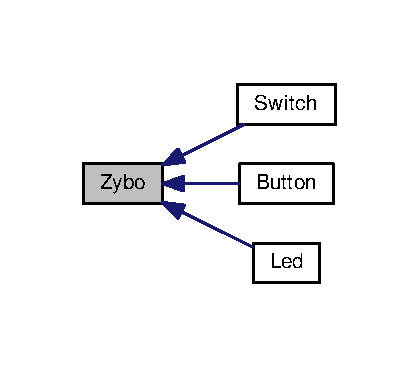
\includegraphics[width=201pt]{group___zybo}
\end{center}
\end{figure}
\subsection*{Moduli}
\begin{DoxyCompactItemize}
\item 
\hyperlink{group___button}{Button}
\item 
\hyperlink{group___led}{Led}
\item 
\hyperlink{group___switch}{Switch}
\end{DoxyCompactItemize}


\subsection{Descrizione dettagliata}

\chapter{Documentazione delle classi}
\hypertarget{struct_g_p_i_o__t}{\section{Riferimenti per la struct G\+P\+I\+O\+\_\+t}
\label{struct_g_p_i_o__t}\index{G\+P\+I\+O\+\_\+t@{G\+P\+I\+O\+\_\+t}}
}


Struttura che astrae un device G\+P\+I\+O.  




{\ttfamily \#include $<$gpio.\+h$>$}

\subsection*{Campi}
\begin{DoxyCompactItemize}
\item 
\hypertarget{struct_g_p_i_o__t_a79c591d5fa42efdf86abd98347fece90}{uint32\+\_\+t $\ast$ {\bfseries base\+\_\+address}}\label{struct_g_p_i_o__t_a79c591d5fa42efdf86abd98347fece90}

\item 
\hypertarget{struct_g_p_i_o__t_a09a2a45f731b02946ff6d3cd15c1a476}{uint8\+\_\+t {\bfseries width}}\label{struct_g_p_i_o__t_a09a2a45f731b02946ff6d3cd15c1a476}

\item 
\hypertarget{struct_g_p_i_o__t_a14886d03a6936e5edd25a9ad27af16bd}{uint8\+\_\+t {\bfseries enable\+\_\+offset}}\label{struct_g_p_i_o__t_a14886d03a6936e5edd25a9ad27af16bd}

\item 
\hypertarget{struct_g_p_i_o__t_abb65e5db6d4ad365a7c48d00e4af1f78}{uint8\+\_\+t {\bfseries write\+\_\+offset}}\label{struct_g_p_i_o__t_abb65e5db6d4ad365a7c48d00e4af1f78}

\item 
\hypertarget{struct_g_p_i_o__t_ab65acde67dc46f1d163e2ee468420b48}{uint8\+\_\+t {\bfseries read\+\_\+offset}}\label{struct_g_p_i_o__t_ab65acde67dc46f1d163e2ee468420b48}

\end{DoxyCompactItemize}


\subsection{Descrizione dettagliata}
Struttura che astrae un device G\+P\+I\+O. 

La documentazione per questa struct è stata generata a partire dal seguente file\+:\begin{DoxyCompactItemize}
\item 
G\+P\+I\+O/gpio.\+h\end{DoxyCompactItemize}

\hypertarget{struct_h_d44780___l_c_d__t}{\section{Riferimenti per la struct H\+D44780\+\_\+\+L\+C\+D\+\_\+t}
\label{struct_h_d44780___l_c_d__t}\index{H\+D44780\+\_\+\+L\+C\+D\+\_\+t@{H\+D44780\+\_\+\+L\+C\+D\+\_\+t}}
}


Struttura opaca che astrae un device Display L\+C\+D con cntroller Hitachi H\+D44780, o compatibile. Un oggetto di tipo \hyperlink{struct_h_d44780___l_c_d__t}{H\+D44780\+\_\+\+L\+C\+D\+\_\+t} rappresenta un device lcd H\+D44780. Il modulo e' pensato per permettere la gestione di piu' display da parte dello stesso processore, agendo su oggetti \hyperlink{struct_h_d44780___l_c_d__t}{H\+D44780\+\_\+\+L\+C\+D\+\_\+t} diversi. Il modulo permette di utilizzare sia l'interfacciamento ad otto bit che quello a quattro bit, inizializzando il device opportunamente, attraverso l'uso delle funzioni H\+D44780\+\_\+\+Init8 e\+H\+D44780\+\_\+\+Init4. Il modulo fornisce anche semplici funzioni per la stampa di un carattere o di una stringa null-\/terminated di caratteri. Si veda la documentazione delle funzioni H\+D44780\+\_\+\+Printc e H\+D44780\+\_\+\+Print. Inoltre sono presenti diverse funzioni di utilita' generica, come quelle per la pulizia del display, per lo spostamento del cursore di un posto in avanti o indietro, alla riga in basso o in alto.  




{\ttfamily \#include $<$hd44780.\+h$>$}

\subsection*{Campi}
\begin{DoxyCompactItemize}
\item 
G\+P\+I\+O\+\_\+t $\ast$ \hyperlink{struct_h_d44780___l_c_d__t_acb3116190992a4d8d26545c103304d27}{gpio}
\item 
G\+P\+I\+O\+\_\+mask \hyperlink{struct_h_d44780___l_c_d__t_a142ae0db638dca7ab42e2183a1311d32}{R\+S}
\item 
G\+P\+I\+O\+\_\+mask \hyperlink{struct_h_d44780___l_c_d__t_af8225e4a125a2159215dfa03372c305f}{R\+W}
\item 
G\+P\+I\+O\+\_\+mask \hyperlink{struct_h_d44780___l_c_d__t_a851ed1cefdadae2e5069d1364ae8fc9e}{E}
\item 
G\+P\+I\+O\+\_\+mask \hyperlink{struct_h_d44780___l_c_d__t_a7f1bd9ea66e1fa6d0667c3f60d2f155d}{Data7}
\item 
G\+P\+I\+O\+\_\+mask \hyperlink{struct_h_d44780___l_c_d__t_a6a787746d32e0e18dbd57202e547756b}{Data6}
\item 
G\+P\+I\+O\+\_\+mask \hyperlink{struct_h_d44780___l_c_d__t_aff5ae7b6e5cd6f96a13e719cd07e3f15}{Data5}
\item 
G\+P\+I\+O\+\_\+mask \hyperlink{struct_h_d44780___l_c_d__t_a923c685eba8920c56f33117410da2742}{Data4}
\item 
G\+P\+I\+O\+\_\+mask \hyperlink{struct_h_d44780___l_c_d__t_ae6f2e7b5a4aa8b82451e021f2f5b3a89}{Data3}
\item 
G\+P\+I\+O\+\_\+mask \hyperlink{struct_h_d44780___l_c_d__t_afb22274224118a94688f1809cda55501}{Data2}
\item 
G\+P\+I\+O\+\_\+mask \hyperlink{struct_h_d44780___l_c_d__t_a9b310a22b76c920feb015a3a3084b125}{Data1}
\item 
G\+P\+I\+O\+\_\+mask \hyperlink{struct_h_d44780___l_c_d__t_aed1ef3393be1a14aa7b2644585e5bb08}{Data0}
\item 
\hyperlink{group___h_d44780_gaaaea8b73e24f7658da4118f6b01b45f0}{H\+D44780\+\_\+\+Interface\+Mode\+\_\+t} \hyperlink{struct_h_d44780___l_c_d__t_a7c5a51b8cc5de5ee2cf42b884bd1bc67}{iface\+\_\+mode}
\end{DoxyCompactItemize}


\subsection{Descrizione dettagliata}
Struttura opaca che astrae un device Display L\+C\+D con cntroller Hitachi H\+D44780, o compatibile. Un oggetto di tipo \hyperlink{struct_h_d44780___l_c_d__t}{H\+D44780\+\_\+\+L\+C\+D\+\_\+t} rappresenta un device lcd H\+D44780. Il modulo e' pensato per permettere la gestione di piu' display da parte dello stesso processore, agendo su oggetti \hyperlink{struct_h_d44780___l_c_d__t}{H\+D44780\+\_\+\+L\+C\+D\+\_\+t} diversi. Il modulo permette di utilizzare sia l'interfacciamento ad otto bit che quello a quattro bit, inizializzando il device opportunamente, attraverso l'uso delle funzioni H\+D44780\+\_\+\+Init8 e\+H\+D44780\+\_\+\+Init4. Il modulo fornisce anche semplici funzioni per la stampa di un carattere o di una stringa null-\/terminated di caratteri. Si veda la documentazione delle funzioni H\+D44780\+\_\+\+Printc e H\+D44780\+\_\+\+Print. Inoltre sono presenti diverse funzioni di utilita' generica, come quelle per la pulizia del display, per lo spostamento del cursore di un posto in avanti o indietro, alla riga in basso o in alto. 

\subsection{Documentazione dei campi}
\hypertarget{struct_h_d44780___l_c_d__t_aed1ef3393be1a14aa7b2644585e5bb08}{\index{H\+D44780\+\_\+\+L\+C\+D\+\_\+t@{H\+D44780\+\_\+\+L\+C\+D\+\_\+t}!Data0@{Data0}}
\index{Data0@{Data0}!H\+D44780\+\_\+\+L\+C\+D\+\_\+t@{H\+D44780\+\_\+\+L\+C\+D\+\_\+t}}
\subsubsection[{Data0}]{\setlength{\rightskip}{0pt plus 5cm}G\+P\+I\+O\+\_\+mask Data0}}\label{struct_h_d44780___l_c_d__t_aed1ef3393be1a14aa7b2644585e5bb08}
maschera di selezione per il pin del device G\+P\+I\+O usato per il pilotaggio del segnale D0 \hypertarget{struct_h_d44780___l_c_d__t_a9b310a22b76c920feb015a3a3084b125}{\index{H\+D44780\+\_\+\+L\+C\+D\+\_\+t@{H\+D44780\+\_\+\+L\+C\+D\+\_\+t}!Data1@{Data1}}
\index{Data1@{Data1}!H\+D44780\+\_\+\+L\+C\+D\+\_\+t@{H\+D44780\+\_\+\+L\+C\+D\+\_\+t}}
\subsubsection[{Data1}]{\setlength{\rightskip}{0pt plus 5cm}G\+P\+I\+O\+\_\+mask Data1}}\label{struct_h_d44780___l_c_d__t_a9b310a22b76c920feb015a3a3084b125}
maschera di selezione per il pin del device G\+P\+I\+O usato per il pilotaggio del segnale D1 \hypertarget{struct_h_d44780___l_c_d__t_afb22274224118a94688f1809cda55501}{\index{H\+D44780\+\_\+\+L\+C\+D\+\_\+t@{H\+D44780\+\_\+\+L\+C\+D\+\_\+t}!Data2@{Data2}}
\index{Data2@{Data2}!H\+D44780\+\_\+\+L\+C\+D\+\_\+t@{H\+D44780\+\_\+\+L\+C\+D\+\_\+t}}
\subsubsection[{Data2}]{\setlength{\rightskip}{0pt plus 5cm}G\+P\+I\+O\+\_\+mask Data2}}\label{struct_h_d44780___l_c_d__t_afb22274224118a94688f1809cda55501}
maschera di selezione per il pin del device G\+P\+I\+O usato per il pilotaggio del segnale D2 \hypertarget{struct_h_d44780___l_c_d__t_ae6f2e7b5a4aa8b82451e021f2f5b3a89}{\index{H\+D44780\+\_\+\+L\+C\+D\+\_\+t@{H\+D44780\+\_\+\+L\+C\+D\+\_\+t}!Data3@{Data3}}
\index{Data3@{Data3}!H\+D44780\+\_\+\+L\+C\+D\+\_\+t@{H\+D44780\+\_\+\+L\+C\+D\+\_\+t}}
\subsubsection[{Data3}]{\setlength{\rightskip}{0pt plus 5cm}G\+P\+I\+O\+\_\+mask Data3}}\label{struct_h_d44780___l_c_d__t_ae6f2e7b5a4aa8b82451e021f2f5b3a89}
maschera di selezione per il pin del device G\+P\+I\+O usato per il pilotaggio del segnale D3 \hypertarget{struct_h_d44780___l_c_d__t_a923c685eba8920c56f33117410da2742}{\index{H\+D44780\+\_\+\+L\+C\+D\+\_\+t@{H\+D44780\+\_\+\+L\+C\+D\+\_\+t}!Data4@{Data4}}
\index{Data4@{Data4}!H\+D44780\+\_\+\+L\+C\+D\+\_\+t@{H\+D44780\+\_\+\+L\+C\+D\+\_\+t}}
\subsubsection[{Data4}]{\setlength{\rightskip}{0pt plus 5cm}G\+P\+I\+O\+\_\+mask Data4}}\label{struct_h_d44780___l_c_d__t_a923c685eba8920c56f33117410da2742}
maschera di selezione per il pin del device G\+P\+I\+O usato per il pilotaggio del segnale D4 \hypertarget{struct_h_d44780___l_c_d__t_aff5ae7b6e5cd6f96a13e719cd07e3f15}{\index{H\+D44780\+\_\+\+L\+C\+D\+\_\+t@{H\+D44780\+\_\+\+L\+C\+D\+\_\+t}!Data5@{Data5}}
\index{Data5@{Data5}!H\+D44780\+\_\+\+L\+C\+D\+\_\+t@{H\+D44780\+\_\+\+L\+C\+D\+\_\+t}}
\subsubsection[{Data5}]{\setlength{\rightskip}{0pt plus 5cm}G\+P\+I\+O\+\_\+mask Data5}}\label{struct_h_d44780___l_c_d__t_aff5ae7b6e5cd6f96a13e719cd07e3f15}
maschera di selezione per il pin del device G\+P\+I\+O usato per il pilotaggio del segnale D5 \hypertarget{struct_h_d44780___l_c_d__t_a6a787746d32e0e18dbd57202e547756b}{\index{H\+D44780\+\_\+\+L\+C\+D\+\_\+t@{H\+D44780\+\_\+\+L\+C\+D\+\_\+t}!Data6@{Data6}}
\index{Data6@{Data6}!H\+D44780\+\_\+\+L\+C\+D\+\_\+t@{H\+D44780\+\_\+\+L\+C\+D\+\_\+t}}
\subsubsection[{Data6}]{\setlength{\rightskip}{0pt plus 5cm}G\+P\+I\+O\+\_\+mask Data6}}\label{struct_h_d44780___l_c_d__t_a6a787746d32e0e18dbd57202e547756b}
maschera di selezione per il pin del device G\+P\+I\+O usato per il pilotaggio del segnale D6 \hypertarget{struct_h_d44780___l_c_d__t_a7f1bd9ea66e1fa6d0667c3f60d2f155d}{\index{H\+D44780\+\_\+\+L\+C\+D\+\_\+t@{H\+D44780\+\_\+\+L\+C\+D\+\_\+t}!Data7@{Data7}}
\index{Data7@{Data7}!H\+D44780\+\_\+\+L\+C\+D\+\_\+t@{H\+D44780\+\_\+\+L\+C\+D\+\_\+t}}
\subsubsection[{Data7}]{\setlength{\rightskip}{0pt plus 5cm}G\+P\+I\+O\+\_\+mask Data7}}\label{struct_h_d44780___l_c_d__t_a7f1bd9ea66e1fa6d0667c3f60d2f155d}
maschera di selezione per il pin del device G\+P\+I\+O usato per il pilotaggio del segnale D7 \hypertarget{struct_h_d44780___l_c_d__t_a851ed1cefdadae2e5069d1364ae8fc9e}{\index{H\+D44780\+\_\+\+L\+C\+D\+\_\+t@{H\+D44780\+\_\+\+L\+C\+D\+\_\+t}!E@{E}}
\index{E@{E}!H\+D44780\+\_\+\+L\+C\+D\+\_\+t@{H\+D44780\+\_\+\+L\+C\+D\+\_\+t}}
\subsubsection[{E}]{\setlength{\rightskip}{0pt plus 5cm}G\+P\+I\+O\+\_\+mask E}}\label{struct_h_d44780___l_c_d__t_a851ed1cefdadae2e5069d1364ae8fc9e}
maschera di selezione per il pin del device G\+P\+I\+O usato per il pilotaggio del segnale E \hypertarget{struct_h_d44780___l_c_d__t_acb3116190992a4d8d26545c103304d27}{\index{H\+D44780\+\_\+\+L\+C\+D\+\_\+t@{H\+D44780\+\_\+\+L\+C\+D\+\_\+t}!gpio@{gpio}}
\index{gpio@{gpio}!H\+D44780\+\_\+\+L\+C\+D\+\_\+t@{H\+D44780\+\_\+\+L\+C\+D\+\_\+t}}
\subsubsection[{gpio}]{\setlength{\rightskip}{0pt plus 5cm}G\+P\+I\+O\+\_\+t$\ast$ gpio}}\label{struct_h_d44780___l_c_d__t_acb3116190992a4d8d26545c103304d27}
puntatore a struttura G\+P\+I\+O\+\_\+t, che astrae il particolare G\+P\+I\+O usato per il pilotaggio del display \hypertarget{struct_h_d44780___l_c_d__t_a7c5a51b8cc5de5ee2cf42b884bd1bc67}{\index{H\+D44780\+\_\+\+L\+C\+D\+\_\+t@{H\+D44780\+\_\+\+L\+C\+D\+\_\+t}!iface\+\_\+mode@{iface\+\_\+mode}}
\index{iface\+\_\+mode@{iface\+\_\+mode}!H\+D44780\+\_\+\+L\+C\+D\+\_\+t@{H\+D44780\+\_\+\+L\+C\+D\+\_\+t}}
\subsubsection[{iface\+\_\+mode}]{\setlength{\rightskip}{0pt plus 5cm}{\bf H\+D44780\+\_\+\+Interface\+Mode\+\_\+t} iface\+\_\+mode}}\label{struct_h_d44780___l_c_d__t_a7c5a51b8cc5de5ee2cf42b884bd1bc67}
modalita' di funzionamento dell'interfaccia verso il displau (4 oppure 8 bit) \hypertarget{struct_h_d44780___l_c_d__t_a142ae0db638dca7ab42e2183a1311d32}{\index{H\+D44780\+\_\+\+L\+C\+D\+\_\+t@{H\+D44780\+\_\+\+L\+C\+D\+\_\+t}!R\+S@{R\+S}}
\index{R\+S@{R\+S}!H\+D44780\+\_\+\+L\+C\+D\+\_\+t@{H\+D44780\+\_\+\+L\+C\+D\+\_\+t}}
\subsubsection[{R\+S}]{\setlength{\rightskip}{0pt plus 5cm}G\+P\+I\+O\+\_\+mask R\+S}}\label{struct_h_d44780___l_c_d__t_a142ae0db638dca7ab42e2183a1311d32}
maschera di selezione per il pin del device G\+P\+I\+O usato per il pilotaggio del segnale R\+S \hypertarget{struct_h_d44780___l_c_d__t_af8225e4a125a2159215dfa03372c305f}{\index{H\+D44780\+\_\+\+L\+C\+D\+\_\+t@{H\+D44780\+\_\+\+L\+C\+D\+\_\+t}!R\+W@{R\+W}}
\index{R\+W@{R\+W}!H\+D44780\+\_\+\+L\+C\+D\+\_\+t@{H\+D44780\+\_\+\+L\+C\+D\+\_\+t}}
\subsubsection[{R\+W}]{\setlength{\rightskip}{0pt plus 5cm}G\+P\+I\+O\+\_\+mask R\+W}}\label{struct_h_d44780___l_c_d__t_af8225e4a125a2159215dfa03372c305f}
maschera di selezione per il pin del device G\+P\+I\+O usato per il pilotaggio del segnale R\+W 

La documentazione per questa struct è stata generata a partire dal seguente file\+:\begin{DoxyCompactItemize}
\item 
Lcd/\hyperlink{hd44780_8h}{hd44780.\+h}\end{DoxyCompactItemize}

\hypertarget{struct_zybo_button__t}{\section{Riferimenti per la struct Zybo\+Button\+\_\+t}
\label{struct_zybo_button__t}\index{Zybo\+Button\+\_\+t@{Zybo\+Button\+\_\+t}}
}


Struttura opaca che astrae l'insieme dei button presenti sulla board Digilent Zybo;.  




{\ttfamily \#include $<$Zybo\+Button.\+h$>$}



Diagramma di collaborazione per Zybo\+Button\+\_\+t\+:\nopagebreak
\begin{figure}[H]
\begin{center}
\leavevmode
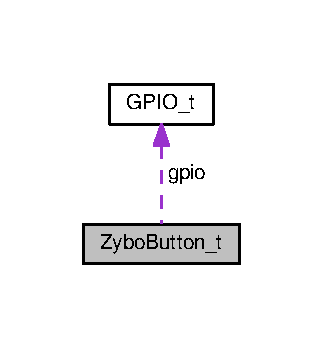
\includegraphics[width=155pt]{struct_zybo_button__t__coll__graph}
\end{center}
\end{figure}
\subsection*{Campi}
\begin{DoxyCompactItemize}
\item 
\hyperlink{structmy_g_p_i_o__t}{my\+G\+P\+I\+O\+\_\+t} $\ast$ \hyperlink{struct_zybo_button__t_ac37ddc7c58d246d233dfb38037020184}{gpio}
\item 
\hyperlink{group__bare-metal_ga402a0d20afc0cb7c25554b8b023f4253}{my\+G\+P\+I\+O\+\_\+mask} \hyperlink{struct_zybo_button__t_ad462a15a55883fd4c86d2be9e11968a7}{Button3\+\_\+pin}
\item 
\hyperlink{group__bare-metal_ga402a0d20afc0cb7c25554b8b023f4253}{my\+G\+P\+I\+O\+\_\+mask} \hyperlink{struct_zybo_button__t_a3b4fe634c2d98ce55fdef526c2d230d1}{Button2\+\_\+pin}
\item 
\hyperlink{group__bare-metal_ga402a0d20afc0cb7c25554b8b023f4253}{my\+G\+P\+I\+O\+\_\+mask} \hyperlink{struct_zybo_button__t_a6cb60bb285e32e29c51c15e85206aaeb}{Button1\+\_\+pin}
\item 
\hyperlink{group__bare-metal_ga402a0d20afc0cb7c25554b8b023f4253}{my\+G\+P\+I\+O\+\_\+mask} \hyperlink{struct_zybo_button__t_af7d7d5a9c9fc174e8f4ee4c762c2abee}{Button0\+\_\+pin}
\end{DoxyCompactItemize}


\subsection{Descrizione dettagliata}
Struttura opaca che astrae l'insieme dei button presenti sulla board Digilent Zybo;. \begin{Desc}
\item[Esempi\+: ]\par
\hyperlink{bsp_example_8c-example}{bsp\+\_\+example.\+c}.\end{Desc}


\subsection{Documentazione dei campi}
\hypertarget{struct_zybo_button__t_af7d7d5a9c9fc174e8f4ee4c762c2abee}{\index{Zybo\+Button\+\_\+t@{Zybo\+Button\+\_\+t}!Button0\+\_\+pin@{Button0\+\_\+pin}}
\index{Button0\+\_\+pin@{Button0\+\_\+pin}!Zybo\+Button\+\_\+t@{Zybo\+Button\+\_\+t}}
\subsubsection[{Button0\+\_\+pin}]{\setlength{\rightskip}{0pt plus 5cm}{\bf my\+G\+P\+I\+O\+\_\+mask} Button0\+\_\+pin}}\label{struct_zybo_button__t_af7d7d5a9c9fc174e8f4ee4c762c2abee}
maschera di selezione per il particolare bit del device my\+G\+P\+I\+O connesso al button numero 0 della board Zybo \hypertarget{struct_zybo_button__t_a6cb60bb285e32e29c51c15e85206aaeb}{\index{Zybo\+Button\+\_\+t@{Zybo\+Button\+\_\+t}!Button1\+\_\+pin@{Button1\+\_\+pin}}
\index{Button1\+\_\+pin@{Button1\+\_\+pin}!Zybo\+Button\+\_\+t@{Zybo\+Button\+\_\+t}}
\subsubsection[{Button1\+\_\+pin}]{\setlength{\rightskip}{0pt plus 5cm}{\bf my\+G\+P\+I\+O\+\_\+mask} Button1\+\_\+pin}}\label{struct_zybo_button__t_a6cb60bb285e32e29c51c15e85206aaeb}
maschera di selezione per il particolare bit del device my\+G\+P\+I\+O connesso al button numero 1 della board Zybo \hypertarget{struct_zybo_button__t_a3b4fe634c2d98ce55fdef526c2d230d1}{\index{Zybo\+Button\+\_\+t@{Zybo\+Button\+\_\+t}!Button2\+\_\+pin@{Button2\+\_\+pin}}
\index{Button2\+\_\+pin@{Button2\+\_\+pin}!Zybo\+Button\+\_\+t@{Zybo\+Button\+\_\+t}}
\subsubsection[{Button2\+\_\+pin}]{\setlength{\rightskip}{0pt plus 5cm}{\bf my\+G\+P\+I\+O\+\_\+mask} Button2\+\_\+pin}}\label{struct_zybo_button__t_a3b4fe634c2d98ce55fdef526c2d230d1}
maschera di selezione per il particolare bit del device my\+G\+P\+I\+O connesso al button numero 2 della board Zybo \hypertarget{struct_zybo_button__t_ad462a15a55883fd4c86d2be9e11968a7}{\index{Zybo\+Button\+\_\+t@{Zybo\+Button\+\_\+t}!Button3\+\_\+pin@{Button3\+\_\+pin}}
\index{Button3\+\_\+pin@{Button3\+\_\+pin}!Zybo\+Button\+\_\+t@{Zybo\+Button\+\_\+t}}
\subsubsection[{Button3\+\_\+pin}]{\setlength{\rightskip}{0pt plus 5cm}{\bf my\+G\+P\+I\+O\+\_\+mask} Button3\+\_\+pin}}\label{struct_zybo_button__t_ad462a15a55883fd4c86d2be9e11968a7}
maschera di selezione per il particolare bit del device my\+G\+P\+I\+O connesso al button numero 3 della board Zybo \hypertarget{struct_zybo_button__t_ac37ddc7c58d246d233dfb38037020184}{\index{Zybo\+Button\+\_\+t@{Zybo\+Button\+\_\+t}!gpio@{gpio}}
\index{gpio@{gpio}!Zybo\+Button\+\_\+t@{Zybo\+Button\+\_\+t}}
\subsubsection[{gpio}]{\setlength{\rightskip}{0pt plus 5cm}{\bf my\+G\+P\+I\+O\+\_\+t}$\ast$ gpio}}\label{struct_zybo_button__t_ac37ddc7c58d246d233dfb38037020184}
puntatore a struttura \hyperlink{structmy_g_p_i_o__t}{my\+G\+P\+I\+O\+\_\+t}, che astrae il particolare my\+G\+P\+I\+O usato per la lettura dello stato dei button presenti sulla board 

La documentazione per questa struct è stata generata a partire dal seguente file\+:\begin{DoxyCompactItemize}
\item 
Src/my\+G\+P\+I\+O/bare-\/metal/\+Zybo\+B\+S\+P/\hyperlink{_zybo_button_8h}{Zybo\+Button.\+h}\end{DoxyCompactItemize}

\hypertarget{struct_zybo_led__t}{\section{Riferimenti per la struct Zybo\+Led\+\_\+t}
\label{struct_zybo_led__t}\index{Zybo\+Led\+\_\+t@{Zybo\+Led\+\_\+t}}
}


Struttura opaca che astrae l'insieme dei Led presenti sulla board Digilent Zybo;.  




{\ttfamily \#include $<$Zybo\+Led.\+h$>$}



Diagramma di collaborazione per Zybo\+Led\+\_\+t\+:
\nopagebreak
\begin{figure}[H]
\begin{center}
\leavevmode
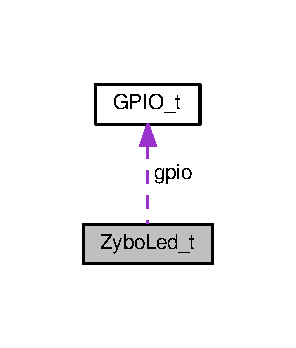
\includegraphics[width=143pt]{struct_zybo_led__t__coll__graph}
\end{center}
\end{figure}
\subsection*{Campi}
\begin{DoxyCompactItemize}
\item 
\hyperlink{structmy_g_p_i_o__t}{my\+G\+P\+I\+O\+\_\+t} $\ast$ \hyperlink{struct_zybo_led__t_ac37ddc7c58d246d233dfb38037020184}{gpio}
\item 
\hyperlink{group__my_g_p_i_o_ga402a0d20afc0cb7c25554b8b023f4253}{my\+G\+P\+I\+O\+\_\+mask} \hyperlink{struct_zybo_led__t_afc64d1407f30615e374bf9f06721842a}{Led3\+\_\+pin}
\item 
\hyperlink{group__my_g_p_i_o_ga402a0d20afc0cb7c25554b8b023f4253}{my\+G\+P\+I\+O\+\_\+mask} \hyperlink{struct_zybo_led__t_a4213c78e5a02b1476222e989c2eceb04}{Led2\+\_\+pin}
\item 
\hyperlink{group__my_g_p_i_o_ga402a0d20afc0cb7c25554b8b023f4253}{my\+G\+P\+I\+O\+\_\+mask} \hyperlink{struct_zybo_led__t_adc78fb167f1dd6693910813d4ec5930e}{Led1\+\_\+pin}
\item 
\hyperlink{group__my_g_p_i_o_ga402a0d20afc0cb7c25554b8b023f4253}{my\+G\+P\+I\+O\+\_\+mask} \hyperlink{struct_zybo_led__t_ac5afef2eef91d5533a23435cfcc60104}{Led0\+\_\+pin}
\end{DoxyCompactItemize}


\subsection{Descrizione dettagliata}
Struttura opaca che astrae l'insieme dei Led presenti sulla board Digilent Zybo;. 

\subsection{Documentazione dei campi}
\hypertarget{struct_zybo_led__t_ac37ddc7c58d246d233dfb38037020184}{\index{Zybo\+Led\+\_\+t@{Zybo\+Led\+\_\+t}!gpio@{gpio}}
\index{gpio@{gpio}!Zybo\+Led\+\_\+t@{Zybo\+Led\+\_\+t}}
\subsubsection[{gpio}]{\setlength{\rightskip}{0pt plus 5cm}{\bf my\+G\+P\+I\+O\+\_\+t}$\ast$ gpio}}\label{struct_zybo_led__t_ac37ddc7c58d246d233dfb38037020184}
puntatore a struttura \hyperlink{structmy_g_p_i_o__t}{my\+G\+P\+I\+O\+\_\+t}, che astrae il particolare G\+P\+I\+O usato per il pilotaggio dei led presenti sulla board \hypertarget{struct_zybo_led__t_ac5afef2eef91d5533a23435cfcc60104}{\index{Zybo\+Led\+\_\+t@{Zybo\+Led\+\_\+t}!Led0\+\_\+pin@{Led0\+\_\+pin}}
\index{Led0\+\_\+pin@{Led0\+\_\+pin}!Zybo\+Led\+\_\+t@{Zybo\+Led\+\_\+t}}
\subsubsection[{Led0\+\_\+pin}]{\setlength{\rightskip}{0pt plus 5cm}{\bf my\+G\+P\+I\+O\+\_\+mask} Led0\+\_\+pin}}\label{struct_zybo_led__t_ac5afef2eef91d5533a23435cfcc60104}
maschera di selezione per il particolare bit del device G\+P\+I\+O usato per il pilotaggio del led numero 0 della board Zybo \hypertarget{struct_zybo_led__t_adc78fb167f1dd6693910813d4ec5930e}{\index{Zybo\+Led\+\_\+t@{Zybo\+Led\+\_\+t}!Led1\+\_\+pin@{Led1\+\_\+pin}}
\index{Led1\+\_\+pin@{Led1\+\_\+pin}!Zybo\+Led\+\_\+t@{Zybo\+Led\+\_\+t}}
\subsubsection[{Led1\+\_\+pin}]{\setlength{\rightskip}{0pt plus 5cm}{\bf my\+G\+P\+I\+O\+\_\+mask} Led1\+\_\+pin}}\label{struct_zybo_led__t_adc78fb167f1dd6693910813d4ec5930e}
maschera di selezione per il particolare bit del device G\+P\+I\+O usato per il pilotaggio del led numero 1 della board Zybo \hypertarget{struct_zybo_led__t_a4213c78e5a02b1476222e989c2eceb04}{\index{Zybo\+Led\+\_\+t@{Zybo\+Led\+\_\+t}!Led2\+\_\+pin@{Led2\+\_\+pin}}
\index{Led2\+\_\+pin@{Led2\+\_\+pin}!Zybo\+Led\+\_\+t@{Zybo\+Led\+\_\+t}}
\subsubsection[{Led2\+\_\+pin}]{\setlength{\rightskip}{0pt plus 5cm}{\bf my\+G\+P\+I\+O\+\_\+mask} Led2\+\_\+pin}}\label{struct_zybo_led__t_a4213c78e5a02b1476222e989c2eceb04}
maschera di selezione per il particolare bit del device G\+P\+I\+O usato per il pilotaggio del led numero 2 della board Zybo \hypertarget{struct_zybo_led__t_afc64d1407f30615e374bf9f06721842a}{\index{Zybo\+Led\+\_\+t@{Zybo\+Led\+\_\+t}!Led3\+\_\+pin@{Led3\+\_\+pin}}
\index{Led3\+\_\+pin@{Led3\+\_\+pin}!Zybo\+Led\+\_\+t@{Zybo\+Led\+\_\+t}}
\subsubsection[{Led3\+\_\+pin}]{\setlength{\rightskip}{0pt plus 5cm}{\bf my\+G\+P\+I\+O\+\_\+mask} Led3\+\_\+pin}}\label{struct_zybo_led__t_afc64d1407f30615e374bf9f06721842a}
maschera di selezione per il particolare bit del device G\+P\+I\+O usato per il pilotaggio del led numero 3 della board Zybo 

La documentazione per questa struct è stata generata a partire dal seguente file\+:\begin{DoxyCompactItemize}
\item 
Zybo/\hyperlink{_zybo_led_8h}{Zybo\+Led.\+h}\end{DoxyCompactItemize}

\hypertarget{struct_zybo_switch__t}{\section{Riferimenti per la struct Zybo\+Switch\+\_\+t}
\label{struct_zybo_switch__t}\index{Zybo\+Switch\+\_\+t@{Zybo\+Switch\+\_\+t}}
}


Struttura opaca che astrae l'insieme degli switch presenti sulla board Digilent Zybo;.  




{\ttfamily \#include $<$Zybo\+Switch.\+h$>$}



Diagramma di collaborazione per Zybo\+Switch\+\_\+t\+:
\nopagebreak
\begin{figure}[H]
\begin{center}
\leavevmode
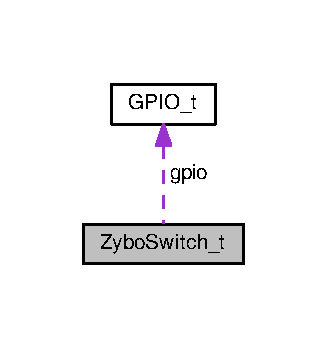
\includegraphics[width=157pt]{struct_zybo_switch__t__coll__graph}
\end{center}
\end{figure}
\subsection*{Campi}
\begin{DoxyCompactItemize}
\item 
\hypertarget{struct_zybo_switch__t_acb3116190992a4d8d26545c103304d27}{\hyperlink{struct_g_p_i_o__t}{G\+P\+I\+O\+\_\+t} $\ast$ {\bfseries gpio}}\label{struct_zybo_switch__t_acb3116190992a4d8d26545c103304d27}

\item 
\hypertarget{struct_zybo_switch__t_a6b95420b88fe8c1fd7f347ce3ae1906b}{G\+P\+I\+O\+\_\+mask {\bfseries Switch3\+\_\+pin}}\label{struct_zybo_switch__t_a6b95420b88fe8c1fd7f347ce3ae1906b}

\item 
\hypertarget{struct_zybo_switch__t_a33eda4a0115ef585edd90078924ca56e}{G\+P\+I\+O\+\_\+mask {\bfseries Switch2\+\_\+pin}}\label{struct_zybo_switch__t_a33eda4a0115ef585edd90078924ca56e}

\item 
\hypertarget{struct_zybo_switch__t_a6a3a5739e7e8f138241cafeeb7c1a33f}{G\+P\+I\+O\+\_\+mask {\bfseries Switch1\+\_\+pin}}\label{struct_zybo_switch__t_a6a3a5739e7e8f138241cafeeb7c1a33f}

\item 
\hypertarget{struct_zybo_switch__t_a5b7f83cd96441b7d1692710c6499147c}{G\+P\+I\+O\+\_\+mask {\bfseries Switch0\+\_\+pin}}\label{struct_zybo_switch__t_a5b7f83cd96441b7d1692710c6499147c}

\end{DoxyCompactItemize}


\subsection{Descrizione dettagliata}
Struttura opaca che astrae l'insieme degli switch presenti sulla board Digilent Zybo;. 

La documentazione per questa struct è stata generata a partire dal seguente file\+:\begin{DoxyCompactItemize}
\item 
Zybo/Zybo\+Switch.\+h\end{DoxyCompactItemize}

\chapter{Documentazione dei file}
\hypertarget{gpio_8c}{\section{Riferimenti per il file G\+P\+I\+O/gpio.c}
\label{gpio_8c}\index{G\+P\+I\+O/gpio.\+c@{G\+P\+I\+O/gpio.\+c}}
}
{\ttfamily \#include \char`\"{}gpio.\+h\char`\"{}}\\*
{\ttfamily \#include $<$stdlib.\+h$>$}\\*
{\ttfamily \#include $<$assert.\+h$>$}\\*
Grafo delle dipendenze di inclusione per gpio.\+c\+:\nopagebreak
\begin{figure}[H]
\begin{center}
\leavevmode
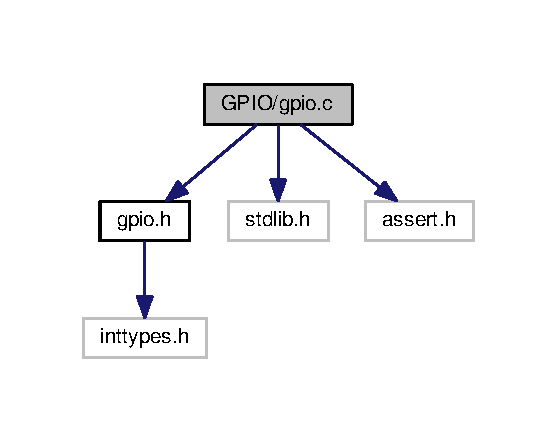
\includegraphics[width=268pt]{gpio_8c__incl}
\end{center}
\end{figure}
\subsection*{Funzioni}
\begin{DoxyCompactItemize}
\item 
void \hyperlink{group___g_p_i_o_gad3d8f07163fbe858774e769eb6d755db}{G\+P\+I\+O\+\_\+init} (\hyperlink{struct_g_p_i_o__t}{G\+P\+I\+O\+\_\+t} $\ast$gpio, uint32\+\_\+t $\ast$base\+\_\+address, uint8\+\_\+t width, uint8\+\_\+t enable\+\_\+offset, uint8\+\_\+t write\+\_\+offset, uint8\+\_\+t read\+\_\+offset)
\begin{DoxyCompactList}\small\item\em Inizializza un device G\+P\+I\+O. \end{DoxyCompactList}\item 
void \hyperlink{group___g_p_i_o_ga3f18ccfbb70d89cc7e2b06712dd82eb7}{G\+P\+I\+O\+\_\+set\+Mode} (\hyperlink{struct_g_p_i_o__t}{G\+P\+I\+O\+\_\+t} $\ast$gpio, \hyperlink{group___g_p_i_o_ga6d5aef8a8a54ee2f602d47252ff66595}{G\+P\+I\+O\+\_\+mask} mask, \hyperlink{group___g_p_i_o_ga894e6ae857ed4a9aedd04fff44a6770e}{G\+P\+I\+O\+\_\+mode} mode)
\begin{DoxyCompactList}\small\item\em Permette di settare la modalita' lettura/scrittura dei pin di un device G\+P\+I\+O;. \end{DoxyCompactList}\item 
void \hyperlink{group___g_p_i_o_ga86b232ed74eacf9aa723cb1d7917a156}{G\+P\+I\+O\+\_\+set\+Value} (\hyperlink{struct_g_p_i_o__t}{G\+P\+I\+O\+\_\+t} $\ast$gpio, \hyperlink{group___g_p_i_o_ga6d5aef8a8a54ee2f602d47252ff66595}{G\+P\+I\+O\+\_\+mask} mask, \hyperlink{group___g_p_i_o_ga495d9a7aa735fe416a3f110337c54967}{G\+P\+I\+O\+\_\+value} value)
\begin{DoxyCompactList}\small\item\em Permette di settare il valore dei pin di un device G\+P\+I\+O;. \end{DoxyCompactList}\item 
void \hyperlink{group___g_p_i_o_ga2f516854e98cd048d4d1ee6f86261f8c}{G\+P\+I\+O\+\_\+toggle} (\hyperlink{struct_g_p_i_o__t}{G\+P\+I\+O\+\_\+t} $\ast$gpio, \hyperlink{group___g_p_i_o_ga6d5aef8a8a54ee2f602d47252ff66595}{G\+P\+I\+O\+\_\+mask} mask)
\begin{DoxyCompactList}\small\item\em Permette di invertire il valore dei pin di un device G\+P\+I\+O;. \end{DoxyCompactList}\item 
\hyperlink{group___g_p_i_o_ga495d9a7aa735fe416a3f110337c54967}{G\+P\+I\+O\+\_\+value} \hyperlink{group___g_p_i_o_gaf388b01cd7459baae5c03c744f611724}{G\+P\+I\+O\+\_\+get\+Value} (\hyperlink{struct_g_p_i_o__t}{G\+P\+I\+O\+\_\+t} $\ast$gpio, \hyperlink{group___g_p_i_o_ga6d5aef8a8a54ee2f602d47252ff66595}{G\+P\+I\+O\+\_\+mask} mask)
\begin{DoxyCompactList}\small\item\em Permette di leggere il valore dei pin di un device G\+P\+I\+O;. \end{DoxyCompactList}\end{DoxyCompactItemize}

\hypertarget{gpio_8h}{\section{Riferimenti per il file G\+P\+I\+O/gpio.h}
\label{gpio_8h}\index{G\+P\+I\+O/gpio.\+h@{G\+P\+I\+O/gpio.\+h}}
}
{\ttfamily \#include $<$inttypes.\+h$>$}\\*
Grafo delle dipendenze di inclusione per gpio.\+h\+:\nopagebreak
\begin{figure}[H]
\begin{center}
\leavevmode
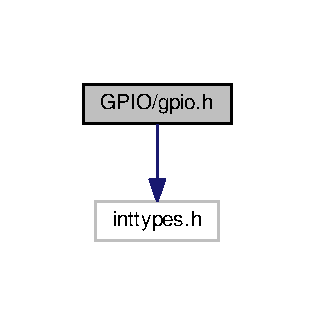
\includegraphics[width=151pt]{gpio_8h__incl}
\end{center}
\end{figure}
Questo grafo mostra quali altri file includono direttamente o indirettamente questo file\+:
\nopagebreak
\begin{figure}[H]
\begin{center}
\leavevmode
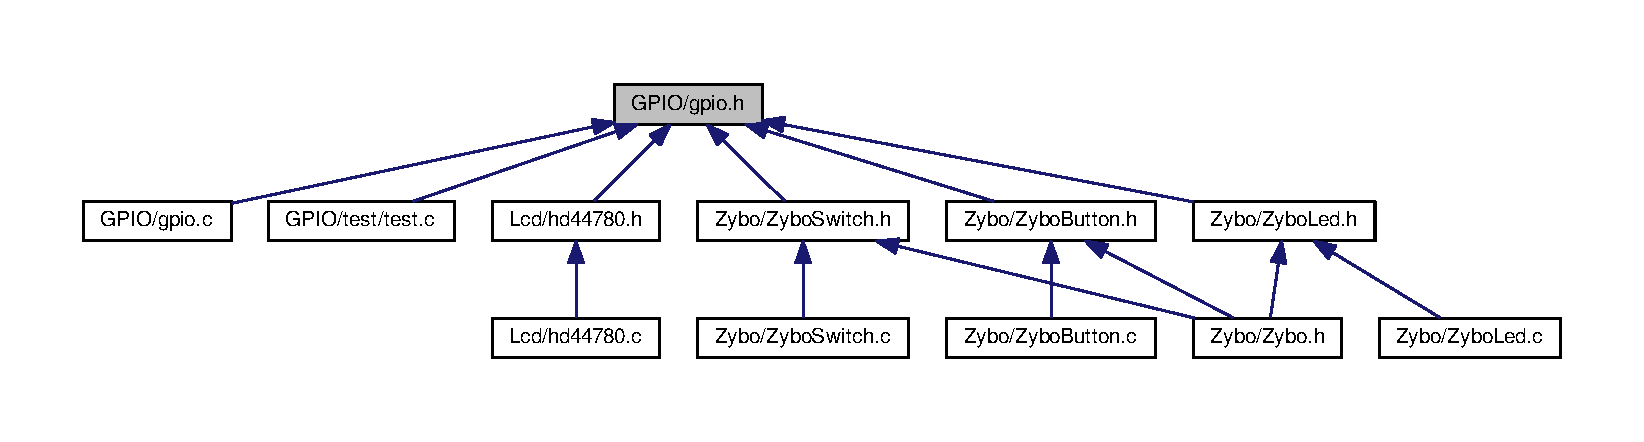
\includegraphics[width=350pt]{gpio_8h__dep__incl}
\end{center}
\end{figure}
\subsection*{Strutture dati}
\begin{DoxyCompactItemize}
\item 
struct \hyperlink{struct_g_p_i_o__t}{G\+P\+I\+O\+\_\+t}
\begin{DoxyCompactList}\small\item\em Struttura che astrae un device G\+P\+I\+O. \end{DoxyCompactList}\end{DoxyCompactItemize}
\subsection*{Definizioni}
\begin{DoxyCompactItemize}
\item 
\#define \hyperlink{group___g_p_i_o_ga8ac4b8e7e6313a8b139ef0e9f9781a0b}{G\+P\+I\+O\+\_\+pin}(i)~((uint32\+\_\+t)(1$<$$<$i))
\begin{DoxyCompactList}\small\item\em Metodo alternativo per la specifica di uno dei pin di un device G\+P\+I\+O. \end{DoxyCompactList}\end{DoxyCompactItemize}
\subsection*{Tipi enumerati (enum)}
\begin{DoxyCompactItemize}
\item 
enum \hyperlink{group___g_p_i_o_ga6d5aef8a8a54ee2f602d47252ff66595}{G\+P\+I\+O\+\_\+mask} \{ \\*
\hyperlink{group___g_p_i_o_gga6d5aef8a8a54ee2f602d47252ff66595adcbdf41a3086c14917c16aa16fe8dce0}{G\+P\+I\+O\+\_\+pin0} = 0x1, 
\hyperlink{group___g_p_i_o_gga6d5aef8a8a54ee2f602d47252ff66595a47f866a19d9ff54b424a644e879ab137}{G\+P\+I\+O\+\_\+pin1} = 0x2, 
\hyperlink{group___g_p_i_o_gga6d5aef8a8a54ee2f602d47252ff66595af020e3ce7822bbfad6c6c259bba650f8}{G\+P\+I\+O\+\_\+pin2} = 0x4, 
\hyperlink{group___g_p_i_o_gga6d5aef8a8a54ee2f602d47252ff66595ab5034fbdfc700bfe777088325fa2a448}{G\+P\+I\+O\+\_\+pin3} = 0x8, 
\\*
\hyperlink{group___g_p_i_o_gga6d5aef8a8a54ee2f602d47252ff66595a178596b752aa47edc06017af21862b10}{G\+P\+I\+O\+\_\+pin4} = 0x10, 
\hyperlink{group___g_p_i_o_gga6d5aef8a8a54ee2f602d47252ff66595aea86e18245853475d93732bda835a658}{G\+P\+I\+O\+\_\+pin5} = 0x20, 
\hyperlink{group___g_p_i_o_gga6d5aef8a8a54ee2f602d47252ff66595a29e82f4b193ce85e5d36546030dd8cdb}{G\+P\+I\+O\+\_\+pin6} = 0x40, 
\hyperlink{group___g_p_i_o_gga6d5aef8a8a54ee2f602d47252ff66595a593a4b6c0c46ac236fb50fbbba6eaa94}{G\+P\+I\+O\+\_\+pin7} = 0x80, 
\\*
\hyperlink{group___g_p_i_o_gga6d5aef8a8a54ee2f602d47252ff66595a25b17f4e7b1cbf2c8cd09f7049bf8e3c}{G\+P\+I\+O\+\_\+pin8} = 0x100, 
\hyperlink{group___g_p_i_o_gga6d5aef8a8a54ee2f602d47252ff66595a6b95a92fcb5f5a07947ee0eb0f0b9745}{G\+P\+I\+O\+\_\+pin9} = 0x200, 
\hyperlink{group___g_p_i_o_gga6d5aef8a8a54ee2f602d47252ff66595ac16a97d0cb0ab4064462b8e90f431444}{G\+P\+I\+O\+\_\+pin10} = 0x400, 
\hyperlink{group___g_p_i_o_gga6d5aef8a8a54ee2f602d47252ff66595a30f4930e20283fc8bb8897c21bbef6fe}{G\+P\+I\+O\+\_\+pin11} = 0x800, 
\\*
\hyperlink{group___g_p_i_o_gga6d5aef8a8a54ee2f602d47252ff66595af38edbc7a6b5ad7707b45f633879b5a6}{G\+P\+I\+O\+\_\+pin12} = 0x1000, 
\hyperlink{group___g_p_i_o_gga6d5aef8a8a54ee2f602d47252ff66595a7238a678f95a665e82c974cd6e64063b}{G\+P\+I\+O\+\_\+pin13} = 0x2000, 
\hyperlink{group___g_p_i_o_gga6d5aef8a8a54ee2f602d47252ff66595a6d0450f7184d9e30f292609fdb702021}{G\+P\+I\+O\+\_\+pin14} = 0x4000, 
\hyperlink{group___g_p_i_o_gga6d5aef8a8a54ee2f602d47252ff66595a2331cdf16345b682aa5a4aae88b7bfd7}{G\+P\+I\+O\+\_\+pin15} = 0x8000, 
\\*
\hyperlink{group___g_p_i_o_gga6d5aef8a8a54ee2f602d47252ff66595a47e8e2e95a483b8804336ebe8006bbdd}{G\+P\+I\+O\+\_\+pin16} = 0x10000, 
\hyperlink{group___g_p_i_o_gga6d5aef8a8a54ee2f602d47252ff66595afd25054cc3f6057842f12e9b461e04c5}{G\+P\+I\+O\+\_\+pin17} = 0x20000, 
\hyperlink{group___g_p_i_o_gga6d5aef8a8a54ee2f602d47252ff66595a0695e489ab495b018a134b1f3d654b03}{G\+P\+I\+O\+\_\+pin18} = 0x40000, 
\hyperlink{group___g_p_i_o_gga6d5aef8a8a54ee2f602d47252ff66595a951a5bd12a5ce5079380b66814bc7d4b}{G\+P\+I\+O\+\_\+pin19} = 0x80000, 
\\*
\hyperlink{group___g_p_i_o_gga6d5aef8a8a54ee2f602d47252ff66595a4cac847517ef83df4ec954d0d1937a21}{G\+P\+I\+O\+\_\+pin20} = 0x100000, 
\hyperlink{group___g_p_i_o_gga6d5aef8a8a54ee2f602d47252ff66595ab53658c53d924fd4310b948e6f2ac9a6}{G\+P\+I\+O\+\_\+pin21} = 0x200000, 
\hyperlink{group___g_p_i_o_gga6d5aef8a8a54ee2f602d47252ff66595ad72f6d42b4b0af56c73db6e50765f899}{G\+P\+I\+O\+\_\+pin22} = 0x400000, 
\hyperlink{group___g_p_i_o_gga6d5aef8a8a54ee2f602d47252ff66595a325ca3d5d92005391a0b125ead02af7b}{G\+P\+I\+O\+\_\+pin23} = 0x800000, 
\\*
\hyperlink{group___g_p_i_o_gga6d5aef8a8a54ee2f602d47252ff66595a4b85e0412ff080dfe5f10aeb981dad8f}{G\+P\+I\+O\+\_\+pin24} = 0x1000000, 
\hyperlink{group___g_p_i_o_gga6d5aef8a8a54ee2f602d47252ff66595ac5221e21fc0c958892c6238838b637ed}{G\+P\+I\+O\+\_\+pin25} = 0x2000000, 
\hyperlink{group___g_p_i_o_gga6d5aef8a8a54ee2f602d47252ff66595a6945a183851232023f40f47222c3dc77}{G\+P\+I\+O\+\_\+pin26} = 0x4000000, 
\hyperlink{group___g_p_i_o_gga6d5aef8a8a54ee2f602d47252ff66595a39d4771a24a35c485af5db41e458dfd5}{G\+P\+I\+O\+\_\+pin27} = 0x8000000, 
\\*
\hyperlink{group___g_p_i_o_gga6d5aef8a8a54ee2f602d47252ff66595a3ed32d8f1442759cabff7abda8dd9cdb}{G\+P\+I\+O\+\_\+pin28} = 0x10000000, 
\hyperlink{group___g_p_i_o_gga6d5aef8a8a54ee2f602d47252ff66595a751529bf657ad303e5e5c67a703138fe}{G\+P\+I\+O\+\_\+pin29} = 0x20000000, 
\hyperlink{group___g_p_i_o_gga6d5aef8a8a54ee2f602d47252ff66595a50add0846388b745f32ac8834f93de70}{G\+P\+I\+O\+\_\+pin30} = 0x40000000, 
\hyperlink{group___g_p_i_o_gga6d5aef8a8a54ee2f602d47252ff66595ab9d0bda88540c4e7ad5610009cd64d70}{G\+P\+I\+O\+\_\+pin31} = 0x80000000, 
\\*
\hyperlink{group___g_p_i_o_gga6d5aef8a8a54ee2f602d47252ff66595a8f89521ea70b3aed4a18c33a099b98d0}{G\+P\+I\+O\+\_\+byte0} = 0x000000ff, 
\hyperlink{group___g_p_i_o_gga6d5aef8a8a54ee2f602d47252ff66595a2a36eaac21d68a35dd3b3d1f790b4431}{G\+P\+I\+O\+\_\+byte1} = 0x0000ff00, 
\hyperlink{group___g_p_i_o_gga6d5aef8a8a54ee2f602d47252ff66595acf385bd78e3d36725f9d82955fce5fcf}{G\+P\+I\+O\+\_\+byte2} = 0x00ff0000, 
\hyperlink{group___g_p_i_o_gga6d5aef8a8a54ee2f602d47252ff66595adf78991a114e960df39d947c450de88c}{G\+P\+I\+O\+\_\+byte3} = 0xff000000
 \}
\begin{DoxyCompactList}\small\item\em Maschere di selezione dei pin di un device G\+P\+I\+O. \end{DoxyCompactList}\item 
enum \hyperlink{group___g_p_i_o_ga894e6ae857ed4a9aedd04fff44a6770e}{G\+P\+I\+O\+\_\+mode} \{ \hyperlink{group___g_p_i_o_gga894e6ae857ed4a9aedd04fff44a6770ea3db3c7d228d9b87cc125c8974241c800}{G\+P\+I\+O\+\_\+read}, 
\hyperlink{group___g_p_i_o_gga894e6ae857ed4a9aedd04fff44a6770eab1b932c1d800b09eb45b7ff5750bf73c}{G\+P\+I\+O\+\_\+write}
 \}
\begin{DoxyCompactList}\small\item\em G\+P\+I\+O\+\_\+mode, modalita' di funzionamento (lettura/scrittura) di un device G\+P\+I\+O. \end{DoxyCompactList}\item 
enum \hyperlink{group___g_p_i_o_ga495d9a7aa735fe416a3f110337c54967}{G\+P\+I\+O\+\_\+value} \{ \hyperlink{group___g_p_i_o_gga495d9a7aa735fe416a3f110337c54967a93cbe0e318453de590a9cb0030a840fa}{G\+P\+I\+O\+\_\+reset}, 
\hyperlink{group___g_p_i_o_gga495d9a7aa735fe416a3f110337c54967a39769e54aa8c4b6fbad0ef4ae88b5c44}{G\+P\+I\+O\+\_\+set}
 \}
\begin{DoxyCompactList}\small\item\em G\+P\+I\+O\+\_\+value. \end{DoxyCompactList}\end{DoxyCompactItemize}
\subsection*{Funzioni}
\begin{DoxyCompactItemize}
\item 
void \hyperlink{group___g_p_i_o_gad3d8f07163fbe858774e769eb6d755db}{G\+P\+I\+O\+\_\+init} (\hyperlink{struct_g_p_i_o__t}{G\+P\+I\+O\+\_\+t} $\ast$gpio, uint32\+\_\+t $\ast$base\+\_\+address, uint8\+\_\+t width, uint8\+\_\+t enable\+\_\+offset, uint8\+\_\+t write\+\_\+offset, uint8\+\_\+t read\+\_\+offset)
\begin{DoxyCompactList}\small\item\em Inizializza un device G\+P\+I\+O. \end{DoxyCompactList}\item 
void \hyperlink{group___g_p_i_o_ga3f18ccfbb70d89cc7e2b06712dd82eb7}{G\+P\+I\+O\+\_\+set\+Mode} (\hyperlink{struct_g_p_i_o__t}{G\+P\+I\+O\+\_\+t} $\ast$gpio, \hyperlink{group___g_p_i_o_ga6d5aef8a8a54ee2f602d47252ff66595}{G\+P\+I\+O\+\_\+mask} mask, \hyperlink{group___g_p_i_o_ga894e6ae857ed4a9aedd04fff44a6770e}{G\+P\+I\+O\+\_\+mode} mode)
\begin{DoxyCompactList}\small\item\em Permette di settare la modalita' lettura/scrittura dei pin di un device G\+P\+I\+O;. \end{DoxyCompactList}\item 
void \hyperlink{group___g_p_i_o_ga86b232ed74eacf9aa723cb1d7917a156}{G\+P\+I\+O\+\_\+set\+Value} (\hyperlink{struct_g_p_i_o__t}{G\+P\+I\+O\+\_\+t} $\ast$gpio, \hyperlink{group___g_p_i_o_ga6d5aef8a8a54ee2f602d47252ff66595}{G\+P\+I\+O\+\_\+mask} mask, \hyperlink{group___g_p_i_o_ga495d9a7aa735fe416a3f110337c54967}{G\+P\+I\+O\+\_\+value} value)
\begin{DoxyCompactList}\small\item\em Permette di settare il valore dei pin di un device G\+P\+I\+O;. \end{DoxyCompactList}\item 
void \hyperlink{group___g_p_i_o_ga2f516854e98cd048d4d1ee6f86261f8c}{G\+P\+I\+O\+\_\+toggle} (\hyperlink{struct_g_p_i_o__t}{G\+P\+I\+O\+\_\+t} $\ast$gpio, \hyperlink{group___g_p_i_o_ga6d5aef8a8a54ee2f602d47252ff66595}{G\+P\+I\+O\+\_\+mask} mask)
\begin{DoxyCompactList}\small\item\em Permette di invertire il valore dei pin di un device G\+P\+I\+O;. \end{DoxyCompactList}\item 
\hyperlink{group___g_p_i_o_ga495d9a7aa735fe416a3f110337c54967}{G\+P\+I\+O\+\_\+value} \hyperlink{group___g_p_i_o_gaf388b01cd7459baae5c03c744f611724}{G\+P\+I\+O\+\_\+get\+Value} (\hyperlink{struct_g_p_i_o__t}{G\+P\+I\+O\+\_\+t} $\ast$gpio, \hyperlink{group___g_p_i_o_ga6d5aef8a8a54ee2f602d47252ff66595}{G\+P\+I\+O\+\_\+mask} mask)
\begin{DoxyCompactList}\small\item\em Permette di leggere il valore dei pin di un device G\+P\+I\+O;. \end{DoxyCompactList}\end{DoxyCompactItemize}

\hypertarget{test_8c}{\section{Riferimenti per il file G\+P\+I\+O/test/test.c}
\label{test_8c}\index{G\+P\+I\+O/test/test.\+c@{G\+P\+I\+O/test/test.\+c}}
}
{\ttfamily \#include \char`\"{}gpio.\+h\char`\"{}}\\*
{\ttfamily \#include $<$inttypes.\+h$>$}\\*
{\ttfamily \#include $<$stdio.\+h$>$}\\*
Grafo delle dipendenze di inclusione per test.\+c\+:\nopagebreak
\begin{figure}[H]
\begin{center}
\leavevmode
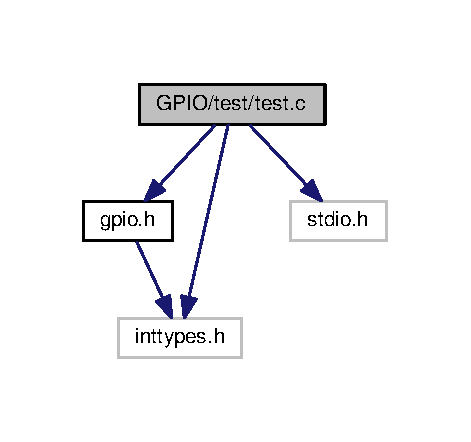
\includegraphics[width=226pt]{test_8c__incl}
\end{center}
\end{figure}
\subsection*{Funzioni}
\begin{DoxyCompactItemize}
\item 
int \hyperlink{test_8c_ae66f6b31b5ad750f1fe042a706a4e3d4}{main} ()
\end{DoxyCompactItemize}


\subsection{Documentazione delle funzioni}
\hypertarget{test_8c_ae66f6b31b5ad750f1fe042a706a4e3d4}{\index{test.\+c@{test.\+c}!main@{main}}
\index{main@{main}!test.\+c@{test.\+c}}
\subsubsection[{main}]{\setlength{\rightskip}{0pt plus 5cm}int main (
\begin{DoxyParamCaption}
{}
\end{DoxyParamCaption}
)}}\label{test_8c_ae66f6b31b5ad750f1fe042a706a4e3d4}

\hypertarget{hd44780_8c}{\section{Riferimenti per il file Lcd/hd44780.c}
\label{hd44780_8c}\index{Lcd/hd44780.\+c@{Lcd/hd44780.\+c}}
}
{\ttfamily \#include \char`\"{}hd44780.\+h\char`\"{}}\\*
{\ttfamily \#include $<$assert.\+h$>$}\\*
{\ttfamily \#include $<$stdlib.\+h$>$}\\*
Grafo delle dipendenze di inclusione per hd44780.\+c\+:\nopagebreak
\begin{figure}[H]
\begin{center}
\leavevmode
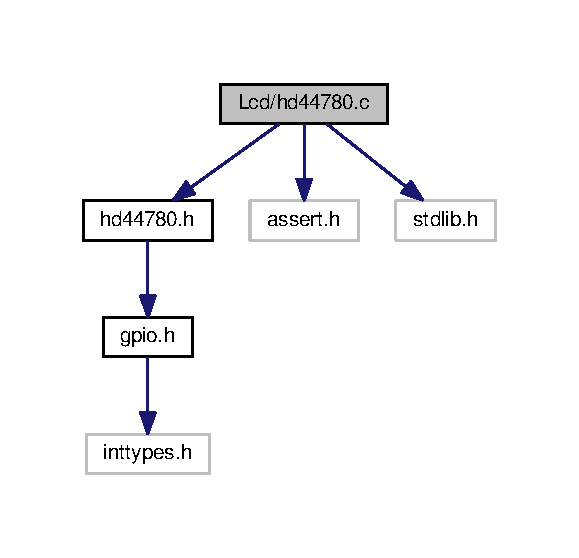
\includegraphics[width=279pt]{hd44780_8c__incl}
\end{center}
\end{figure}
\subsection*{Definizioni}
\begin{DoxyCompactItemize}
\item 
\#define \hyperlink{hd44780_8c_abc1164ac56b1a748e0ad8319be7dede8}{H\+D44780\+\_\+clear}~0x01
\item 
\#define \hyperlink{hd44780_8c_a04358db2424f9713cfb84a4fdef5b215}{H\+D44780\+\_\+home}~0x02
\item 
\#define \hyperlink{hd44780_8c_ab2681dc65568d9ec0818989aafe2eceb}{H\+D44780\+\_\+row1}~0x80
\item 
\#define \hyperlink{hd44780_8c_a7d9675a9d89c1228ada73be6239f7ef6}{H\+D44780\+\_\+row2}~0x\+C0
\item 
\#define \hyperlink{hd44780_8c_a3e52e42643f6840db3e878e23a3f82d9}{H\+D44780\+\_\+cursor\+\_\+r}~0x14
\item 
\#define \hyperlink{hd44780_8c_ad599eadde9b68b5c84f26575229383cc}{H\+D44780\+\_\+cursor\+\_\+l}~0x10
\item 
\#define \hyperlink{hd44780_8c_ab74128cead7d82100cff55cac513457a}{H\+D44780\+\_\+display\+\_\+off}~0x08
\item 
\#define \hyperlink{hd44780_8c_a05c02e143086d4d3e16c651da46357e5}{H\+D44780\+\_\+cursor\+\_\+off}~0x0\+C
\item 
\#define \hyperlink{hd44780_8c_a3967b259a0236cb4ff71b58e9e99d871}{H\+D44780\+\_\+cursor\+\_\+on}~0x0\+E
\item 
\#define \hyperlink{hd44780_8c_aee7a3931ecea03871d152b6f2fe237de}{H\+D44780\+\_\+cursor\+\_\+blink}~0x0\+F
\item 
\#define \hyperlink{hd44780_8c_abc1164ac56b1a748e0ad8319be7dede8}{H\+D44780\+\_\+clear}~0x01
\item 
\#define \hyperlink{hd44780_8c_a89582792c79342e5e196c3af6b58e813}{H\+D44780\+\_\+dec\+\_\+no\+\_\+shift}~0x04
\item 
\#define \hyperlink{hd44780_8c_a46be67bdaf1d9806e6080fc8a302e9f4}{H\+D44780\+\_\+dec\+\_\+shift}~0x05
\item 
\#define \hyperlink{hd44780_8c_a7998cf2572859cfc7a96146f9d84a8e6}{H\+D44780\+\_\+inc\+\_\+no\+\_\+shift}~0x06
\item 
\#define \hyperlink{hd44780_8c_a6c116ccd854428b9977ace77603e98f9}{H\+D44780\+\_\+inc\+\_\+shift}~0x07
\item 
\#define \hyperlink{hd44780_8c_a5f45c877d1e8266f8a2c1d0b87746950}{timer\+\_\+wait\+\_\+ms}(ms)~usleep(ms$<$$<$10)
\item 
\#define \hyperlink{hd44780_8c_a9f0a484de0de3ab1ddd77d5f716dea96}{timer\+\_\+wait\+\_\+us}(us)~usleep(us)
\item 
\#define \hyperlink{hd44780_8c_a5060e38ac985451fad57ed890aea1d77}{lcd\+\_\+command}(lcd)~\hyperlink{group__my_g_p_i_o_gab742e68093ad4c90fe299b64fd6736ca}{my\+G\+P\+I\+O\+\_\+set\+Value}(lcd-\/$>$gpio, lcd-\/$>$R\+S, \hyperlink{group__my_g_p_i_o_ggaf634fe4a0e1eab8da5000b72d6ad362ba98cde80dbda025bd1ae7231c76b55674}{my\+G\+P\+I\+O\+\_\+reset})
\item 
\#define \hyperlink{hd44780_8c_afac15d58a1ee77e8a17bc57252468ea1}{lcd\+\_\+data}(lcd)~\hyperlink{group__my_g_p_i_o_gab742e68093ad4c90fe299b64fd6736ca}{my\+G\+P\+I\+O\+\_\+set\+Value}(lcd-\/$>$gpio, lcd-\/$>$R\+S, \hyperlink{group__my_g_p_i_o_ggaf634fe4a0e1eab8da5000b72d6ad362ba10d296f3711d01189cc6c2d87f7c9149}{my\+G\+P\+I\+O\+\_\+set})
\item 
\#define \hyperlink{hd44780_8c_a7546bbb2f97e50a0469cf71934ac18e2}{lcd\+\_\+write}(lcd)~\hyperlink{group__my_g_p_i_o_gab742e68093ad4c90fe299b64fd6736ca}{my\+G\+P\+I\+O\+\_\+set\+Value}(lcd-\/$>$gpio, lcd-\/$>$R\+W, \hyperlink{group__my_g_p_i_o_ggaf634fe4a0e1eab8da5000b72d6ad362ba98cde80dbda025bd1ae7231c76b55674}{my\+G\+P\+I\+O\+\_\+reset})
\item 
\#define \hyperlink{hd44780_8c_ad7be3fdeebf9b76a774a6c1afa7fa3c8}{lcd\+\_\+read}(lcd)~\hyperlink{group__my_g_p_i_o_gab742e68093ad4c90fe299b64fd6736ca}{my\+G\+P\+I\+O\+\_\+set\+Value}(lcd-\/$>$gpio, lcd-\/$>$R\+W, \hyperlink{group__my_g_p_i_o_ggaf634fe4a0e1eab8da5000b72d6ad362ba10d296f3711d01189cc6c2d87f7c9149}{my\+G\+P\+I\+O\+\_\+set})
\item 
\#define \hyperlink{hd44780_8c_acd814f8ff18cac325b1f9f5957dd3846}{lcd\+\_\+enable}(lcd)
\end{DoxyCompactItemize}
\subsection*{Funzioni}
\begin{DoxyCompactItemize}
\item 
void \hyperlink{hd44780_8c_acc20a0564ce460f33fc998f18dd9f345}{H\+D44780\+\_\+\+Set\+Byte} (\hyperlink{struct_h_d44780___l_c_d__t}{H\+D44780\+\_\+\+L\+C\+D\+\_\+t} $\ast$lcd, uint8\+\_\+t byte)
\item 
void \hyperlink{hd44780_8c_ae12ebf4e3dd52b7d10f155e0dd1b4898}{H\+D44780\+\_\+\+Write\+Command} (\hyperlink{struct_h_d44780___l_c_d__t}{H\+D44780\+\_\+\+L\+C\+D\+\_\+t} $\ast$lcd, uint8\+\_\+t command)
\item 
void \hyperlink{hd44780_8c_a39e7e22ae76f1eec9aaf0933af398f4b}{H\+D44780\+\_\+\+Write\+Data} (\hyperlink{struct_h_d44780___l_c_d__t}{H\+D44780\+\_\+\+L\+C\+D\+\_\+t} $\ast$lcd, uint8\+\_\+t data)
\item 
int \hyperlink{hd44780_8c_ad3c60edaac713488ecb9c7ed73854a3c}{H\+D44780\+\_\+\+Validate\+Pair} (\hyperlink{struct_h_d44780___l_c_d__t}{H\+D44780\+\_\+\+L\+C\+D\+\_\+t} $\ast$lcd)
\item 
void \hyperlink{hd44780_8c_ad4120d3a2df038c193d043f386fdb221}{H\+D44780\+\_\+\+Configure\+Pin} (\hyperlink{struct_h_d44780___l_c_d__t}{H\+D44780\+\_\+\+L\+C\+D\+\_\+t} $\ast$lcd)
\item 
void \hyperlink{group___h_d44780_gad212907e20316f4fc0e93d7c7a8f338e}{H\+D44780\+\_\+\+Init8} (\hyperlink{struct_h_d44780___l_c_d__t}{H\+D44780\+\_\+\+L\+C\+D\+\_\+t} $\ast$lcd, \hyperlink{structmy_g_p_i_o__t}{my\+G\+P\+I\+O\+\_\+t} $\ast$gpio, \hyperlink{group__my_g_p_i_o_ga402a0d20afc0cb7c25554b8b023f4253}{my\+G\+P\+I\+O\+\_\+mask} R\+S, \hyperlink{group__my_g_p_i_o_ga402a0d20afc0cb7c25554b8b023f4253}{my\+G\+P\+I\+O\+\_\+mask} R\+W, \hyperlink{group__my_g_p_i_o_ga402a0d20afc0cb7c25554b8b023f4253}{my\+G\+P\+I\+O\+\_\+mask} E, \hyperlink{group__my_g_p_i_o_ga402a0d20afc0cb7c25554b8b023f4253}{my\+G\+P\+I\+O\+\_\+mask} Data7, \hyperlink{group__my_g_p_i_o_ga402a0d20afc0cb7c25554b8b023f4253}{my\+G\+P\+I\+O\+\_\+mask} Data6, \hyperlink{group__my_g_p_i_o_ga402a0d20afc0cb7c25554b8b023f4253}{my\+G\+P\+I\+O\+\_\+mask} Data5, \hyperlink{group__my_g_p_i_o_ga402a0d20afc0cb7c25554b8b023f4253}{my\+G\+P\+I\+O\+\_\+mask} Data4, \hyperlink{group__my_g_p_i_o_ga402a0d20afc0cb7c25554b8b023f4253}{my\+G\+P\+I\+O\+\_\+mask} Data3, \hyperlink{group__my_g_p_i_o_ga402a0d20afc0cb7c25554b8b023f4253}{my\+G\+P\+I\+O\+\_\+mask} Data2, \hyperlink{group__my_g_p_i_o_ga402a0d20afc0cb7c25554b8b023f4253}{my\+G\+P\+I\+O\+\_\+mask} Data1, \hyperlink{group__my_g_p_i_o_ga402a0d20afc0cb7c25554b8b023f4253}{my\+G\+P\+I\+O\+\_\+mask} Data0)
\begin{DoxyCompactList}\small\item\em Inizializza un display lcd H\+D44780 con interfacciamento ad 8 bit. \end{DoxyCompactList}\item 
void \hyperlink{group___h_d44780_ga0c08f9e41d770ebfa4af385a56b47b81}{H\+D44780\+\_\+\+Init4} (\hyperlink{struct_h_d44780___l_c_d__t}{H\+D44780\+\_\+\+L\+C\+D\+\_\+t} $\ast$lcd, \hyperlink{structmy_g_p_i_o__t}{my\+G\+P\+I\+O\+\_\+t} $\ast$gpio, \hyperlink{group__my_g_p_i_o_ga402a0d20afc0cb7c25554b8b023f4253}{my\+G\+P\+I\+O\+\_\+mask} R\+S, \hyperlink{group__my_g_p_i_o_ga402a0d20afc0cb7c25554b8b023f4253}{my\+G\+P\+I\+O\+\_\+mask} R\+W, \hyperlink{group__my_g_p_i_o_ga402a0d20afc0cb7c25554b8b023f4253}{my\+G\+P\+I\+O\+\_\+mask} E, \hyperlink{group__my_g_p_i_o_ga402a0d20afc0cb7c25554b8b023f4253}{my\+G\+P\+I\+O\+\_\+mask} Data7, \hyperlink{group__my_g_p_i_o_ga402a0d20afc0cb7c25554b8b023f4253}{my\+G\+P\+I\+O\+\_\+mask} Data6, \hyperlink{group__my_g_p_i_o_ga402a0d20afc0cb7c25554b8b023f4253}{my\+G\+P\+I\+O\+\_\+mask} Data5, \hyperlink{group__my_g_p_i_o_ga402a0d20afc0cb7c25554b8b023f4253}{my\+G\+P\+I\+O\+\_\+mask} Data4)
\begin{DoxyCompactList}\small\item\em Inizializza un oggetto display lcd H\+D44780 affinche' si utilizzi l'interfaccia a 4 bit. \end{DoxyCompactList}\item 
void \hyperlink{group___h_d44780_ga57b8c6ca0b3c12e5f7273b3c373a6f17}{H\+D44780\+\_\+\+Printc} (\hyperlink{struct_h_d44780___l_c_d__t}{H\+D44780\+\_\+\+L\+C\+D\+\_\+t} $\ast$lcd, char c)
\begin{DoxyCompactList}\small\item\em Stampa un carattere. \end{DoxyCompactList}\item 
void \hyperlink{group___h_d44780_ga3aedff8e2040e62db569fde955d3987b}{H\+D44780\+\_\+\+Print} (\hyperlink{struct_h_d44780___l_c_d__t}{H\+D44780\+\_\+\+L\+C\+D\+\_\+t} $\ast$lcd, const char $\ast$s)
\begin{DoxyCompactList}\small\item\em Stampa una stringa null-\/terminated di caratteri. \end{DoxyCompactList}\item 
void \hyperlink{group___h_d44780_ga2a5d4d528175321c46c790b581959e63}{H\+D44780\+\_\+print\+Binary8} (\hyperlink{struct_h_d44780___l_c_d__t}{H\+D44780\+\_\+\+L\+C\+D\+\_\+t} $\ast$lcd, uint8\+\_\+t b)
\begin{DoxyCompactList}\small\item\em Stampa un byte in binario. (bit piu' significativo a sinistra) \end{DoxyCompactList}\item 
void \hyperlink{group___h_d44780_ga95cceef2401c5519295e5a83c6688b5c}{H\+D44780\+\_\+print\+Binary32} (\hyperlink{struct_h_d44780___l_c_d__t}{H\+D44780\+\_\+\+L\+C\+D\+\_\+t} $\ast$lcd, uint32\+\_\+t w)
\begin{DoxyCompactList}\small\item\em Stampa una word di 32 bit in binario. (bit piu' significativo a sinistra) \end{DoxyCompactList}\item 
void \hyperlink{group___h_d44780_ga0f99bc5458acb172d0f3bfeb94f90e2a}{H\+D44780\+\_\+print\+Binary64} (\hyperlink{struct_h_d44780___l_c_d__t}{H\+D44780\+\_\+\+L\+C\+D\+\_\+t} $\ast$lcd, uint64\+\_\+t b)
\begin{DoxyCompactList}\small\item\em Stampa un blocco di 64 bit in binario. (bit piu' significativo a sinistra) \end{DoxyCompactList}\item 
void \hyperlink{group___h_d44780_gad967bd458b4d2bd358a93cbb7144addd}{H\+D44780\+\_\+print\+Hex8} (\hyperlink{struct_h_d44780___l_c_d__t}{H\+D44780\+\_\+\+L\+C\+D\+\_\+t} $\ast$lcd, uint8\+\_\+t b)
\begin{DoxyCompactList}\small\item\em Stampa un byte in esadecimale. (bit piu' significativo a sinistra) \end{DoxyCompactList}\item 
void \hyperlink{group___h_d44780_gaa82a2a27a3008f55c969a2d390c50497}{H\+D44780\+\_\+print\+Hex32} (\hyperlink{struct_h_d44780___l_c_d__t}{H\+D44780\+\_\+\+L\+C\+D\+\_\+t} $\ast$lcd, uint32\+\_\+t w)
\begin{DoxyCompactList}\small\item\em Stampa una word di 32 bit in esadecimale. (bit piu' significativo a sinistra) \end{DoxyCompactList}\item 
void \hyperlink{group___h_d44780_ga7a4b110e7da806f8c01e01d184d3a19a}{H\+D44780\+\_\+print\+Hex64} (\hyperlink{struct_h_d44780___l_c_d__t}{H\+D44780\+\_\+\+L\+C\+D\+\_\+t} $\ast$lcd, uint64\+\_\+t b)
\begin{DoxyCompactList}\small\item\em Stampa un blocco di 64 bit in esadecimale. (bit piu' significativo a sinistra) \end{DoxyCompactList}\item 
void \hyperlink{group___h_d44780_ga38cac13d7a66f068be54f79a716ff7d4}{H\+D44780\+\_\+\+Clear} (\hyperlink{struct_h_d44780___l_c_d__t}{H\+D44780\+\_\+\+L\+C\+D\+\_\+t} $\ast$lcd)
\begin{DoxyCompactList}\small\item\em Pulisce il display e sposta il cursore all'inizio della prima riga. \end{DoxyCompactList}\item 
void \hyperlink{group___h_d44780_ga68e3712332aa9482d4bdaa4991a92127}{H\+D44780\+\_\+\+Home} (\hyperlink{struct_h_d44780___l_c_d__t}{H\+D44780\+\_\+\+L\+C\+D\+\_\+t} $\ast$lcd)
\begin{DoxyCompactList}\small\item\em Sposta il cursore all'inizio della prima riga. \end{DoxyCompactList}\item 
void \hyperlink{group___h_d44780_gad90e2924a4e632ce42940323f8f49e37}{H\+D44780\+\_\+\+Move\+To\+Row1} (\hyperlink{struct_h_d44780___l_c_d__t}{H\+D44780\+\_\+\+L\+C\+D\+\_\+t} $\ast$lcd)
\begin{DoxyCompactList}\small\item\em Sposta il cursore all'inizio della prima riga. \end{DoxyCompactList}\item 
void \hyperlink{group___h_d44780_ga713670d498b6f5d50a174df19081c515}{H\+D44780\+\_\+\+Move\+To\+Row2} (\hyperlink{struct_h_d44780___l_c_d__t}{H\+D44780\+\_\+\+L\+C\+D\+\_\+t} $\ast$lcd)
\begin{DoxyCompactList}\small\item\em Sposta il cursore all'inizio della seconda riga. \end{DoxyCompactList}\item 
void \hyperlink{group___h_d44780_gabcea9a03050c46530e39b7556c673baf}{H\+D44780\+\_\+\+Move\+Cursor} (\hyperlink{struct_h_d44780___l_c_d__t}{H\+D44780\+\_\+\+L\+C\+D\+\_\+t} $\ast$lcd, \hyperlink{group___h_d44780_gaf46f4db4f981d3a1088804a6d6980d30}{H\+D44780\+\_\+\+Direction\+\_\+t} dir)
\begin{DoxyCompactList}\small\item\em Sposta il cursore di una posizione a destra o sinistra. \end{DoxyCompactList}\item 
void \hyperlink{group___h_d44780_ga5cf07b2179272029410f9a81f56621ed}{H\+D44780\+\_\+\+Display\+Off} (\hyperlink{struct_h_d44780___l_c_d__t}{H\+D44780\+\_\+\+L\+C\+D\+\_\+t} $\ast$lcd)
\begin{DoxyCompactList}\small\item\em Disattiva il display. \end{DoxyCompactList}\item 
void \hyperlink{group___h_d44780_ga56421dc398825188aa10257063a3ee4b}{H\+D44780\+\_\+\+Cursor\+Off} (\hyperlink{struct_h_d44780___l_c_d__t}{H\+D44780\+\_\+\+L\+C\+D\+\_\+t} $\ast$lcd)
\begin{DoxyCompactList}\small\item\em Disattiva la visualizzazione del cursore. \end{DoxyCompactList}\item 
void \hyperlink{group___h_d44780_ga3a381cb44df5d76d79be5ed71a52bae6}{H\+D44780\+\_\+\+Cursor\+On} (\hyperlink{struct_h_d44780___l_c_d__t}{H\+D44780\+\_\+\+L\+C\+D\+\_\+t} $\ast$lcd)
\begin{DoxyCompactList}\small\item\em Attiva la visualizzazione del cursore. \end{DoxyCompactList}\item 
void \hyperlink{group___h_d44780_ga92eb58cb7d73c9a87b7087a9c56f73d5}{H\+D44780\+\_\+\+Cursor\+Blink} (\hyperlink{struct_h_d44780___l_c_d__t}{H\+D44780\+\_\+\+L\+C\+D\+\_\+t} $\ast$lcd)
\begin{DoxyCompactList}\small\item\em Attiva il cursore lampeggiante. \end{DoxyCompactList}\end{DoxyCompactItemize}


\subsection{Descrizione dettagliata}
\begin{DoxyAuthor}{Autore}
Salvatore Barone \href{mailto:salvator.barone@gmail.com}{\tt salvator.\+barone@gmail.\+com}
\end{DoxyAuthor}
\begin{DoxyCopyright}{Copyright}
Copyright 2017 Salvatore Barone \href{mailto:salvator.barone@gmail.com}{\tt salvator.\+barone@gmail.\+com}
\end{DoxyCopyright}
This file is part of Zynq7000\+Driver\+Pack

Zynq7000\+Driver\+Pack is free software; you can redistribute it and/or modify it under the terms of the G\+N\+U General Public License as published by the Free Software Foundation; either version 3 of the License, or any later version.

Zynq7000\+Driver\+Pack is distributed in the hope that it will be useful, but W\+I\+T\+H\+O\+U\+T A\+N\+Y W\+A\+R\+R\+A\+N\+T\+Y; without even the implied warranty of M\+E\+R\+C\+H\+A\+N\+T\+A\+B\+I\+L\+I\+T\+Y or F\+I\+T\+N\+E\+S\+S F\+O\+R A P\+A\+R\+T\+I\+C\+U\+L\+A\+R P\+U\+R\+P\+O\+S\+E. See the G\+N\+U General Public License for more details.

You should have received a copy of the G\+N\+U General Public License along with this program; if not, write to the Free Software Foundation, Inc., 51 Franklin Street, Fifth Floor, Boston, M\+A 02110-\/1301, U\+S\+A. 

\subsection{Documentazione delle definizioni}
\hypertarget{hd44780_8c_abc1164ac56b1a748e0ad8319be7dede8}{\index{hd44780.\+c@{hd44780.\+c}!H\+D44780\+\_\+clear@{H\+D44780\+\_\+clear}}
\index{H\+D44780\+\_\+clear@{H\+D44780\+\_\+clear}!hd44780.\+c@{hd44780.\+c}}
\subsubsection[{H\+D44780\+\_\+clear}]{\setlength{\rightskip}{0pt plus 5cm}\#define H\+D44780\+\_\+clear~0x01}}\label{hd44780_8c_abc1164ac56b1a748e0ad8319be7dede8}
\hypertarget{hd44780_8c_abc1164ac56b1a748e0ad8319be7dede8}{\index{hd44780.\+c@{hd44780.\+c}!H\+D44780\+\_\+clear@{H\+D44780\+\_\+clear}}
\index{H\+D44780\+\_\+clear@{H\+D44780\+\_\+clear}!hd44780.\+c@{hd44780.\+c}}
\subsubsection[{H\+D44780\+\_\+clear}]{\setlength{\rightskip}{0pt plus 5cm}\#define H\+D44780\+\_\+clear~0x01}}\label{hd44780_8c_abc1164ac56b1a748e0ad8319be7dede8}
\hypertarget{hd44780_8c_aee7a3931ecea03871d152b6f2fe237de}{\index{hd44780.\+c@{hd44780.\+c}!H\+D44780\+\_\+cursor\+\_\+blink@{H\+D44780\+\_\+cursor\+\_\+blink}}
\index{H\+D44780\+\_\+cursor\+\_\+blink@{H\+D44780\+\_\+cursor\+\_\+blink}!hd44780.\+c@{hd44780.\+c}}
\subsubsection[{H\+D44780\+\_\+cursor\+\_\+blink}]{\setlength{\rightskip}{0pt plus 5cm}\#define H\+D44780\+\_\+cursor\+\_\+blink~0x0\+F}}\label{hd44780_8c_aee7a3931ecea03871d152b6f2fe237de}
\hypertarget{hd44780_8c_ad599eadde9b68b5c84f26575229383cc}{\index{hd44780.\+c@{hd44780.\+c}!H\+D44780\+\_\+cursor\+\_\+l@{H\+D44780\+\_\+cursor\+\_\+l}}
\index{H\+D44780\+\_\+cursor\+\_\+l@{H\+D44780\+\_\+cursor\+\_\+l}!hd44780.\+c@{hd44780.\+c}}
\subsubsection[{H\+D44780\+\_\+cursor\+\_\+l}]{\setlength{\rightskip}{0pt plus 5cm}\#define H\+D44780\+\_\+cursor\+\_\+l~0x10}}\label{hd44780_8c_ad599eadde9b68b5c84f26575229383cc}
\hypertarget{hd44780_8c_a05c02e143086d4d3e16c651da46357e5}{\index{hd44780.\+c@{hd44780.\+c}!H\+D44780\+\_\+cursor\+\_\+off@{H\+D44780\+\_\+cursor\+\_\+off}}
\index{H\+D44780\+\_\+cursor\+\_\+off@{H\+D44780\+\_\+cursor\+\_\+off}!hd44780.\+c@{hd44780.\+c}}
\subsubsection[{H\+D44780\+\_\+cursor\+\_\+off}]{\setlength{\rightskip}{0pt plus 5cm}\#define H\+D44780\+\_\+cursor\+\_\+off~0x0\+C}}\label{hd44780_8c_a05c02e143086d4d3e16c651da46357e5}
\hypertarget{hd44780_8c_a3967b259a0236cb4ff71b58e9e99d871}{\index{hd44780.\+c@{hd44780.\+c}!H\+D44780\+\_\+cursor\+\_\+on@{H\+D44780\+\_\+cursor\+\_\+on}}
\index{H\+D44780\+\_\+cursor\+\_\+on@{H\+D44780\+\_\+cursor\+\_\+on}!hd44780.\+c@{hd44780.\+c}}
\subsubsection[{H\+D44780\+\_\+cursor\+\_\+on}]{\setlength{\rightskip}{0pt plus 5cm}\#define H\+D44780\+\_\+cursor\+\_\+on~0x0\+E}}\label{hd44780_8c_a3967b259a0236cb4ff71b58e9e99d871}
\hypertarget{hd44780_8c_a3e52e42643f6840db3e878e23a3f82d9}{\index{hd44780.\+c@{hd44780.\+c}!H\+D44780\+\_\+cursor\+\_\+r@{H\+D44780\+\_\+cursor\+\_\+r}}
\index{H\+D44780\+\_\+cursor\+\_\+r@{H\+D44780\+\_\+cursor\+\_\+r}!hd44780.\+c@{hd44780.\+c}}
\subsubsection[{H\+D44780\+\_\+cursor\+\_\+r}]{\setlength{\rightskip}{0pt plus 5cm}\#define H\+D44780\+\_\+cursor\+\_\+r~0x14}}\label{hd44780_8c_a3e52e42643f6840db3e878e23a3f82d9}
\hypertarget{hd44780_8c_a89582792c79342e5e196c3af6b58e813}{\index{hd44780.\+c@{hd44780.\+c}!H\+D44780\+\_\+dec\+\_\+no\+\_\+shift@{H\+D44780\+\_\+dec\+\_\+no\+\_\+shift}}
\index{H\+D44780\+\_\+dec\+\_\+no\+\_\+shift@{H\+D44780\+\_\+dec\+\_\+no\+\_\+shift}!hd44780.\+c@{hd44780.\+c}}
\subsubsection[{H\+D44780\+\_\+dec\+\_\+no\+\_\+shift}]{\setlength{\rightskip}{0pt plus 5cm}\#define H\+D44780\+\_\+dec\+\_\+no\+\_\+shift~0x04}}\label{hd44780_8c_a89582792c79342e5e196c3af6b58e813}
\hypertarget{hd44780_8c_a46be67bdaf1d9806e6080fc8a302e9f4}{\index{hd44780.\+c@{hd44780.\+c}!H\+D44780\+\_\+dec\+\_\+shift@{H\+D44780\+\_\+dec\+\_\+shift}}
\index{H\+D44780\+\_\+dec\+\_\+shift@{H\+D44780\+\_\+dec\+\_\+shift}!hd44780.\+c@{hd44780.\+c}}
\subsubsection[{H\+D44780\+\_\+dec\+\_\+shift}]{\setlength{\rightskip}{0pt plus 5cm}\#define H\+D44780\+\_\+dec\+\_\+shift~0x05}}\label{hd44780_8c_a46be67bdaf1d9806e6080fc8a302e9f4}
\hypertarget{hd44780_8c_ab74128cead7d82100cff55cac513457a}{\index{hd44780.\+c@{hd44780.\+c}!H\+D44780\+\_\+display\+\_\+off@{H\+D44780\+\_\+display\+\_\+off}}
\index{H\+D44780\+\_\+display\+\_\+off@{H\+D44780\+\_\+display\+\_\+off}!hd44780.\+c@{hd44780.\+c}}
\subsubsection[{H\+D44780\+\_\+display\+\_\+off}]{\setlength{\rightskip}{0pt plus 5cm}\#define H\+D44780\+\_\+display\+\_\+off~0x08}}\label{hd44780_8c_ab74128cead7d82100cff55cac513457a}
\hypertarget{hd44780_8c_a04358db2424f9713cfb84a4fdef5b215}{\index{hd44780.\+c@{hd44780.\+c}!H\+D44780\+\_\+home@{H\+D44780\+\_\+home}}
\index{H\+D44780\+\_\+home@{H\+D44780\+\_\+home}!hd44780.\+c@{hd44780.\+c}}
\subsubsection[{H\+D44780\+\_\+home}]{\setlength{\rightskip}{0pt plus 5cm}\#define H\+D44780\+\_\+home~0x02}}\label{hd44780_8c_a04358db2424f9713cfb84a4fdef5b215}
\hypertarget{hd44780_8c_a7998cf2572859cfc7a96146f9d84a8e6}{\index{hd44780.\+c@{hd44780.\+c}!H\+D44780\+\_\+inc\+\_\+no\+\_\+shift@{H\+D44780\+\_\+inc\+\_\+no\+\_\+shift}}
\index{H\+D44780\+\_\+inc\+\_\+no\+\_\+shift@{H\+D44780\+\_\+inc\+\_\+no\+\_\+shift}!hd44780.\+c@{hd44780.\+c}}
\subsubsection[{H\+D44780\+\_\+inc\+\_\+no\+\_\+shift}]{\setlength{\rightskip}{0pt plus 5cm}\#define H\+D44780\+\_\+inc\+\_\+no\+\_\+shift~0x06}}\label{hd44780_8c_a7998cf2572859cfc7a96146f9d84a8e6}
\hypertarget{hd44780_8c_a6c116ccd854428b9977ace77603e98f9}{\index{hd44780.\+c@{hd44780.\+c}!H\+D44780\+\_\+inc\+\_\+shift@{H\+D44780\+\_\+inc\+\_\+shift}}
\index{H\+D44780\+\_\+inc\+\_\+shift@{H\+D44780\+\_\+inc\+\_\+shift}!hd44780.\+c@{hd44780.\+c}}
\subsubsection[{H\+D44780\+\_\+inc\+\_\+shift}]{\setlength{\rightskip}{0pt plus 5cm}\#define H\+D44780\+\_\+inc\+\_\+shift~0x07}}\label{hd44780_8c_a6c116ccd854428b9977ace77603e98f9}
\hypertarget{hd44780_8c_ab2681dc65568d9ec0818989aafe2eceb}{\index{hd44780.\+c@{hd44780.\+c}!H\+D44780\+\_\+row1@{H\+D44780\+\_\+row1}}
\index{H\+D44780\+\_\+row1@{H\+D44780\+\_\+row1}!hd44780.\+c@{hd44780.\+c}}
\subsubsection[{H\+D44780\+\_\+row1}]{\setlength{\rightskip}{0pt plus 5cm}\#define H\+D44780\+\_\+row1~0x80}}\label{hd44780_8c_ab2681dc65568d9ec0818989aafe2eceb}
\hypertarget{hd44780_8c_a7d9675a9d89c1228ada73be6239f7ef6}{\index{hd44780.\+c@{hd44780.\+c}!H\+D44780\+\_\+row2@{H\+D44780\+\_\+row2}}
\index{H\+D44780\+\_\+row2@{H\+D44780\+\_\+row2}!hd44780.\+c@{hd44780.\+c}}
\subsubsection[{H\+D44780\+\_\+row2}]{\setlength{\rightskip}{0pt plus 5cm}\#define H\+D44780\+\_\+row2~0x\+C0}}\label{hd44780_8c_a7d9675a9d89c1228ada73be6239f7ef6}
\hypertarget{hd44780_8c_a5060e38ac985451fad57ed890aea1d77}{\index{hd44780.\+c@{hd44780.\+c}!lcd\+\_\+command@{lcd\+\_\+command}}
\index{lcd\+\_\+command@{lcd\+\_\+command}!hd44780.\+c@{hd44780.\+c}}
\subsubsection[{lcd\+\_\+command}]{\setlength{\rightskip}{0pt plus 5cm}\#define lcd\+\_\+command(
\begin{DoxyParamCaption}
\item[{}]{lcd}
\end{DoxyParamCaption}
)~{\bf my\+G\+P\+I\+O\+\_\+set\+Value}(lcd-\/$>$gpio, lcd-\/$>$R\+S, {\bf my\+G\+P\+I\+O\+\_\+reset})}}\label{hd44780_8c_a5060e38ac985451fad57ed890aea1d77}
\hypertarget{hd44780_8c_afac15d58a1ee77e8a17bc57252468ea1}{\index{hd44780.\+c@{hd44780.\+c}!lcd\+\_\+data@{lcd\+\_\+data}}
\index{lcd\+\_\+data@{lcd\+\_\+data}!hd44780.\+c@{hd44780.\+c}}
\subsubsection[{lcd\+\_\+data}]{\setlength{\rightskip}{0pt plus 5cm}\#define lcd\+\_\+data(
\begin{DoxyParamCaption}
\item[{}]{lcd}
\end{DoxyParamCaption}
)~{\bf my\+G\+P\+I\+O\+\_\+set\+Value}(lcd-\/$>$gpio, lcd-\/$>$R\+S, {\bf my\+G\+P\+I\+O\+\_\+set})}}\label{hd44780_8c_afac15d58a1ee77e8a17bc57252468ea1}
\hypertarget{hd44780_8c_acd814f8ff18cac325b1f9f5957dd3846}{\index{hd44780.\+c@{hd44780.\+c}!lcd\+\_\+enable@{lcd\+\_\+enable}}
\index{lcd\+\_\+enable@{lcd\+\_\+enable}!hd44780.\+c@{hd44780.\+c}}
\subsubsection[{lcd\+\_\+enable}]{\setlength{\rightskip}{0pt plus 5cm}\#define lcd\+\_\+enable(
\begin{DoxyParamCaption}
\item[{}]{lcd}
\end{DoxyParamCaption}
)}}\label{hd44780_8c_acd814f8ff18cac325b1f9f5957dd3846}
{\bfseries Valore\+:}
\begin{DoxyCode}
\hyperlink{group__my_g_p_i_o_gab742e68093ad4c90fe299b64fd6736ca}{myGPIO\_setValue}(lcd->gpio, lcd->E, \hyperlink{group__my_g_p_i_o_ggaf634fe4a0e1eab8da5000b72d6ad362ba10d296f3711d01189cc6c2d87f7c9149}{myGPIO\_set}); \hyperlink{hd44780_8c_a9f0a484de0de3ab1ddd77d5f716dea96}{\(\backslash\)}
\hyperlink{hd44780_8c_a9f0a484de0de3ab1ddd77d5f716dea96}{                            timer\_wait\_us}(100); \hyperlink{group__my_g_p_i_o_gab742e68093ad4c90fe299b64fd6736ca}{\(\backslash\)}
\hyperlink{group__my_g_p_i_o_gab742e68093ad4c90fe299b64fd6736ca}{                            myGPIO\_setValue}(lcd->gpio, lcd->E, 
      \hyperlink{group__my_g_p_i_o_ggaf634fe4a0e1eab8da5000b72d6ad362ba98cde80dbda025bd1ae7231c76b55674}{myGPIO\_reset})
\end{DoxyCode}
\hypertarget{hd44780_8c_ad7be3fdeebf9b76a774a6c1afa7fa3c8}{\index{hd44780.\+c@{hd44780.\+c}!lcd\+\_\+read@{lcd\+\_\+read}}
\index{lcd\+\_\+read@{lcd\+\_\+read}!hd44780.\+c@{hd44780.\+c}}
\subsubsection[{lcd\+\_\+read}]{\setlength{\rightskip}{0pt plus 5cm}\#define lcd\+\_\+read(
\begin{DoxyParamCaption}
\item[{}]{lcd}
\end{DoxyParamCaption}
)~{\bf my\+G\+P\+I\+O\+\_\+set\+Value}(lcd-\/$>$gpio, lcd-\/$>$R\+W, {\bf my\+G\+P\+I\+O\+\_\+set})}}\label{hd44780_8c_ad7be3fdeebf9b76a774a6c1afa7fa3c8}
\hypertarget{hd44780_8c_a7546bbb2f97e50a0469cf71934ac18e2}{\index{hd44780.\+c@{hd44780.\+c}!lcd\+\_\+write@{lcd\+\_\+write}}
\index{lcd\+\_\+write@{lcd\+\_\+write}!hd44780.\+c@{hd44780.\+c}}
\subsubsection[{lcd\+\_\+write}]{\setlength{\rightskip}{0pt plus 5cm}\#define lcd\+\_\+write(
\begin{DoxyParamCaption}
\item[{}]{lcd}
\end{DoxyParamCaption}
)~{\bf my\+G\+P\+I\+O\+\_\+set\+Value}(lcd-\/$>$gpio, lcd-\/$>$R\+W, {\bf my\+G\+P\+I\+O\+\_\+reset})}}\label{hd44780_8c_a7546bbb2f97e50a0469cf71934ac18e2}
\hypertarget{hd44780_8c_a5f45c877d1e8266f8a2c1d0b87746950}{\index{hd44780.\+c@{hd44780.\+c}!timer\+\_\+wait\+\_\+ms@{timer\+\_\+wait\+\_\+ms}}
\index{timer\+\_\+wait\+\_\+ms@{timer\+\_\+wait\+\_\+ms}!hd44780.\+c@{hd44780.\+c}}
\subsubsection[{timer\+\_\+wait\+\_\+ms}]{\setlength{\rightskip}{0pt plus 5cm}\#define timer\+\_\+wait\+\_\+ms(
\begin{DoxyParamCaption}
\item[{}]{ms}
\end{DoxyParamCaption}
)~usleep(ms$<$$<$10)}}\label{hd44780_8c_a5f45c877d1e8266f8a2c1d0b87746950}
\hypertarget{hd44780_8c_a9f0a484de0de3ab1ddd77d5f716dea96}{\index{hd44780.\+c@{hd44780.\+c}!timer\+\_\+wait\+\_\+us@{timer\+\_\+wait\+\_\+us}}
\index{timer\+\_\+wait\+\_\+us@{timer\+\_\+wait\+\_\+us}!hd44780.\+c@{hd44780.\+c}}
\subsubsection[{timer\+\_\+wait\+\_\+us}]{\setlength{\rightskip}{0pt plus 5cm}\#define timer\+\_\+wait\+\_\+us(
\begin{DoxyParamCaption}
\item[{}]{us}
\end{DoxyParamCaption}
)~usleep(us)}}\label{hd44780_8c_a9f0a484de0de3ab1ddd77d5f716dea96}


\subsection{Documentazione delle funzioni}
\hypertarget{hd44780_8c_ad4120d3a2df038c193d043f386fdb221}{\index{hd44780.\+c@{hd44780.\+c}!H\+D44780\+\_\+\+Configure\+Pin@{H\+D44780\+\_\+\+Configure\+Pin}}
\index{H\+D44780\+\_\+\+Configure\+Pin@{H\+D44780\+\_\+\+Configure\+Pin}!hd44780.\+c@{hd44780.\+c}}
\subsubsection[{H\+D44780\+\_\+\+Configure\+Pin}]{\setlength{\rightskip}{0pt plus 5cm}void H\+D44780\+\_\+\+Configure\+Pin (
\begin{DoxyParamCaption}
\item[{{\bf H\+D44780\+\_\+\+L\+C\+D\+\_\+t} $\ast$}]{lcd}
\end{DoxyParamCaption}
)}}\label{hd44780_8c_ad4120d3a2df038c193d043f386fdb221}
\hypertarget{hd44780_8c_acc20a0564ce460f33fc998f18dd9f345}{\index{hd44780.\+c@{hd44780.\+c}!H\+D44780\+\_\+\+Set\+Byte@{H\+D44780\+\_\+\+Set\+Byte}}
\index{H\+D44780\+\_\+\+Set\+Byte@{H\+D44780\+\_\+\+Set\+Byte}!hd44780.\+c@{hd44780.\+c}}
\subsubsection[{H\+D44780\+\_\+\+Set\+Byte}]{\setlength{\rightskip}{0pt plus 5cm}void H\+D44780\+\_\+\+Set\+Byte (
\begin{DoxyParamCaption}
\item[{{\bf H\+D44780\+\_\+\+L\+C\+D\+\_\+t} $\ast$}]{lcd, }
\item[{uint8\+\_\+t}]{byte}
\end{DoxyParamCaption}
)}}\label{hd44780_8c_acc20a0564ce460f33fc998f18dd9f345}
\hypertarget{hd44780_8c_ad3c60edaac713488ecb9c7ed73854a3c}{\index{hd44780.\+c@{hd44780.\+c}!H\+D44780\+\_\+\+Validate\+Pair@{H\+D44780\+\_\+\+Validate\+Pair}}
\index{H\+D44780\+\_\+\+Validate\+Pair@{H\+D44780\+\_\+\+Validate\+Pair}!hd44780.\+c@{hd44780.\+c}}
\subsubsection[{H\+D44780\+\_\+\+Validate\+Pair}]{\setlength{\rightskip}{0pt plus 5cm}int H\+D44780\+\_\+\+Validate\+Pair (
\begin{DoxyParamCaption}
\item[{{\bf H\+D44780\+\_\+\+L\+C\+D\+\_\+t} $\ast$}]{lcd}
\end{DoxyParamCaption}
)}}\label{hd44780_8c_ad3c60edaac713488ecb9c7ed73854a3c}
\hypertarget{hd44780_8c_ae12ebf4e3dd52b7d10f155e0dd1b4898}{\index{hd44780.\+c@{hd44780.\+c}!H\+D44780\+\_\+\+Write\+Command@{H\+D44780\+\_\+\+Write\+Command}}
\index{H\+D44780\+\_\+\+Write\+Command@{H\+D44780\+\_\+\+Write\+Command}!hd44780.\+c@{hd44780.\+c}}
\subsubsection[{H\+D44780\+\_\+\+Write\+Command}]{\setlength{\rightskip}{0pt plus 5cm}void H\+D44780\+\_\+\+Write\+Command (
\begin{DoxyParamCaption}
\item[{{\bf H\+D44780\+\_\+\+L\+C\+D\+\_\+t} $\ast$}]{lcd, }
\item[{uint8\+\_\+t}]{command}
\end{DoxyParamCaption}
)}}\label{hd44780_8c_ae12ebf4e3dd52b7d10f155e0dd1b4898}
\hypertarget{hd44780_8c_a39e7e22ae76f1eec9aaf0933af398f4b}{\index{hd44780.\+c@{hd44780.\+c}!H\+D44780\+\_\+\+Write\+Data@{H\+D44780\+\_\+\+Write\+Data}}
\index{H\+D44780\+\_\+\+Write\+Data@{H\+D44780\+\_\+\+Write\+Data}!hd44780.\+c@{hd44780.\+c}}
\subsubsection[{H\+D44780\+\_\+\+Write\+Data}]{\setlength{\rightskip}{0pt plus 5cm}void H\+D44780\+\_\+\+Write\+Data (
\begin{DoxyParamCaption}
\item[{{\bf H\+D44780\+\_\+\+L\+C\+D\+\_\+t} $\ast$}]{lcd, }
\item[{uint8\+\_\+t}]{data}
\end{DoxyParamCaption}
)}}\label{hd44780_8c_a39e7e22ae76f1eec9aaf0933af398f4b}

\hypertarget{hd44780_8h}{\section{Riferimenti per il file Lcd/hd44780.h}
\label{hd44780_8h}\index{Lcd/hd44780.\+h@{Lcd/hd44780.\+h}}
}
{\ttfamily \#include \char`\"{}my\+G\+P\+I\+O.\+h\char`\"{}}\\*
Grafo delle dipendenze di inclusione per hd44780.\+h\+:
\nopagebreak
\begin{figure}[H]
\begin{center}
\leavevmode
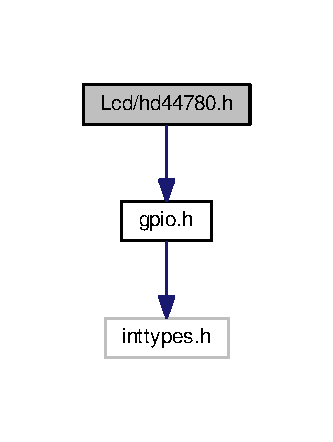
\includegraphics[width=160pt]{hd44780_8h__incl}
\end{center}
\end{figure}
Questo grafo mostra quali altri file includono direttamente o indirettamente questo file\+:\nopagebreak
\begin{figure}[H]
\begin{center}
\leavevmode
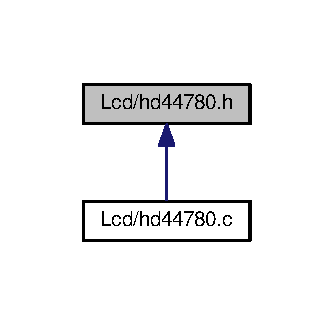
\includegraphics[width=160pt]{hd44780_8h__dep__incl}
\end{center}
\end{figure}
\subsection*{Strutture dati}
\begin{DoxyCompactItemize}
\item 
struct \hyperlink{struct_h_d44780___l_c_d__t}{H\+D44780\+\_\+\+L\+C\+D\+\_\+t}
\begin{DoxyCompactList}\small\item\em Struttura opaca che astrae un device Display L\+C\+D con cntroller Hitachi H\+D44780, o compatibile. Un oggetto di tipo \hyperlink{struct_h_d44780___l_c_d__t}{H\+D44780\+\_\+\+L\+C\+D\+\_\+t} rappresenta un device lcd H\+D44780. Il modulo e' pensato per permettere la gestione di piu' display da parte dello stesso processore, agendo su oggetti \hyperlink{struct_h_d44780___l_c_d__t}{H\+D44780\+\_\+\+L\+C\+D\+\_\+t} diversi. Il modulo permette di utilizzare sia l'interfacciamento ad otto bit che quello a quattro bit, inizializzando il device opportunamente, attraverso l'uso delle funzioni H\+D44780\+\_\+\+Init8 e\+H\+D44780\+\_\+\+Init4. Il modulo fornisce anche semplici funzioni per la stampa di un carattere o di una stringa null-\/terminated di caratteri. Si veda la documentazione delle funzioni H\+D44780\+\_\+\+Printc e H\+D44780\+\_\+\+Print. Inoltre sono presenti diverse funzioni di utilita' generica, come quelle per la pulizia del display, per lo spostamento del cursore di un posto in avanti o indietro, alla riga in basso o in alto. \end{DoxyCompactList}\end{DoxyCompactItemize}
\subsection*{Tipi enumerati (enum)}
\begin{DoxyCompactItemize}
\item 
enum \hyperlink{group___h_d44780_gaaaea8b73e24f7658da4118f6b01b45f0}{H\+D44780\+\_\+\+Interface\+Mode\+\_\+t} \{ \hyperlink{group___h_d44780_ggaaaea8b73e24f7658da4118f6b01b45f0a45bf6ce7ec7c951f692bdce9f0f485c6}{H\+D44780\+\_\+\+I\+N\+T\+E\+R\+F\+A\+C\+E\+\_\+4bit}, 
\hyperlink{group___h_d44780_ggaaaea8b73e24f7658da4118f6b01b45f0a24da9b234f9358c14184fe21f3c47de5}{H\+D44780\+\_\+\+I\+N\+T\+E\+R\+F\+A\+C\+E\+\_\+8bit}
 \}
\begin{DoxyCompactList}\small\item\em Modalita' di interfacciamento. Il modulo supporta sia interfacciamento a 4 bit che ad 8 bit. \end{DoxyCompactList}\item 
enum \hyperlink{group___h_d44780_gaf46f4db4f981d3a1088804a6d6980d30}{H\+D44780\+\_\+\+Direction\+\_\+t} \{ \hyperlink{group___h_d44780_ggaf46f4db4f981d3a1088804a6d6980d30aa4d704398d4edd1e0dec8dbb55f90292}{H\+D44780\+\_\+\+Cursor\+Left}, 
\hyperlink{group___h_d44780_ggaf46f4db4f981d3a1088804a6d6980d30a26006ced693b6bab28c6e30bfdb8c399}{H\+D44780\+\_\+\+Cursor\+Right}
 \}
\begin{DoxyCompactList}\small\item\em Direzioni di spostamento del cursore, usata dalla funzione \hyperlink{group___h_d44780_gabcea9a03050c46530e39b7556c673baf}{H\+D44780\+\_\+\+Move\+Cursor()} \end{DoxyCompactList}\end{DoxyCompactItemize}
\subsection*{Funzioni}
\begin{DoxyCompactItemize}
\item 
void \hyperlink{group___h_d44780_gad212907e20316f4fc0e93d7c7a8f338e}{H\+D44780\+\_\+\+Init8} (\hyperlink{struct_h_d44780___l_c_d__t}{H\+D44780\+\_\+\+L\+C\+D\+\_\+t} $\ast$lcd, \hyperlink{structmy_g_p_i_o__t}{my\+G\+P\+I\+O\+\_\+t} $\ast$gpio, \hyperlink{group__my_g_p_i_o_ga402a0d20afc0cb7c25554b8b023f4253}{my\+G\+P\+I\+O\+\_\+mask} R\+S, \hyperlink{group__my_g_p_i_o_ga402a0d20afc0cb7c25554b8b023f4253}{my\+G\+P\+I\+O\+\_\+mask} R\+W, \hyperlink{group__my_g_p_i_o_ga402a0d20afc0cb7c25554b8b023f4253}{my\+G\+P\+I\+O\+\_\+mask} E, \hyperlink{group__my_g_p_i_o_ga402a0d20afc0cb7c25554b8b023f4253}{my\+G\+P\+I\+O\+\_\+mask} Data7, \hyperlink{group__my_g_p_i_o_ga402a0d20afc0cb7c25554b8b023f4253}{my\+G\+P\+I\+O\+\_\+mask} Data6, \hyperlink{group__my_g_p_i_o_ga402a0d20afc0cb7c25554b8b023f4253}{my\+G\+P\+I\+O\+\_\+mask} Data5, \hyperlink{group__my_g_p_i_o_ga402a0d20afc0cb7c25554b8b023f4253}{my\+G\+P\+I\+O\+\_\+mask} Data4, \hyperlink{group__my_g_p_i_o_ga402a0d20afc0cb7c25554b8b023f4253}{my\+G\+P\+I\+O\+\_\+mask} Data3, \hyperlink{group__my_g_p_i_o_ga402a0d20afc0cb7c25554b8b023f4253}{my\+G\+P\+I\+O\+\_\+mask} Data2, \hyperlink{group__my_g_p_i_o_ga402a0d20afc0cb7c25554b8b023f4253}{my\+G\+P\+I\+O\+\_\+mask} Data1, \hyperlink{group__my_g_p_i_o_ga402a0d20afc0cb7c25554b8b023f4253}{my\+G\+P\+I\+O\+\_\+mask} Data0)
\begin{DoxyCompactList}\small\item\em Inizializza un display lcd H\+D44780 con interfacciamento ad 8 bit. \end{DoxyCompactList}\item 
void \hyperlink{group___h_d44780_ga0c08f9e41d770ebfa4af385a56b47b81}{H\+D44780\+\_\+\+Init4} (\hyperlink{struct_h_d44780___l_c_d__t}{H\+D44780\+\_\+\+L\+C\+D\+\_\+t} $\ast$lcd, \hyperlink{structmy_g_p_i_o__t}{my\+G\+P\+I\+O\+\_\+t} $\ast$gpio, \hyperlink{group__my_g_p_i_o_ga402a0d20afc0cb7c25554b8b023f4253}{my\+G\+P\+I\+O\+\_\+mask} R\+S, \hyperlink{group__my_g_p_i_o_ga402a0d20afc0cb7c25554b8b023f4253}{my\+G\+P\+I\+O\+\_\+mask} R\+W, \hyperlink{group__my_g_p_i_o_ga402a0d20afc0cb7c25554b8b023f4253}{my\+G\+P\+I\+O\+\_\+mask} E, \hyperlink{group__my_g_p_i_o_ga402a0d20afc0cb7c25554b8b023f4253}{my\+G\+P\+I\+O\+\_\+mask} Data7, \hyperlink{group__my_g_p_i_o_ga402a0d20afc0cb7c25554b8b023f4253}{my\+G\+P\+I\+O\+\_\+mask} Data6, \hyperlink{group__my_g_p_i_o_ga402a0d20afc0cb7c25554b8b023f4253}{my\+G\+P\+I\+O\+\_\+mask} Data5, \hyperlink{group__my_g_p_i_o_ga402a0d20afc0cb7c25554b8b023f4253}{my\+G\+P\+I\+O\+\_\+mask} Data4)
\begin{DoxyCompactList}\small\item\em Inizializza un oggetto display lcd H\+D44780 affinche' si utilizzi l'interfaccia a 4 bit. \end{DoxyCompactList}\item 
void \hyperlink{group___h_d44780_ga57b8c6ca0b3c12e5f7273b3c373a6f17}{H\+D44780\+\_\+\+Printc} (\hyperlink{struct_h_d44780___l_c_d__t}{H\+D44780\+\_\+\+L\+C\+D\+\_\+t} $\ast$lcd, char c)
\begin{DoxyCompactList}\small\item\em Stampa un carattere. \end{DoxyCompactList}\item 
void \hyperlink{group___h_d44780_ga3aedff8e2040e62db569fde955d3987b}{H\+D44780\+\_\+\+Print} (\hyperlink{struct_h_d44780___l_c_d__t}{H\+D44780\+\_\+\+L\+C\+D\+\_\+t} $\ast$lcd, const char $\ast$s)
\begin{DoxyCompactList}\small\item\em Stampa una stringa null-\/terminated di caratteri. \end{DoxyCompactList}\item 
void \hyperlink{group___h_d44780_ga2a5d4d528175321c46c790b581959e63}{H\+D44780\+\_\+print\+Binary8} (\hyperlink{struct_h_d44780___l_c_d__t}{H\+D44780\+\_\+\+L\+C\+D\+\_\+t} $\ast$lcd, uint8\+\_\+t b)
\begin{DoxyCompactList}\small\item\em Stampa un byte in binario. (bit piu' significativo a sinistra) \end{DoxyCompactList}\item 
void \hyperlink{group___h_d44780_ga95cceef2401c5519295e5a83c6688b5c}{H\+D44780\+\_\+print\+Binary32} (\hyperlink{struct_h_d44780___l_c_d__t}{H\+D44780\+\_\+\+L\+C\+D\+\_\+t} $\ast$lcd, uint32\+\_\+t w)
\begin{DoxyCompactList}\small\item\em Stampa una word di 32 bit in binario. (bit piu' significativo a sinistra) \end{DoxyCompactList}\item 
void \hyperlink{group___h_d44780_ga0f99bc5458acb172d0f3bfeb94f90e2a}{H\+D44780\+\_\+print\+Binary64} (\hyperlink{struct_h_d44780___l_c_d__t}{H\+D44780\+\_\+\+L\+C\+D\+\_\+t} $\ast$lcd, uint64\+\_\+t b)
\begin{DoxyCompactList}\small\item\em Stampa un blocco di 64 bit in binario. (bit piu' significativo a sinistra) \end{DoxyCompactList}\item 
void \hyperlink{group___h_d44780_gad967bd458b4d2bd358a93cbb7144addd}{H\+D44780\+\_\+print\+Hex8} (\hyperlink{struct_h_d44780___l_c_d__t}{H\+D44780\+\_\+\+L\+C\+D\+\_\+t} $\ast$lcd, uint8\+\_\+t b)
\begin{DoxyCompactList}\small\item\em Stampa un byte in esadecimale. (bit piu' significativo a sinistra) \end{DoxyCompactList}\item 
void \hyperlink{group___h_d44780_gaa82a2a27a3008f55c969a2d390c50497}{H\+D44780\+\_\+print\+Hex32} (\hyperlink{struct_h_d44780___l_c_d__t}{H\+D44780\+\_\+\+L\+C\+D\+\_\+t} $\ast$lcd, uint32\+\_\+t w)
\begin{DoxyCompactList}\small\item\em Stampa una word di 32 bit in esadecimale. (bit piu' significativo a sinistra) \end{DoxyCompactList}\item 
void \hyperlink{group___h_d44780_ga7a4b110e7da806f8c01e01d184d3a19a}{H\+D44780\+\_\+print\+Hex64} (\hyperlink{struct_h_d44780___l_c_d__t}{H\+D44780\+\_\+\+L\+C\+D\+\_\+t} $\ast$lcd, uint64\+\_\+t b)
\begin{DoxyCompactList}\small\item\em Stampa un blocco di 64 bit in esadecimale. (bit piu' significativo a sinistra) \end{DoxyCompactList}\item 
void \hyperlink{group___h_d44780_ga38cac13d7a66f068be54f79a716ff7d4}{H\+D44780\+\_\+\+Clear} (\hyperlink{struct_h_d44780___l_c_d__t}{H\+D44780\+\_\+\+L\+C\+D\+\_\+t} $\ast$lcd)
\begin{DoxyCompactList}\small\item\em Pulisce il display e sposta il cursore all'inizio della prima riga. \end{DoxyCompactList}\item 
void \hyperlink{group___h_d44780_ga68e3712332aa9482d4bdaa4991a92127}{H\+D44780\+\_\+\+Home} (\hyperlink{struct_h_d44780___l_c_d__t}{H\+D44780\+\_\+\+L\+C\+D\+\_\+t} $\ast$lcd)
\begin{DoxyCompactList}\small\item\em Sposta il cursore all'inizio della prima riga. \end{DoxyCompactList}\item 
void \hyperlink{group___h_d44780_gad90e2924a4e632ce42940323f8f49e37}{H\+D44780\+\_\+\+Move\+To\+Row1} (\hyperlink{struct_h_d44780___l_c_d__t}{H\+D44780\+\_\+\+L\+C\+D\+\_\+t} $\ast$lcd)
\begin{DoxyCompactList}\small\item\em Sposta il cursore all'inizio della prima riga. \end{DoxyCompactList}\item 
void \hyperlink{group___h_d44780_ga713670d498b6f5d50a174df19081c515}{H\+D44780\+\_\+\+Move\+To\+Row2} (\hyperlink{struct_h_d44780___l_c_d__t}{H\+D44780\+\_\+\+L\+C\+D\+\_\+t} $\ast$lcd)
\begin{DoxyCompactList}\small\item\em Sposta il cursore all'inizio della seconda riga. \end{DoxyCompactList}\item 
void \hyperlink{group___h_d44780_gabcea9a03050c46530e39b7556c673baf}{H\+D44780\+\_\+\+Move\+Cursor} (\hyperlink{struct_h_d44780___l_c_d__t}{H\+D44780\+\_\+\+L\+C\+D\+\_\+t} $\ast$lcd, \hyperlink{group___h_d44780_gaf46f4db4f981d3a1088804a6d6980d30}{H\+D44780\+\_\+\+Direction\+\_\+t} dir)
\begin{DoxyCompactList}\small\item\em Sposta il cursore di una posizione a destra o sinistra. \end{DoxyCompactList}\item 
void \hyperlink{group___h_d44780_ga5cf07b2179272029410f9a81f56621ed}{H\+D44780\+\_\+\+Display\+Off} (\hyperlink{struct_h_d44780___l_c_d__t}{H\+D44780\+\_\+\+L\+C\+D\+\_\+t} $\ast$lcd)
\begin{DoxyCompactList}\small\item\em Disattiva il display. \end{DoxyCompactList}\item 
void \hyperlink{group___h_d44780_ga56421dc398825188aa10257063a3ee4b}{H\+D44780\+\_\+\+Cursor\+Off} (\hyperlink{struct_h_d44780___l_c_d__t}{H\+D44780\+\_\+\+L\+C\+D\+\_\+t} $\ast$lcd)
\begin{DoxyCompactList}\small\item\em Disattiva la visualizzazione del cursore. \end{DoxyCompactList}\item 
void \hyperlink{group___h_d44780_ga3a381cb44df5d76d79be5ed71a52bae6}{H\+D44780\+\_\+\+Cursor\+On} (\hyperlink{struct_h_d44780___l_c_d__t}{H\+D44780\+\_\+\+L\+C\+D\+\_\+t} $\ast$lcd)
\begin{DoxyCompactList}\small\item\em Attiva la visualizzazione del cursore. \end{DoxyCompactList}\item 
void \hyperlink{group___h_d44780_ga92eb58cb7d73c9a87b7087a9c56f73d5}{H\+D44780\+\_\+\+Cursor\+Blink} (\hyperlink{struct_h_d44780___l_c_d__t}{H\+D44780\+\_\+\+L\+C\+D\+\_\+t} $\ast$lcd)
\begin{DoxyCompactList}\small\item\em Attiva il cursore lampeggiante. \end{DoxyCompactList}\end{DoxyCompactItemize}

\hypertarget{_zybo_8h}{}\section{Riferimenti per il file Src/my\+G\+P\+I\+O/bare-\/metal/\+Zybo\+B\+S\+P/\+Zybo.h}
\label{_zybo_8h}\index{Src/my\+G\+P\+I\+O/bare-\/metal/\+Zybo\+B\+S\+P/\+Zybo.\+h@{Src/my\+G\+P\+I\+O/bare-\/metal/\+Zybo\+B\+S\+P/\+Zybo.\+h}}
{\ttfamily \#include \char`\"{}Zybo\+Led.\+h\char`\"{}}\newline
{\ttfamily \#include \char`\"{}Zybo\+Switch.\+h\char`\"{}}\newline
{\ttfamily \#include \char`\"{}Zybo\+Button.\+h\char`\"{}}\newline
Grafo delle dipendenze di inclusione per Zybo.\+h\+:\nopagebreak
\begin{figure}[H]
\begin{center}
\leavevmode
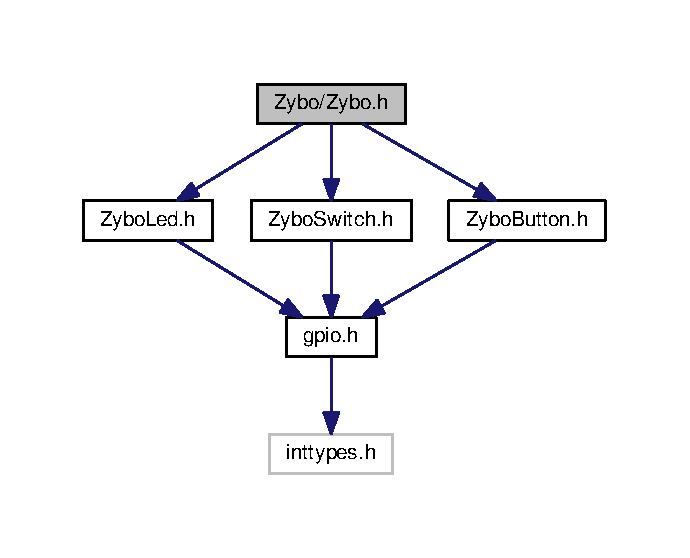
\includegraphics[width=331pt]{_zybo_8h__incl}
\end{center}
\end{figure}


\subsection{Descrizione dettagliata}
\begin{DoxyAuthor}{Autore}
Salvatore Barone \href{mailto:salvator.barone@gmail.com}{\tt salvator.\+barone@gmail.\+com}
\end{DoxyAuthor}
\begin{DoxyCopyright}{Copyright}
Copyright 2017 Salvatore Barone \href{mailto:salvator.barone@gmail.com}{\tt salvator.\+barone@gmail.\+com}
\end{DoxyCopyright}
This file is part of Zynq7000\+Driver\+Pack

Zynq7000\+Driver\+Pack is free software; you can redistribute it and/or modify it under the terms of the G\+NU General Public License as published by the Free Software Foundation; either version 3 of the License, or any later version.

Zynq7000\+Driver\+Pack is distributed in the hope that it will be useful, but W\+I\+T\+H\+O\+UT A\+NY W\+A\+R\+R\+A\+N\+TY; without even the implied warranty of M\+E\+R\+C\+H\+A\+N\+T\+A\+B\+I\+L\+I\+TY or F\+I\+T\+N\+E\+SS F\+OR A P\+A\+R\+T\+I\+C\+U\+L\+AR P\+U\+R\+P\+O\+SE. See the G\+NU General Public License for more details.

You should have received a copy of the G\+NU General Public License along with this program; if not, write to the Free Software Foundation, Inc., 51 Franklin Street, Fifth Floor, Boston, MA 02110-\/1301, U\+SA. 
\hypertarget{_zybo_button_8c}{\section{Riferimenti per il file Zybo/\+Zybo\+Button.c}
\label{_zybo_button_8c}\index{Zybo/\+Zybo\+Button.\+c@{Zybo/\+Zybo\+Button.\+c}}
}
{\ttfamily \#include \char`\"{}Zybo\+Button.\+h\char`\"{}}\\*
{\ttfamily \#include $<$assert.\+h$>$}\\*
{\ttfamily \#include $<$stdlib.\+h$>$}\\*
Grafo delle dipendenze di inclusione per Zybo\+Button.\+c\+:
\nopagebreak
\begin{figure}[H]
\begin{center}
\leavevmode
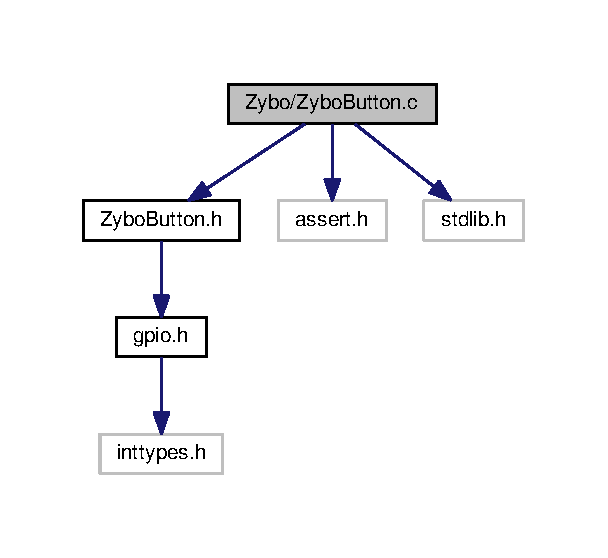
\includegraphics[width=292pt]{_zybo_button_8c__incl}
\end{center}
\end{figure}
\subsection*{Definizioni}
\begin{DoxyCompactItemize}
\item 
\#define \hyperlink{_zybo_button_8c_a5f45c877d1e8266f8a2c1d0b87746950}{timer\+\_\+wait\+\_\+ms}(ms)~usleep(ms$<$$<$10)
\end{DoxyCompactItemize}
\subsection*{Funzioni}
\begin{DoxyCompactItemize}
\item 
void \hyperlink{group___button_gaa40462223af93b0f5bdf2932400fe2a5}{Zybo\+Button\+\_\+init} (\hyperlink{struct_zybo_button__t}{Zybo\+Button\+\_\+t} $\ast$buttons, G\+P\+I\+O\+\_\+t $\ast$gpio, G\+P\+I\+O\+\_\+mask Button3\+\_\+pin, G\+P\+I\+O\+\_\+mask Button2\+\_\+pin, G\+P\+I\+O\+\_\+mask Button1\+\_\+pin, G\+P\+I\+O\+\_\+mask Button0\+\_\+pin)
\begin{DoxyCompactList}\small\item\em Inizializza un oggetto di tipo \hyperlink{struct_zybo_button__t}{Zybo\+Button\+\_\+t}. \end{DoxyCompactList}\item 
void \hyperlink{group___button_gaca30e81084e746785e395f79e9678e9a}{Zybo\+Button\+\_\+wait\+While\+Idle} (\hyperlink{struct_zybo_button__t}{Zybo\+Button\+\_\+t} $\ast$buttons)
\begin{DoxyCompactList}\small\item\em Permettere di mettere il programma in attesa attiva finche' i button restano inattivi;. \end{DoxyCompactList}\item 
void \hyperlink{group___button_ga3840edf011b5bad6302b7efc9c6326fe}{Zybo\+Button\+\_\+wait\+While\+Busy} (\hyperlink{struct_zybo_button__t}{Zybo\+Button\+\_\+t} $\ast$buttons)
\begin{DoxyCompactList}\small\item\em Permettere di mettere il programma in attesa attiva finche' i button restano attivi;. \end{DoxyCompactList}\item 
\hyperlink{group___button_ga85c290bfa232cab213e69200bf78e06a}{Zybo\+Button\+\_\+status\+\_\+t} \hyperlink{group___button_ga75407539e8ba0ad3ea142496219cd083}{Zybo\+Button\+\_\+get\+Status} (\hyperlink{struct_zybo_button__t}{Zybo\+Button\+\_\+t} $\ast$buttons, \hyperlink{group___button_ga4d26a5f6cad606de534ba034e0ba42dd}{Zybo\+Button\+\_\+mask\+\_\+t} mask)
\begin{DoxyCompactList}\small\item\em Permette la lettura dello stato dei button presenti sulla board. \end{DoxyCompactList}\end{DoxyCompactItemize}


\subsection{Documentazione delle definizioni}
\hypertarget{_zybo_button_8c_a5f45c877d1e8266f8a2c1d0b87746950}{\index{Zybo\+Button.\+c@{Zybo\+Button.\+c}!timer\+\_\+wait\+\_\+ms@{timer\+\_\+wait\+\_\+ms}}
\index{timer\+\_\+wait\+\_\+ms@{timer\+\_\+wait\+\_\+ms}!Zybo\+Button.\+c@{Zybo\+Button.\+c}}
\subsubsection[{timer\+\_\+wait\+\_\+ms}]{\setlength{\rightskip}{0pt plus 5cm}\#define timer\+\_\+wait\+\_\+ms(
\begin{DoxyParamCaption}
\item[{}]{ms}
\end{DoxyParamCaption}
)~usleep(ms$<$$<$10)}}\label{_zybo_button_8c_a5f45c877d1e8266f8a2c1d0b87746950}

\hypertarget{_zybo_button_8h}{\section{Riferimenti per il file Zybo/\+Zybo\+Button.h}
\label{_zybo_button_8h}\index{Zybo/\+Zybo\+Button.\+h@{Zybo/\+Zybo\+Button.\+h}}
}
{\ttfamily \#include \char`\"{}gpio.\+h\char`\"{}}\\*
Grafo delle dipendenze di inclusione per Zybo\+Button.\+h\+:\nopagebreak
\begin{figure}[H]
\begin{center}
\leavevmode
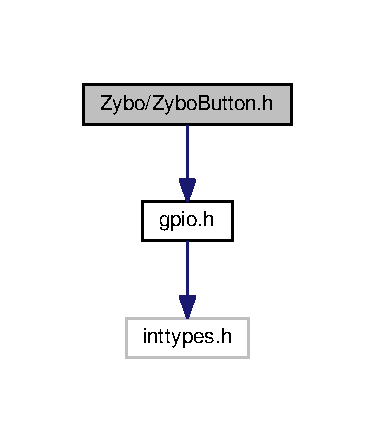
\includegraphics[width=180pt]{_zybo_button_8h__incl}
\end{center}
\end{figure}
Questo grafo mostra quali altri file includono direttamente o indirettamente questo file\+:\nopagebreak
\begin{figure}[H]
\begin{center}
\leavevmode
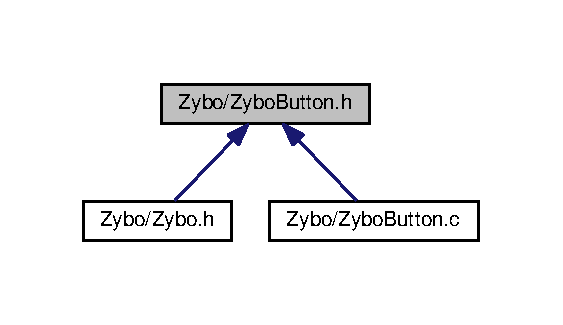
\includegraphics[width=270pt]{_zybo_button_8h__dep__incl}
\end{center}
\end{figure}
\subsection*{Strutture dati}
\begin{DoxyCompactItemize}
\item 
struct \hyperlink{struct_zybo_button__t}{Zybo\+Button\+\_\+t}
\begin{DoxyCompactList}\small\item\em Struttura opaca che astrae l'insieme dei button presenti sulla board Digilent Zybo;. \end{DoxyCompactList}\end{DoxyCompactItemize}
\subsection*{Definizioni}
\begin{DoxyCompactItemize}
\item 
\#define \hyperlink{group___button_ga5f85cbc14732f1d83faa75500b67defa}{Zybo\+Button}(i)~((uint32\+\_\+t)(1$<$$<$i))
\begin{DoxyCompactList}\small\item\em Metodo alternativo per la specifica di uno dei button presenti sulla board Digilent Zybo. \end{DoxyCompactList}\item 
\#define \hyperlink{group___button_ga8960eefa6a431f50d4fe2a2f8063da3f}{Zybo\+Button\+\_\+\+Debounce\+Wait}~50
\begin{DoxyCompactList}\small\item\em Tempo di attesa (in millisecondi) usato per prevenire il fenomeno del bouncing. Il valore di default è 50, determinato empiricamente. Puo' essere modificato a piacimento cambiando il valore alla macro seguente. \end{DoxyCompactList}\end{DoxyCompactItemize}
\subsection*{Tipi enumerati (enum)}
\begin{DoxyCompactItemize}
\item 
enum \hyperlink{group___button_ga4d26a5f6cad606de534ba034e0ba42dd}{Zybo\+Button\+\_\+mask\+\_\+t} \{ \hyperlink{group___button_gga4d26a5f6cad606de534ba034e0ba42ddaabede392be8cae14b8a070a804c754e8}{Zybo\+Button3} = 0x8, 
\hyperlink{group___button_gga4d26a5f6cad606de534ba034e0ba42dda2aa888c8f01ac8a79013e5ebc9eef609}{Zybo\+Button2} = 0x4, 
\hyperlink{group___button_gga4d26a5f6cad606de534ba034e0ba42dda29c35ef3133898c050f675a60de66dd7}{Zybo\+Button1} = 0x2, 
\hyperlink{group___button_gga4d26a5f6cad606de534ba034e0ba42dda2f821ce9661687aefb0ec4de65911570}{Zybo\+Button0} = 0x1
 \}
\begin{DoxyCompactList}\small\item\em Maschere di selezione dei Push\+Button. \end{DoxyCompactList}\item 
enum \hyperlink{group___button_ga85c290bfa232cab213e69200bf78e06a}{Zybo\+Button\+\_\+status\+\_\+t} \{ \hyperlink{group___button_gga85c290bfa232cab213e69200bf78e06aacd110f28912806bcec929721e8737399}{Zybo\+Button\+\_\+off}, 
\hyperlink{group___button_gga85c290bfa232cab213e69200bf78e06aa49bf4a6902270f28bc6a1146fbd1b1fe}{Zybo\+Button\+\_\+on}
 \}
\begin{DoxyCompactList}\small\item\em Status di attivo/inattivo dei Push\+Button. \end{DoxyCompactList}\end{DoxyCompactItemize}
\subsection*{Funzioni}
\begin{DoxyCompactItemize}
\item 
void \hyperlink{group___button_gaa40462223af93b0f5bdf2932400fe2a5}{Zybo\+Button\+\_\+init} (\hyperlink{struct_zybo_button__t}{Zybo\+Button\+\_\+t} $\ast$buttons, \hyperlink{struct_g_p_i_o__t}{G\+P\+I\+O\+\_\+t} $\ast$gpio, \hyperlink{group___g_p_i_o_ga6d5aef8a8a54ee2f602d47252ff66595}{G\+P\+I\+O\+\_\+mask} Button3\+\_\+pin, \hyperlink{group___g_p_i_o_ga6d5aef8a8a54ee2f602d47252ff66595}{G\+P\+I\+O\+\_\+mask} Button2\+\_\+pin, \hyperlink{group___g_p_i_o_ga6d5aef8a8a54ee2f602d47252ff66595}{G\+P\+I\+O\+\_\+mask} Button1\+\_\+pin, \hyperlink{group___g_p_i_o_ga6d5aef8a8a54ee2f602d47252ff66595}{G\+P\+I\+O\+\_\+mask} Button0\+\_\+pin)
\begin{DoxyCompactList}\small\item\em Inizializza un oggetto di tipo \hyperlink{struct_zybo_button__t}{Zybo\+Button\+\_\+t}. \end{DoxyCompactList}\item 
void \hyperlink{group___button_gaca30e81084e746785e395f79e9678e9a}{Zybo\+Button\+\_\+wait\+While\+Idle} (\hyperlink{struct_zybo_button__t}{Zybo\+Button\+\_\+t} $\ast$buttons)
\begin{DoxyCompactList}\small\item\em Permettere di mettere il programma in attesa attiva finche' i button restano inattivi;. \end{DoxyCompactList}\item 
void \hyperlink{group___button_ga3840edf011b5bad6302b7efc9c6326fe}{Zybo\+Button\+\_\+wait\+While\+Busy} (\hyperlink{struct_zybo_button__t}{Zybo\+Button\+\_\+t} $\ast$buttons)
\begin{DoxyCompactList}\small\item\em Permettere di mettere il programma in attesa attiva finche' i button restano attivi;. \end{DoxyCompactList}\item 
\hyperlink{group___button_ga85c290bfa232cab213e69200bf78e06a}{Zybo\+Button\+\_\+status\+\_\+t} \hyperlink{group___button_ga75407539e8ba0ad3ea142496219cd083}{Zybo\+Button\+\_\+get\+Status} (\hyperlink{struct_zybo_button__t}{Zybo\+Button\+\_\+t} $\ast$buttons, \hyperlink{group___button_ga4d26a5f6cad606de534ba034e0ba42dd}{Zybo\+Button\+\_\+mask\+\_\+t} mask)
\begin{DoxyCompactList}\small\item\em Permette la lettura dello stato dei button presenti sulla board. \end{DoxyCompactList}\end{DoxyCompactItemize}

\hypertarget{_zybo_led_8c}{\section{Riferimenti per il file Zybo/\+Zybo\+Led.c}
\label{_zybo_led_8c}\index{Zybo/\+Zybo\+Led.\+c@{Zybo/\+Zybo\+Led.\+c}}
}
{\ttfamily \#include \char`\"{}Zybo\+Led.\+h\char`\"{}}\\*
{\ttfamily \#include $<$assert.\+h$>$}\\*
{\ttfamily \#include $<$stdlib.\+h$>$}\\*
Grafo delle dipendenze di inclusione per Zybo\+Led.\+c\+:\nopagebreak
\begin{figure}[H]
\begin{center}
\leavevmode
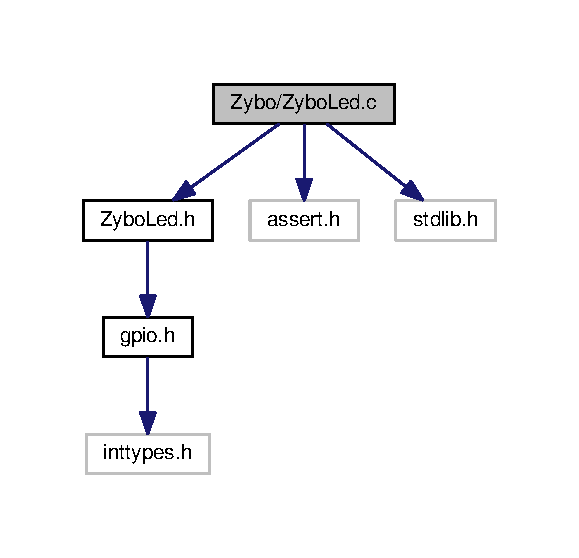
\includegraphics[width=279pt]{_zybo_led_8c__incl}
\end{center}
\end{figure}
\subsection*{Funzioni}
\begin{DoxyCompactItemize}
\item 
static int \hyperlink{_zybo_led_8c_a2a3452033228e251b3897e89a8ebcc7e}{validate\+Pair} (\hyperlink{struct_zybo_led__t}{Zybo\+Led\+\_\+t} $\ast$leds)
\item 
void \hyperlink{group___led_ga51bccd37e6ae8cd32e2c50c60a5e83cc}{Zybo\+Led\+\_\+init} (\hyperlink{struct_zybo_led__t}{Zybo\+Led\+\_\+t} $\ast$leds, \hyperlink{structmy_g_p_i_o__t}{my\+G\+P\+I\+O\+\_\+t} $\ast$gpio, \hyperlink{group__my_g_p_i_o_ga402a0d20afc0cb7c25554b8b023f4253}{my\+G\+P\+I\+O\+\_\+mask} Led3\+\_\+pin, \hyperlink{group__my_g_p_i_o_ga402a0d20afc0cb7c25554b8b023f4253}{my\+G\+P\+I\+O\+\_\+mask} Led2\+\_\+pin, \hyperlink{group__my_g_p_i_o_ga402a0d20afc0cb7c25554b8b023f4253}{my\+G\+P\+I\+O\+\_\+mask} Led1\+\_\+pin, \hyperlink{group__my_g_p_i_o_ga402a0d20afc0cb7c25554b8b023f4253}{my\+G\+P\+I\+O\+\_\+mask} Led0\+\_\+pin)
\begin{DoxyCompactList}\small\item\em Inizializza un oggetto di tipo \hyperlink{struct_zybo_led__t}{Zybo\+Led\+\_\+t}. \end{DoxyCompactList}\item 
void \hyperlink{group___led_gacf5c2b0328c4bdf2d796397fc4510c69}{Zybo\+Led\+\_\+set\+Status} (\hyperlink{struct_zybo_led__t}{Zybo\+Led\+\_\+t} $\ast$leds, \hyperlink{group___led_gad11701cccac394f7e1f90de8f85695f3}{Zybo\+Led\+\_\+mask\+\_\+t} mask, \hyperlink{group___led_ga3dcb274f22e577705c49944b8d1f4b12}{Zybo\+Led\+\_\+status\+\_\+t} status)
\begin{DoxyCompactList}\small\item\em Permette di accendere/spegnere i Led sulla board. \end{DoxyCompactList}\item 
void \hyperlink{group___led_ga20ddd78a98b4c0123c5b964aa0a59046}{Zybo\+Led\+\_\+toggle} (\hyperlink{struct_zybo_led__t}{Zybo\+Led\+\_\+t} $\ast$leds, \hyperlink{group___led_gad11701cccac394f7e1f90de8f85695f3}{Zybo\+Led\+\_\+mask\+\_\+t} mask)
\begin{DoxyCompactList}\small\item\em Permette di accendere/spegnere i Led sulla board, invertendone il valore. \end{DoxyCompactList}\end{DoxyCompactItemize}


\subsection{Descrizione dettagliata}
\begin{DoxyAuthor}{Autore}
Salvatore Barone \href{mailto:salvator.barone@gmail.com}{\tt salvator.\+barone@gmail.\+com}
\end{DoxyAuthor}
\begin{DoxyCopyright}{Copyright}
Copyright 2017 Salvatore Barone \href{mailto:salvator.barone@gmail.com}{\tt salvator.\+barone@gmail.\+com}
\end{DoxyCopyright}
This file is part of Zynq7000\+Driver\+Pack

Zynq7000\+Driver\+Pack is free software; you can redistribute it and/or modify it under the terms of the G\+N\+U General Public License as published by the Free Software Foundation; either version 3 of the License, or any later version.

Zynq7000\+Driver\+Pack is distributed in the hope that it will be useful, but W\+I\+T\+H\+O\+U\+T A\+N\+Y W\+A\+R\+R\+A\+N\+T\+Y; without even the implied warranty of M\+E\+R\+C\+H\+A\+N\+T\+A\+B\+I\+L\+I\+T\+Y or F\+I\+T\+N\+E\+S\+S F\+O\+R A P\+A\+R\+T\+I\+C\+U\+L\+A\+R P\+U\+R\+P\+O\+S\+E. See the G\+N\+U General Public License for more details.

You should have received a copy of the G\+N\+U General Public License along with this program; if not, write to the Free Software Foundation, Inc., 51 Franklin Street, Fifth Floor, Boston, M\+A 02110-\/1301, U\+S\+A. 

\subsection{Documentazione delle funzioni}
\hypertarget{_zybo_led_8c_a2a3452033228e251b3897e89a8ebcc7e}{\index{Zybo\+Led.\+c@{Zybo\+Led.\+c}!validate\+Pair@{validate\+Pair}}
\index{validate\+Pair@{validate\+Pair}!Zybo\+Led.\+c@{Zybo\+Led.\+c}}
\subsubsection[{validate\+Pair}]{\setlength{\rightskip}{0pt plus 5cm}static int validate\+Pair (
\begin{DoxyParamCaption}
\item[{{\bf Zybo\+Led\+\_\+t} $\ast$}]{leds}
\end{DoxyParamCaption}
)\hspace{0.3cm}{\ttfamily [static]}}}\label{_zybo_led_8c_a2a3452033228e251b3897e89a8ebcc7e}

\hypertarget{_zybo_led_8h}{\section{Riferimenti per il file Zybo/\+Zybo\+Led.h}
\label{_zybo_led_8h}\index{Zybo/\+Zybo\+Led.\+h@{Zybo/\+Zybo\+Led.\+h}}
}
{\ttfamily \#include \char`\"{}my\+G\+P\+I\+O.\+h\char`\"{}}\\*
Grafo delle dipendenze di inclusione per Zybo\+Led.\+h\+:\nopagebreak
\begin{figure}[H]
\begin{center}
\leavevmode
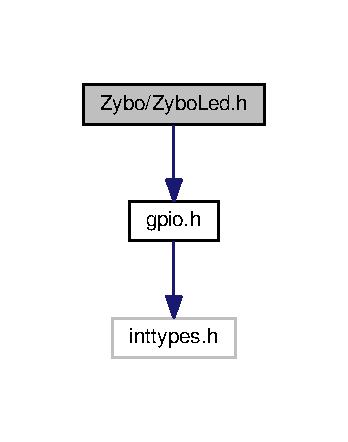
\includegraphics[width=167pt]{_zybo_led_8h__incl}
\end{center}
\end{figure}
Questo grafo mostra quali altri file includono direttamente o indirettamente questo file\+:\nopagebreak
\begin{figure}[H]
\begin{center}
\leavevmode
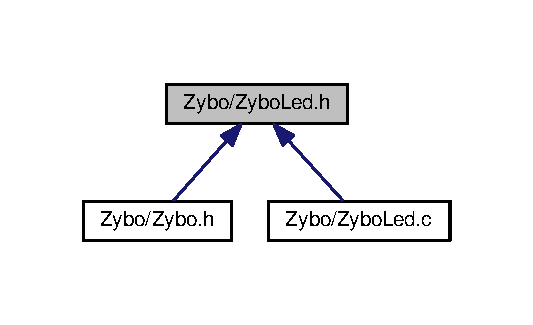
\includegraphics[width=256pt]{_zybo_led_8h__dep__incl}
\end{center}
\end{figure}
\subsection*{Strutture dati}
\begin{DoxyCompactItemize}
\item 
struct \hyperlink{struct_zybo_led__t}{Zybo\+Led\+\_\+t}
\begin{DoxyCompactList}\small\item\em Struttura opaca che astrae l'insieme dei Led presenti sulla board Digilent Zybo;. \end{DoxyCompactList}\end{DoxyCompactItemize}
\subsection*{Definizioni}
\begin{DoxyCompactItemize}
\item 
\#define \hyperlink{group___led_ga50ab39fed34dc3aaf53cdfd67d8ba25d}{Zybo\+Led}(i)~((uint32\+\_\+t)(1$<$$<$(i)))
\begin{DoxyCompactList}\small\item\em Metodo alternativo per la specifica di uno dei led presenti sulla board Digilent Zybo. \end{DoxyCompactList}\end{DoxyCompactItemize}
\subsection*{Tipi enumerati (enum)}
\begin{DoxyCompactItemize}
\item 
enum \hyperlink{group___led_gad11701cccac394f7e1f90de8f85695f3}{Zybo\+Led\+\_\+mask\+\_\+t} \{ \hyperlink{group___led_ggad11701cccac394f7e1f90de8f85695f3adc5edc2adfd899da9f149cb61364b141}{Zybo\+Led3} = 0x8\+U, 
\hyperlink{group___led_ggad11701cccac394f7e1f90de8f85695f3a4fa521f6fce7c4ba77d1d8144e71cdfc}{Zybo\+Led2} = 0x4\+U, 
\hyperlink{group___led_ggad11701cccac394f7e1f90de8f85695f3ad71c06f65dfffcf825d48f287718d9be}{Zybo\+Led1} = 0x2\+U, 
\hyperlink{group___led_ggad11701cccac394f7e1f90de8f85695f3ae1a1e8fa0bf803793ff27004884b85fe}{Zybo\+Led0} = 0x1\+U
 \}
\begin{DoxyCompactList}\small\item\em Maschere di selezione dei led. \end{DoxyCompactList}\item 
enum \hyperlink{group___led_ga3dcb274f22e577705c49944b8d1f4b12}{Zybo\+Led\+\_\+status\+\_\+t} \{ \hyperlink{group___led_gga3dcb274f22e577705c49944b8d1f4b12a9679f1c302afdb51915a2331b4ec92f3}{Zybo\+Led\+\_\+off}, 
\hyperlink{group___led_gga3dcb274f22e577705c49944b8d1f4b12aafcf0ae16a6edec807c06bb0a99f7e8b}{Zybo\+Led\+\_\+on}
 \}
\begin{DoxyCompactList}\small\item\em Status di accensione/spegnimento dei led. \end{DoxyCompactList}\end{DoxyCompactItemize}
\subsection*{Funzioni}
\begin{DoxyCompactItemize}
\item 
void \hyperlink{group___led_ga51bccd37e6ae8cd32e2c50c60a5e83cc}{Zybo\+Led\+\_\+init} (\hyperlink{struct_zybo_led__t}{Zybo\+Led\+\_\+t} $\ast$leds, \hyperlink{structmy_g_p_i_o__t}{my\+G\+P\+I\+O\+\_\+t} $\ast$gpio, \hyperlink{group__my_g_p_i_o_ga402a0d20afc0cb7c25554b8b023f4253}{my\+G\+P\+I\+O\+\_\+mask} Led3\+\_\+pin, \hyperlink{group__my_g_p_i_o_ga402a0d20afc0cb7c25554b8b023f4253}{my\+G\+P\+I\+O\+\_\+mask} Led2\+\_\+pin, \hyperlink{group__my_g_p_i_o_ga402a0d20afc0cb7c25554b8b023f4253}{my\+G\+P\+I\+O\+\_\+mask} Led1\+\_\+pin, \hyperlink{group__my_g_p_i_o_ga402a0d20afc0cb7c25554b8b023f4253}{my\+G\+P\+I\+O\+\_\+mask} Led0\+\_\+pin)
\begin{DoxyCompactList}\small\item\em Inizializza un oggetto di tipo \hyperlink{struct_zybo_led__t}{Zybo\+Led\+\_\+t}. \end{DoxyCompactList}\item 
void \hyperlink{group___led_gacf5c2b0328c4bdf2d796397fc4510c69}{Zybo\+Led\+\_\+set\+Status} (\hyperlink{struct_zybo_led__t}{Zybo\+Led\+\_\+t} $\ast$leds, \hyperlink{group___led_gad11701cccac394f7e1f90de8f85695f3}{Zybo\+Led\+\_\+mask\+\_\+t} mask, \hyperlink{group___led_ga3dcb274f22e577705c49944b8d1f4b12}{Zybo\+Led\+\_\+status\+\_\+t} status)
\begin{DoxyCompactList}\small\item\em Permette di accendere/spegnere i Led sulla board. \end{DoxyCompactList}\item 
void \hyperlink{group___led_ga20ddd78a98b4c0123c5b964aa0a59046}{Zybo\+Led\+\_\+toggle} (\hyperlink{struct_zybo_led__t}{Zybo\+Led\+\_\+t} $\ast$leds, \hyperlink{group___led_gad11701cccac394f7e1f90de8f85695f3}{Zybo\+Led\+\_\+mask\+\_\+t} mask)
\begin{DoxyCompactList}\small\item\em Permette di accendere/spegnere i Led sulla board, invertendone il valore. \end{DoxyCompactList}\end{DoxyCompactItemize}


\subsection{Descrizione dettagliata}
\begin{DoxyAuthor}{Autore}
Salvatore Barone \href{mailto:salvator.barone@gmail.com}{\tt salvator.\+barone@gmail.\+com}
\end{DoxyAuthor}
\begin{DoxyCopyright}{Copyright}
Copyright 2017 Salvatore Barone \href{mailto:salvator.barone@gmail.com}{\tt salvator.\+barone@gmail.\+com}
\end{DoxyCopyright}
This file is part of Zynq7000\+Driver\+Pack

Zynq7000\+Driver\+Pack is free software; you can redistribute it and/or modify it under the terms of the G\+N\+U General Public License as published by the Free Software Foundation; either version 3 of the License, or any later version.

Zynq7000\+Driver\+Pack is distributed in the hope that it will be useful, but W\+I\+T\+H\+O\+U\+T A\+N\+Y W\+A\+R\+R\+A\+N\+T\+Y; without even the implied warranty of M\+E\+R\+C\+H\+A\+N\+T\+A\+B\+I\+L\+I\+T\+Y or F\+I\+T\+N\+E\+S\+S F\+O\+R A P\+A\+R\+T\+I\+C\+U\+L\+A\+R P\+U\+R\+P\+O\+S\+E. See the G\+N\+U General Public License for more details.

You should have received a copy of the G\+N\+U General Public License along with this program; if not, write to the Free Software Foundation, Inc., 51 Franklin Street, Fifth Floor, Boston, M\+A 02110-\/1301, U\+S\+A. 
\hypertarget{_zybo_switch_8c}{\section{Riferimenti per il file Zybo/\+Zybo\+Switch.c}
\label{_zybo_switch_8c}\index{Zybo/\+Zybo\+Switch.\+c@{Zybo/\+Zybo\+Switch.\+c}}
}
{\ttfamily \#include \char`\"{}Zybo\+Switch.\+h\char`\"{}}\\*
{\ttfamily \#include $<$assert.\+h$>$}\\*
{\ttfamily \#include $<$stdlib.\+h$>$}\\*
Grafo delle dipendenze di inclusione per Zybo\+Switch.\+c\+:\nopagebreak
\begin{figure}[H]
\begin{center}
\leavevmode
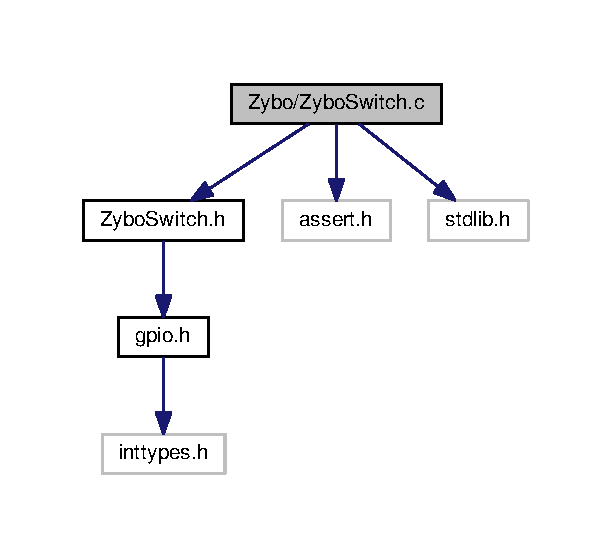
\includegraphics[width=294pt]{_zybo_switch_8c__incl}
\end{center}
\end{figure}
\subsection*{Funzioni}
\begin{DoxyCompactItemize}
\item 
void \hyperlink{group___switch_ga121018c0ccfeb05b6e8f692a5a6955d7}{Zybo\+Switch\+\_\+init} (\hyperlink{struct_zybo_switch__t}{Zybo\+Switch\+\_\+t} $\ast$switches, \hyperlink{struct_g_p_i_o__t}{G\+P\+I\+O\+\_\+t} $\ast$gpio, \hyperlink{group___g_p_i_o_ga6d5aef8a8a54ee2f602d47252ff66595}{G\+P\+I\+O\+\_\+mask} Switch3\+\_\+pin, \hyperlink{group___g_p_i_o_ga6d5aef8a8a54ee2f602d47252ff66595}{G\+P\+I\+O\+\_\+mask} Switch2\+\_\+pin, \hyperlink{group___g_p_i_o_ga6d5aef8a8a54ee2f602d47252ff66595}{G\+P\+I\+O\+\_\+mask} Switch1\+\_\+pin, \hyperlink{group___g_p_i_o_ga6d5aef8a8a54ee2f602d47252ff66595}{G\+P\+I\+O\+\_\+mask} Switch0\+\_\+pin)
\begin{DoxyCompactList}\small\item\em Inizializza un oggetto di tipo \hyperlink{struct_zybo_switch__t}{Zybo\+Switch\+\_\+t}. \end{DoxyCompactList}\item 
\hyperlink{group___switch_ga4ba6b49b2f47ebb464aefcea7e23e04a}{Zybo\+Switch\+\_\+status\+\_\+t} \hyperlink{group___switch_gafac8daf9a9a585f8f20ef2a6fa883a1f}{Zybo\+Switch\+\_\+get\+Status} (\hyperlink{struct_zybo_switch__t}{Zybo\+Switch\+\_\+t} $\ast$switches, \hyperlink{group___switch_ga2e0602a824354f25c395f938caba3703}{Zybo\+Switch\+\_\+mask\+\_\+t} mask)
\begin{DoxyCompactList}\small\item\em Permette la lettura dello stato degli switch presenti sulla board. \end{DoxyCompactList}\end{DoxyCompactItemize}

\hypertarget{_zybo_switch_8h}{\section{Riferimenti per il file Zybo/\+Zybo\+Switch.h}
\label{_zybo_switch_8h}\index{Zybo/\+Zybo\+Switch.\+h@{Zybo/\+Zybo\+Switch.\+h}}
}
{\ttfamily \#include \char`\"{}gpio.\+h\char`\"{}}\\*
Grafo delle dipendenze di inclusione per Zybo\+Switch.\+h\+:
\nopagebreak
\begin{figure}[H]
\begin{center}
\leavevmode
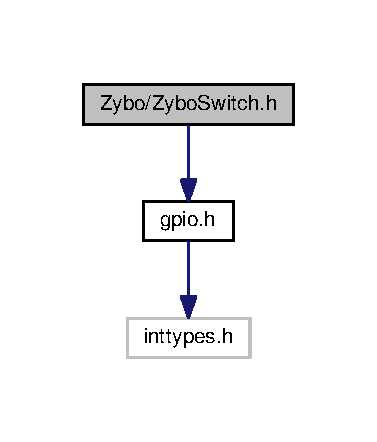
\includegraphics[width=181pt]{_zybo_switch_8h__incl}
\end{center}
\end{figure}
Questo grafo mostra quali altri file includono direttamente o indirettamente questo file\+:
\nopagebreak
\begin{figure}[H]
\begin{center}
\leavevmode
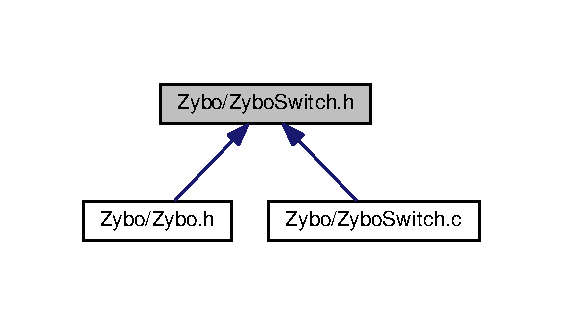
\includegraphics[width=270pt]{_zybo_switch_8h__dep__incl}
\end{center}
\end{figure}
\subsection*{Strutture dati}
\begin{DoxyCompactItemize}
\item 
struct \hyperlink{struct_zybo_switch__t}{Zybo\+Switch\+\_\+t}
\begin{DoxyCompactList}\small\item\em Struttura opaca che astrae l'insieme degli switch presenti sulla board Digilent Zybo;. \end{DoxyCompactList}\end{DoxyCompactItemize}
\subsection*{Definizioni}
\begin{DoxyCompactItemize}
\item 
\#define \hyperlink{group___switch_ga1c463f6e1e3a43f68109c176772ce5cc}{Zybo\+Switch}(i)~((uint32\+\_\+t)(1$<$$<$i))
\begin{DoxyCompactList}\small\item\em Metodo alternativo per la specifica di uno degli switch presenti sulla board Digilent Zybo. \end{DoxyCompactList}\end{DoxyCompactItemize}
\subsection*{Tipi enumerati (enum)}
\begin{DoxyCompactItemize}
\item 
enum \hyperlink{group___switch_ga2e0602a824354f25c395f938caba3703}{Zybo\+Switch\+\_\+mask\+\_\+t} \{ \hyperlink{group___switch_gga2e0602a824354f25c395f938caba3703a73ccea5ad8c919fe962e9a67a3733ee3}{Zybo\+Switch3} = 0x8\+U, 
\hyperlink{group___switch_gga2e0602a824354f25c395f938caba3703aac2f5ebb28eb3bd93fcdf8019b6a3e9e}{Zybo\+Switch2} = 0x4\+U, 
\hyperlink{group___switch_gga2e0602a824354f25c395f938caba3703a694a25c87b1ec597d2a6032bf5d34b0f}{Zybo\+Switch1} = 0x2\+U, 
\hyperlink{group___switch_gga2e0602a824354f25c395f938caba3703a84350e8b6e7a7e2cabf22fc7a1a5c651}{Zybo\+Switch0} = 0x1\+U
 \}
\begin{DoxyCompactList}\small\item\em Maschere di selezione degli switch. \end{DoxyCompactList}\item 
enum \hyperlink{group___switch_ga4ba6b49b2f47ebb464aefcea7e23e04a}{Zybo\+Switch\+\_\+status\+\_\+t} \{ \hyperlink{group___switch_gga4ba6b49b2f47ebb464aefcea7e23e04aa1d686faf83e8606e68eec0b7e525a755}{Zybo\+Switch\+\_\+off}, 
\hyperlink{group___switch_gga4ba6b49b2f47ebb464aefcea7e23e04aafba009508b8822de867af69034e3e4f8}{Zybo\+Switch\+\_\+on}
 \}
\begin{DoxyCompactList}\small\item\em Status di attivo/inattivo degli switch. \end{DoxyCompactList}\end{DoxyCompactItemize}
\subsection*{Funzioni}
\begin{DoxyCompactItemize}
\item 
void \hyperlink{group___switch_ga121018c0ccfeb05b6e8f692a5a6955d7}{Zybo\+Switch\+\_\+init} (\hyperlink{struct_zybo_switch__t}{Zybo\+Switch\+\_\+t} $\ast$switches, G\+P\+I\+O\+\_\+t $\ast$gpio, G\+P\+I\+O\+\_\+mask Switch3\+\_\+pin, G\+P\+I\+O\+\_\+mask Switch2\+\_\+pin, G\+P\+I\+O\+\_\+mask Switch1\+\_\+pin, G\+P\+I\+O\+\_\+mask Switch0\+\_\+pin)
\begin{DoxyCompactList}\small\item\em Inizializza un oggetto di tipo \hyperlink{struct_zybo_switch__t}{Zybo\+Switch\+\_\+t}. \end{DoxyCompactList}\item 
\hyperlink{group___switch_ga4ba6b49b2f47ebb464aefcea7e23e04a}{Zybo\+Switch\+\_\+status\+\_\+t} \hyperlink{group___switch_gafac8daf9a9a585f8f20ef2a6fa883a1f}{Zybo\+Switch\+\_\+get\+Status} (\hyperlink{struct_zybo_switch__t}{Zybo\+Switch\+\_\+t} $\ast$switches, \hyperlink{group___switch_ga2e0602a824354f25c395f938caba3703}{Zybo\+Switch\+\_\+mask\+\_\+t} mask)
\begin{DoxyCompactList}\small\item\em Permette la lettura dello stato degli switch presenti sulla board. \end{DoxyCompactList}\end{DoxyCompactItemize}

%--- End generated contents ---

% Index
\newpage
\phantomsection
\addcontentsline{toc}{chapter}{Indice}
\printindex

\end{document}
